% !TEX program = xelatex
% =============================================================
%  家庭数学辅导手册 · 二年级上册（北师大版）
%  主体文件 —— 用 xelatex 编译两次，或直接运行 build.ps1
% =============================================================
\documentclass[UTF8,zihao=-4,a4paper,twoside,fontset=windows]{ctexart}

% =============================================================
%  preamble.tex  --  家庭数学辅导手册（北师大版 二年级上册）公共样式
%  编译：xelatex（TeX Live 2025 / Windows 字体）
% =============================================================

% ---------- 页面 ----------
\usepackage{geometry}
\geometry{a4paper,top=2.3cm,bottom=2.2cm,left=2.0cm,right=2.0cm,
          headheight=15pt,headsep=0.45cm,footskip=1.0cm}

% ---------- 表格与列表 ----------
\usepackage{array}
\usepackage{booktabs}
\usepackage{longtable}
\usepackage{tabularx}
\usepackage{multirow}
\usepackage{makecell}
\usepackage{enumitem}
\setlist[itemize]{leftmargin=1.6em,topsep=2pt,itemsep=1.5pt,parsep=0pt}
\setlist[enumerate]{leftmargin=1.9em,topsep=2pt,itemsep=2pt,parsep=0pt}

% ---------- 数学与符号 ----------
\usepackage{amsmath}
\usepackage{amssymb}

% ---------- 颜色 ----------
\usepackage{xcolor}
\definecolor{mainc}{HTML}{0F6E68}     % 主色：墨绿
\definecolor{matc}{HTML}{B45309}      % 材料：赭
\definecolor{sayc}{HTML}{1D4ED8}      % 话术：蓝
\definecolor{pitc}{HTML}{B91C1C}      % 易错：红
\definecolor{passc}{HTML}{15803D}     % 验收：绿
\definecolor{playc}{HTML}{6D28D9}     % 游戏：紫
\definecolor{tipc}{HTML}{334155}      % 提示：石墨

% ---------- 框 ----------
\usepackage[most]{tcolorbox}
\tcbuselibrary{breakable,skins}

% ---------- 绘图 ----------
\usepackage{tikz}
\usetikzlibrary{calc,positioning,patterns,shapes.geometric,arrows.meta,decorations.pathreplacing}

% 辅导课主框
\newtcolorbox{lesson}[2]{enhanced,breakable,
  colback=white,colframe=mainc,coltitle=white,
  boxrule=1pt,arc=2mm,left=7pt,right=7pt,top=11pt,bottom=6pt,
  before skip=16pt, after skip=10pt,
  title={\heiti 任务 #1\hspace{0.6em}\normalfont\small 约 #2 分钟},
  attach boxed title to top left={xshift=4mm,yshift=-2.4mm},
  boxed title style={colback=mainc,arc=1.2mm,boxrule=0pt,
                     left=5pt,right=5pt,top=1pt,bottom=1pt},
  fonttitle=\bfseries}

% 材料/道具
\newtcolorbox{materials}{enhanced,breakable,
  colback=matc!4,colframe=matc!75,
  boxrule=0.7pt,arc=1.5mm,left=7pt,right=7pt,top=5pt,bottom=5pt,
  title={\heiti 先备货},coltitle=white,colbacktitle=matc!80,
  fonttitle=\bfseries,breakable}

% 家长话术
\newtcolorbox{saybox}{enhanced,breakable,
  colback=sayc!4,colframe=sayc!65,
  boxrule=0.7pt,arc=1.5mm,left=7pt,right=7pt,top=5pt,bottom=5pt,
  title={\heiti 照这样问小豆角},coltitle=white,colbacktitle=sayc!70,
  fonttitle=\bfseries,fontupper=\kaishu}

% 易错
\newtcolorbox{pitbox}{enhanced,breakable,
  colback=pitc!4,colframe=pitc!65,
  boxrule=0.7pt,arc=1.5mm,left=7pt,right=7pt,top=5pt,bottom=5pt,
  title={\heiti 翻车预警},coltitle=white,colbacktitle=pitc!70,
  fonttitle=\bfseries,breakable}

% 验收
\newtcolorbox{passbox}{enhanced,breakable,
  colback=passc!5,colframe=passc!70,
  boxrule=0.7pt,arc=1.5mm,left=7pt,right=7pt,top=5pt,bottom=5pt,
  title={\heiti 过关条件},coltitle=white,colbacktitle=passc!75,
  fonttitle=\bfseries,breakable}

% 游戏
\newtcolorbox{playbox}[1]{enhanced,breakable,
  colback=playc!5,colframe=playc!65,
  boxrule=0.7pt,arc=1.5mm,left=7pt,right=7pt,top=5pt,bottom=5pt,
  title={\heiti 玩法：#1},coltitle=white,colbacktitle=playc!70,
  fonttitle=\bfseries,breakable}

% 提示
\newtcolorbox{tipbox}{enhanced,breakable,
  colback=tipc!4,colframe=tipc!55,boxrule=0.7pt,arc=1.5mm,
  left=7pt,right=7pt,top=4pt,bottom=4pt,fontupper=\small}

% 答案
\newtcolorbox{ansbox}{enhanced,breakable,
  colback=black!3,colframe=black!25,boxrule=0.5pt,arc=1mm,
  left=6pt,right=6pt,top=3pt,bottom=3pt,fontupper=\small\kaishu}

% ---------- 趣味三件套 ----------
% 豆角爸爸翻车现场
\newtcolorbox{blunder}{enhanced,breakable,
  colback=black!3,colframe=black!50,
  boxrule=0.7pt,arc=1.5mm,left=8pt,right=8pt,top=5pt,bottom=5pt,
  title={\heiti 豆角爸爸翻车现场},coltitle=white,colbacktitle=black!58,
  fonttitle=\bfseries,fontupper=\kaishu}

% 赌一把
\newtcolorbox{gamble}[1]{enhanced,breakable,
  colback=matc!7,colframe=matc,
  boxrule=1.1pt,arc=1.5mm,left=8pt,right=8pt,top=5pt,bottom=5pt,
  title={\heiti #1},coltitle=white,colbacktitle=matc,
  fonttitle=\bfseries}

% 彩蛋任务
\newtcolorbox{bonus}{enhanced,breakable,
  colback=playc!5,colframe=playc!75,
  frame style={dash pattern=on 5pt off 3pt},
  boxrule=1.1pt,arc=1.5mm,left=8pt,right=8pt,top=5pt,bottom=5pt,
  title={\heiti 彩蛋任务（不算分，纯粹好玩）},coltitle=white,colbacktitle=playc!75,
  fonttitle=\bfseries}

% 单人旁白（开玩笑用）
\newtcolorbox{aside}{enhanced,breakable,
  colback=white,colframe=black!20,boxrule=0.5pt,
  left=8pt,right=8pt,top=3pt,bottom=3pt,fontupper=\kaishu\small}

% 单元信息条
\newtcolorbox{unitinfo}{enhanced,breakable,
  colback=mainc!5,colframe=mainc!60,boxrule=0.7pt,arc=1.5mm,
  left=7pt,right=7pt,top=5pt,bottom=5pt}

% ---------- 中文字符分类修正 ----------
% 圈码（①②③）、几何图形（▲■●）、杂项符号（★）在 Unicode 里属“东亚模糊宽度”，
% xeCJK 默认会把它们交给西文字体，导致渲染成空白。这里强制归入 CJK。
\xeCJKDeclareCharClass{CJK}{"2460 -> "24FF, "25A0 -> "25FF, "2600 -> "26FF, "3007}

% ---------- 页眉页脚 ----------
\usepackage{fancyhdr}
\usepackage{lastpage}
\newcommand{\currentchapter}{}
\pagestyle{fancy}
\fancyhf{}
\fancyhead[L]{\small\color{tipc}北师大版·数学二年级上册·家庭辅导手册}
\fancyhead[R]{\small\color{tipc}\currentchapter}
\fancyfoot[C]{\small\color{tipc}\thepage\,/\,\pageref{LastPage}}
\renewcommand{\headrulewidth}{0.4pt}
\renewcommand{\headrule}{\hbox to\headwidth{\color{mainc!50}\leaders\hrule height \headrulewidth\hfill}}
\fancypagestyle{plain}{\fancyhf{}\fancyfoot[C]{\small\color{tipc}\thepage\,/\,\pageref{LastPage}}\renewcommand{\headrulewidth}{0pt}}

% ---------- 章节样式 ----------
\ctexset{
  section/numbering=false,
  subsection/numbering=false,
  subsubsection/numbering=false,
  section/format={\raggedright\Large\heiti\color{mainc}},
  section/beforeskip={6pt},
  section/afterskip={10pt},
  section/tocline={\large\heiti\selectfont#2},
  subsection/format={\raggedright\large\heiti\color{mainc!90}},
  subsection/beforeskip={14pt},
  subsection/afterskip={6pt},
  subsubsection/format={\raggedright\normalsize\heiti\color{tipc}},
  subsubsection/beforeskip={8pt},
  subsubsection/afterskip={4pt},
}

% 章标题宏：清页 + 设页眉
\newcommand{\Chapter}[1]{%
  \clearpage
  \renewcommand{\currentchapter}{#1}%
  \section{#1}%
  \noindent{\color{mainc!35}\rule{\linewidth}{0.8pt}}\par\vspace{2pt}}

% ---------- 常用小工具 ----------
% 填空下划线
\newcommand{\blank}[1][2.6em]{\underline{\hspace{#1}}}
% 书写横线
\newcommand{\wls}[1][1]{%
  \par\noindent
  \foreach \x in {1,...,#1}{\makebox[\linewidth][l]{\color{gray!55}\dotfill}\par\vspace{3.4mm}}}
% 复选框
\newcommand{\cb}{\tikz[baseline=-0.55ex]{\draw[tipc!70,line width=0.6pt](0,0)rectangle(0.4,0.4);}\hspace{0.35em}}
% 星星
\newcommand{\starx}{\textcolor{matc}{$\bigstar$}}
% 竖式块（1 列运算符 + 3 列数字，定宽右对齐 → 每一位自动对齐）
\newcolumntype{O}{>{\raggedleft\arraybackslash}p{0.85em}}
\newcolumntype{D}{>{\raggedleft\arraybackslash}p{0.68em}}
\newenvironment{shushi}{%
  \par\smallskip\noindent\renewcommand{\arraystretch}{1.08}%
  \begin{tabular}{@{}O D D D@{}}
}{%
  \end{tabular}\par\smallskip}
% 同上，但可放进 tabular 单元格里并排使用
\newenvironment{shushicell}{%
  \renewcommand{\arraystretch}{1.08}%
  \begin{tabular}{@{}O D D D@{}}
}{%
  \end{tabular}}
% 高亮
\newcommand{\key}[1]{\textcolor{mainc}{\heiti #1}}
% 页码引用
\newcommand{\seep}[1]{{\small\color{tipc}（教材 P#1）}}

% ---------- 超链接（放最后） ----------
\usepackage[bookmarksnumbered,bookmarksopen,hidelinks]{hyperref}
\usepackage{bookmark}

\renewcommand{\contentsname}{目\hspace{1em}录}


\begin{document}

% ---------- 封面 ----------
% =============================================================
%  封面
% =============================================================
\thispagestyle{empty}

\vspace*{1.6cm}

\begin{center}

{\color{mainc!25}\rule{\linewidth}{2.2pt}}\\[2pt]
{\color{mainc!25}\rule{\linewidth}{0.6pt}}

\vspace{2.4cm}

{\heiti\fontsize{38}{48}\selectfont\color{mainc} 豆角家庭辅导执行手册}

\vspace{0.5cm}

{\heiti\fontsize{26}{34}\selectfont\color{mainc!85} 数学}

\vspace{0.9cm}

{\kaishu\fontsize{17}{26}\selectfont\color{tipc} 二年级上册（北师大版）}

\vfill

\begin{tikzpicture}
  \node[draw=mainc!45,line width=0.8pt,rounded corners=2pt,
        fill=white,inner sep=14pt,text width=9.6cm,align=left]
  {%
   \kaishu\fontsize{12}{24}\selectfont
   \textbf{作\hspace{2em}者}：豆角爸爸 \\[2pt]
   \textbf{编\hspace{2em}辑}：豆角爸爸 \\[2pt]
   \textbf{校\hspace{2em}对}：豆角爸爸 \\[2pt]
   \textbf{编辑时间}：2026 年 7 月  \\[2pt]
   \textbf{定稿时间}：2026 年 10 月
  };
\end{tikzpicture}

\vfill

{\color{mainc!25}\rule{\linewidth}{0.6pt}}\\[9pt]
{\small\color{tipc} 豆角爸爸\quad https://www.bd7iwd.com}\\[9pt]
{\color{mainc!25}\rule{\linewidth}{2.2pt}}

\vspace{0.5cm}

{\small\color{tipc} 依据北京师范大学出版社《数学》二年级上册（2025 年 7 月第 1 版）编写}

\end{center}

\clearpage


% ---------- 目录 ----------
\clearpage
\pagestyle{plain}
\tableofcontents
\pagestyle{fancy}
\MakeHeaders

% ---------- 家长使用说明 ----------
% =============================================================
%  开局说明
% =============================================================
\Chapter{开局说明：这套东西怎么玩}

\begin{unitinfo}
先说清楚：\textbf{这不是练习册。}里面一道“口算天天练”都没有。\\
它是一份\textbf{陪小豆角闯关的说明书}——豆角爸爸照着念、照着做，
二十分钟一到，收工，谁也不许加练。
\end{unitinfo}

\subsection{出场人物}

\begin{center}
\begin{tabularx}{\linewidth}{@{}p{2.6cm}X@{}}
\toprule
\textbf{小豆角} & 二年级，本书唯一的服务对象。强项是记性好，弱项是缺乏逻辑思维且在数学上长期得不到正向反馈，导致
对数学约错越怕，越怕越错，对数学产生恐惧。 \\
\textbf{豆角爸爸} & 本书作者、编辑、校对，以及\textbf{头号翻车选手}。
心算经常错，量东西经常量错，剪窗花像剪怪兽。\\
\textbf{棒子弟} & 那包小棒。一百根，捆起来的时候会“变身”——
十根一捆，就变成了“一个十”。 \\
\textbf{啪嗒哥} & 五档计数器。往上推珠子会“啪嗒”一声，
\textbf{借位的时候它最忙}，连着啪嗒两下。 \\
\textbf{剪刀姐} & 专门负责对称。她对“折痕有没有对齐”这件事非常挑剔。 \\
\bottomrule
\end{tabularx}
\end{center}

\subsection{闯关地图}

一共八关，加一个隐藏关，最后是终局。\textbf{每一关都对着课本的一个单元}，
所以学校讲到哪儿，豆角爸爸就跳到哪一关。

\begin{center}
\begin{tikzpicture}[font=\scriptsize,
  box/.style={draw=mainc,rounded corners=1.2mm,fill=mainc!6,inner sep=3pt,
              minimum width=3.45cm,minimum height=0.95cm,align=center,text width=3.4cm}]
  \node[box] (n1) at (0,0) {\textbf{1}\ 一串小棒走天下};
  \node[box] (n2) at (3.95,0) {\textbf{2}\ 尺子、绳子和一双大手};
  \node[box] (n3) at (7.9,0) {\textbf{3}\ 把加法压扁};
  \node[box] (n4) at (11.85,0) {\textbf{4}\ 编顺口溜的人};
  \node[box] (n5) at (11.85,-1.35) {\textbf{5}\ 分东西，不许打架};
  \node[box] (n6) at (7.9,-1.35) {\textbf{6}\ 剪一刀，动一下};
  \node[box] (n7) at (3.95,-1.35) {\textbf{7}\ 八九七十二的来历};
  \node[box] (n8) at (0,-1.35) {\textbf{8}\ 算账的本事};
  \node[box] (n9) at (0,-2.7) {\textbf{隐藏}\ 画地图，花真钱};
  \node[box] (n10) at (3.95,-2.7) {\textbf{终局}\ 考前三十天};
  \foreach \a/\b in {n1/n2,n2/n3,n3/n4,n5/n6,n6/n7,n7/n8}{
    \draw[-{Stealth},mainc,thick] (\a) -- (\b);}
  \draw[-{Stealth},mainc,thick] (n4) -- (n5);
  \draw[-{Stealth},mainc,thick] (n8) -- (n9);
  \draw[-{Stealth},mainc,thick] (n9) -- (n10);
\end{tikzpicture}
\end{center}

\noindent{\small\color{tipc}
对照：第 1 关＝课本第一单元（100 以内加与减）· 第 2 关＝测量 · 第 3 关＝数一数与乘法 ·
第 4 关＝乘法口诀（一）· 第 5 关＝分一分与除法 · 第 6 关＝图形的运动 ·
第 7 关＝乘法口诀（二）· 第 8 关＝乘除法的应用 · 隐藏关＝两次综合实践 · 终局＝总复习}

\subsection{每一关里有什么}

每关的结构都一样。重点是下面这三件“玩的东西”，
它们不是点缀，\textbf{是让小豆角愿意坐下来的唯一理由}。

\begin{blunder}
\textbf{豆角爸爸的翻车现场}。每关开头，爸爸先自曝一个真实糗事：
量错床单、剪出怪兽、算错找零。
\textbf{作用}：让小豆角知道“错”不是丢人的事，爸爸错得比小豆角多。
\end{blunder}

\begin{gamble}{课前协商：这一页最要紧}
每关开头都有一个\textbf{课前协商}框：\textbf{今天比什么}由这本书来定，
\textbf{赢了拿什么、输了认什么}留空——\textbf{上课前两分钟谈好，当场手写填上去}。\\[4pt]
根据豆角现阶段最想要的东西设计正向激励。\\[5pt]
\textbf{三条铁律}（很重要，别破坏）：
\begin{enumerate}[label=\arabic*、]
  \item \textbf{豆角爸爸一定要真的输一次。}全程赢的爸爸，小豆角不会想再跟爸爸玩了。
  \item \textbf{赌注要小、要当场兑现。}小到不用心疼，近到当天能兑现；
        别赌“考好了给小豆角买xx”。
  \item \textbf{先让小豆角开口提。}她自己提的赌注，她才认账；爸爸只负责把它压小一点。
\end{enumerate}
\end{gamble}

\begin{bonus}
每关还有一个\textbf{跟分数完全没关系}的野任务：电梯挑战、身高排行榜、
把口诀唱成 rap、藏宝图、当一天家庭采购员。\\
\textbf{作用}：把数学塞进小豆角本来就爱干的事里。做了不加分，不做也不骂。
\end{bonus}

\subsection{二十分钟怎么切}

说实话，真正“讲”的时间只有两分钟。剩下全是小豆角在动手。
这不是偷懒，这是小豆角唯一能吸收的方式。

\begin{center}
\begin{tabularx}{\linewidth}{@{}p{1.4cm}p{2.3cm}X@{}}
\toprule
\textbf{时间} & \textbf{干什么} & \textbf{爸爸干什么} \\
\midrule
3 分钟 & 抽卡口算 & 抽十张，小豆角报答案。爸爸只记对错，\textbf{当场不纠}。\\
2 分钟 & 小豆角自己读题 & 爸爸只说一句“把数字圈出来”。\textbf{爸爸不念题}，一念小豆角就不看题了。\\
8 分钟 & \textbf{上手摆} & 全场最重要的八分钟。爸爸发东西，小豆角摆，爸爸不可以说话。\\
5 分钟 & 落到纸上 & 小豆角写算式、竖式或口诀。\textbf{一个字爸爸都不代笔}。\\
2 分钟 & 收尾 & 三句：今天学了啥？哪步最容易翻车？明天还来吗？\\
\bottomrule
\end{tabularx}
\end{center}

\subsection{三种开法，挑一种}

\begin{center}
\begin{tabularx}{\linewidth}{@{}p{2.6cm}p{2.4cm}X@{}}
\toprule
\textbf{开法} & \textbf{节奏} & \textbf{适合什么情况} \\
\midrule
\textbf{跟着学校走} & 一周 2 次 & 周二、周四晚上各一次，
学校讲完哪个单元，爸爸就翻到那一关。一学期 41 次，刚好放到期末。\\
\textbf{假期先扫一遍} & 一周 5 次 & 寒暑假集中过，开学前把整册摸完。
开学后上课就等于复习，小豆角会很轻松。\\
\textbf{哪儿着火灭哪儿} & 一周 3 次 & 竖式老错、口诀背不下来，
就只打那一关。先做关末的抽查，找出病根，再往回补。\\
\bottomrule
\end{tabularx}
\end{center}

\noindent 不管选哪种，这三条别动：
\textbf{① 一次不超过 25 分钟；② 一次只推进一个点；③ 结束前让小豆角自己复述一遍。}

\subsection{爸爸的约定}

\begin{enumerate}
  \item \textbf{二十分钟到点就停。}没做完也停。宁可明天再来，别今天把小豆角磨烦。
  \item \textbf{不抢答。}小豆角停五秒爸爸才开口。五秒是小豆角把话组织出来的正常时间。
  \item \textbf{新的东西，第一次必须上手。}小棒也好纸片也好手指也好，
        先摆出来，摆完才许写算式。
  \item \textbf{小豆角做错了，爸爸先问“小豆角是怎么想的”。}不先说“错了”。
        让小豆角把错路走完，爸爸才知道断在哪。
  \item \textbf{一次只教一个点。}今天搞“进位”，就别顺嘴讲“退位”。
        讲了等于两个都没讲。
  \item \textbf{“这么简单都不会”这句话，一次都不说。}换成“这步确实容易忘，再看一遍”。
  \item \textbf{爸爸也不许掏手机算。}宁可一起重新摆一遍。
  \item \textbf{允许小豆角比爸爸慢。}小豆角摆十五根小棒花四十秒，正常。
  \item \textbf{每次留一个好印象。}收尾必须指着一件小豆角做对的事说清楚：
        “今天小豆角自己想到要捆起来，这个很关键。”
  \item \textbf{课前谈好的当场兑现。}输了就认，不许拖到明天。
\end{enumerate}

\noindent{\small\color{tipc}正文里出现\,\waterdrop\,的地方，是给爸爸的暗号：
“这里可以让一步，放点水。”小豆角不用懂。}

\subsection{爸爸自己踩过的六个坑}

\begin{pitbox}
\begin{enumerate}[label=\arabic*、]
  \item \textbf{把规则直接说出口。}“个位满十向十位进一”，爸爸一说，小豆角抄下来，
        看着像会了。换一组数又不会了。\\
        \textbf{改法}：让小豆角自己把十根捆成一捆，然后问小豆角“这一捆从哪来的”。
        让小豆角自己说出“十根换一捆”——这句话是小豆角说的，才管用。
  \item \textbf{拿口诀顶替理解。}小豆角能背“六七四十二”，但不知道怎么画出来。
        题目一改成“画图表示”，交白卷。\\
        \textbf{改法}：每句新口诀，先在点子图或百数表上圈出那块地方，圈完再背。
  \item \textbf{管小豆角掰手指。}爸爸一开始也管，说“多大了还掰手指”。
        结果小豆角改成在桌子底下偷偷数，还多了一层紧张。\\
        \textbf{改法}：见下一节，掰手指有明确的时间表，到点自然撤。
  \item \textbf{用题量顶思考。}一口气一百道口算，小豆角刷完还是不会。\\
        \textbf{改法}：一种类型做透五道，比五十道管用。
  \item \textbf{边做边纠错。}小豆角写一步爸爸说一次“不对”，最后小豆角干脆停手等爸爸报答案。\\
        \textbf{改法}：整道题做完，再一起回头看。
  \item \textbf{盯着分数。}二年级上册真正的目标是“能说清为什么”。
        说不清却做对，是运气；说得清但算错，是进步。
\end{enumerate}
\end{pitbox}

\subsection{掰手指这事儿，说清楚}

不管，但要有退出时间表。

\begin{center}
\begin{tabularx}{\linewidth}{@{}p{3.6cm}X@{}}
\toprule
\textbf{什么时候} & \textbf{允许小豆角用手吗} \\
\midrule
第 1 关 & 随便掰。\textbf{别催}。这阶段目标是“懂”，不是“快”。\\
第 2--4 关 & 20 以内还能掰；两位数的进位加、退位减
\textbf{必须用小棒或竖式}。手指不够用，正好自然过渡。\\
第 5--8 关 & 口诀必须脱手，直接报数；除法可以心里想口诀。\\
终局 & 100 以内加减，允许小豆角在心里想竖式，不再动手。\\
\bottomrule
\end{tabularx}
\end{center}

\noindent \textbf{怎么判断该不该管}，看两件事就够：

\begin{itemize}
  \item \textbf{又慢又准} $\to$ 正常，别管，小豆角在认真算。
  \item \textbf{又快又错} $\to$ 小豆角在猜，必须退回“摆”。
  \item \textbf{又慢又错} $\to$ 某一步根本没懂，退回上一关重来。
\end{itemize}

\subsection{错题本：一次只写一句话}

不要抄整道题。抄题小豆角会烦，抄完也不会看。

\begin{itemize}
  \item 这样写：\ “48+25，个位 8+5=13，爸爸把进的 1 忘了加到十位。”
  \item 不要这样写：\ “粗心”“算错了”“不认真”——一条都别写，写了等于没写。
\end{itemize}

\noindent 每周日花五分钟，让小豆角读一遍自己写的错因，然后口头重做那三道题。做对就划掉。

\textbf{同一个错因出现三次，停课，回去补那一关。}
这是整本书最重要的一条判断依据，比任何分数都准。

\subsection{战利品：星星，和赢爸爸一次}

二年级小豆角对分数没感觉，对贴纸和“赢爸爸一次”很有感觉。

\begin{itemize}
  \item 一次课顺顺当当上完（不哭、不跑、没超时）$\to$ \starx\ 一颗。
  \item 一次抽查全对 $\to$ \starx\ 一颗。
  \item \textbf{小豆角自己发现并改了一个错} $\to$ \starx\starx\ 两颗。
        \textbf{这条最重要}，爸爸在刻意鼓励小豆角自查，这个比做对更有价值。
  \item 攒够 20 颗，换一次小豆角自己点单的东西。
\end{itemize}

\noindent \textbf{底线}：不用“考一百分”、“考第一”当条件。

\subsection{每次开打前，三分钟准备}

\begin{enumerate}
  \item \cb 课本翻到这一关标的页码了吗？
  \item \cb “先备货”框里的东西都拿到了吗？缺一样就先去找，别用“凑合”代替。
  \item \cb 桌子清空了吗？只留课本、笔、材料。玩具和平板收走。
  \item \cb 计时器设 20 分钟，放在小豆角看得见的地方。
  \item \cb 爸爸自己把“照这样问小豆角”看过一遍了吗？\textbf{提前看，别现场编。}
\end{enumerate}

\noindent 五条都打钩再开始。\textbf{准备不足就改天，别硬上}——
硬上浪费时间。


% ---------- 道具材料清单 ----------
% =============================================================
%  要买的东西
% =============================================================
\Chapter{开工前：要买什么、翻什么、印什么}
\phantomsection\label{chap:supplies}

\begin{unitinfo}
二年级上册凡是“摆一摆、量一量、剪一剪、买一买”的地方，都得有东西上手。
没东西，小豆角就只能看爸爸拿笔在纸上画——那跟看视频没区别，学不进去。\\
\textbf{一次买齐，整学期不用再跑文具店。}清单不长，看着像玩具，其实是这学期最要紧的一套家伙。
\end{unitinfo}

\subsection{为什么非要买小棒}

一包小棒，看着像玩具，其实是这学期最核心的一件教具。

因为\textbf{十进制这件事，只能用“捆”来解释}。爸爸说“满十进一”，
小豆角的脑子里没有画面；爸爸把 13 根散的让小豆角自己捆成一捆，
小豆角手上就有了一个动作：\textbf{10 根变成 1 捆}。
这个动作重复十几次，小豆角才真的知道“十位”是什么东西。

同样的道理：
\begin{itemize}
  \item \textbf{计数器}——解释“100 减 48 借不到怎么办”，比小棒更直观（珠子一挪就看得见）。
  \item \textbf{直尺}——不摸尺子，“1 厘米”永远是个词。
  \item \textbf{硬币纸币}——不算钱，“1 元 = 10 角”就是背书。
\end{itemize}

\subsection{要买的（16 样）}

\begin{center}
\small
\begin{tabularx}{\linewidth}{@{}p{0.5cm}p{3.2cm}p{4.8cm}p{1.0cm}X@{}}
\toprule
\textbf{序} & \textbf{买什么} & \textbf{怎么挑} & \textbf{几份} & \textbf{用在哪} \\
\midrule
1 & 小棒 & 木质或塑料计数棒，一包 100 根。\textbf{重点：要能捆}，别买成一整块塑料板 &
      2 包 & 全书主力，一、三、四、五、七、八单元 \\
2 & 计数器 & 五档（个十百千万），每档 10 颗珠 & 1 个 & 第一单元进位退位、第二单元读数 \\
3 & 透明直尺 15\,cm & 刻度清楚，0 刻度在最边上 & 2 把 & 第二单元，两把能接起来量长的 \\
4 & 透明直尺 30\,cm & 同上 & 1 把 & 第二单元量课桌、书本 \\
5 & 软尺 & 1.5 米裁缝尺 & 1 条 & 第二单元量黑板、身高 \\
6 & 正方形手工纸 & 15\,cm$\times$15\,cm，100 张。\textbf{用量很大} & 1 包 & 第六单元剪对称 \\
7 & A4 彩色卡纸 & 20 张，多色 & 1 包 & 做陀螺、竹蜻蜓、价格牌 \\
8 & 儿童剪刀 & 圆头 & 1 把 & 第六单元 \\
9 & 固体胶 & 1 支 & 1 支 & 贴记录、做手工 \\
10 & 塑料吸管 & 普通饮料吸管，50 支 & 1 包 & 第六单元竹蜻蜓 \\
11 & 竹签／牙签 & 一头尖 & 1 盒 & 第六单元陀螺中轴 \\
12 & 图钉 & 1 盒 & 1 盒 & 第六单元风车、陀螺 \\
13 & 骰子 & 六面，1--6 点 & 2 颗 & 第五单元火星探险、口算游戏 \\
14 & 棋子 & 跳棋那种小圆片 & 1 副 & 第五单元棋盘 \\
15 & 贴纸 & 100 张装 & 1 包 & 全书星星奖励 \\
16 & 打印复印 & A4 约 30 页，其中 4 页用 160\,g 卡纸 & 1 次 & 附录全部 \\
\bottomrule
\end{tabularx}
\end{center}

\subsection{想再加点（可选）}

\begin{center}
\small
\begin{tabularx}{\linewidth}{@{}p{0.5cm}p{3.2cm}p{9.0cm}p{1.0cm}@{}}
\toprule
\textbf{序} & \textbf{买什么} & \textbf{为什么值} & \textbf{几份} \\
\midrule
17 & 磁性小白板 45$\times$60 & 讲竖式、画图能反复擦，比纸省事太多。
      不想买就\textbf{把 A4 白纸塞进透明文件袋}，用白板笔写，效果差不多 & 1 块 \\
18 & 收纳盒 & 3 个带盖的，分“计数／手工／纸品”，贴标签 & 3 个 \\
19 & 扑克牌 & 抽牌比大小、凑十、口诀对练，一学期都用得上 & 1 副 \\
\bottomrule
\end{tabularx}
\end{center}

\subsection{家里翻出来的}

\begin{center}
\small
\begin{tabularx}{\linewidth}{@{}p{3.4cm}Xp{3.0cm}@{}}
\toprule
\textbf{翻什么} & \textbf{拿来干嘛} & \textbf{哪个单元} \\
\midrule
1 米长的绳子／鞋带 & 剪成正好 1 米，去比家里哪些东西比 1 米长 & 第二单元 \\
豆子／玻璃珠／弹弓子弹 & 当计数物，比小棒好摆成堆 & 一、三、五单元 \\
纸杯 6 个 & 当盘子、袋子、笼子，做平均分 & 第五单元 \\
小饼干／糖果一包 & 分东西的真实版，\textbf{分完能吃} & 第五单元 \\
快递纸箱 & 拆开做华容道底板、陀螺纸板 & 第六单元 \\
旧杂志／报纸 & 练剪直线曲线，剪坏了不心疼 & 第六单元 \\
皮筋 10 根 & 把小棒捆成十根一捆，进位全靠它 & 第一单元 \\
手机 & 指南针（认方向）、计时、拍下小豆角的作品 & 全单元 \\
卷尺 & 量身高、量家具 & 第二单元 \\
透明文件袋 & 塞白纸当白板用 & 全单元 \\
\bottomrule
\end{tabularx}
\end{center}

\subsection{要印的（本书附录，约 30 页）}

\begin{center}
\small
\begin{tabularx}{\linewidth}{@{}p{1.5cm}p{5.0cm}p{1.2cm}X@{}}
\toprule
\textbf{在哪} & \textbf{印什么} & \textbf{几页} & \textbf{怎么印} \\
\midrule
附录 A & 口算卡（加减／乘法／除法，剪成小卡） & 8 页 & \textbf{160\,g 卡纸}，单面，剪开 \\
附录 B & 口诀表（完整＋填空）、百数表、数位表、方格纸 & 6 页 & 普通纸；口诀表和百数表多印两份 \\
附录 C & 模拟人民币 & 2 页 & \textbf{160\,g 卡纸}，剪开 \\
附录 D & 打卡表、错题表、星星表、速查卡 & 3 页 & 普通纸，速查卡贴冰箱 \\
第五单元内 & 火星探险棋盘 & 1 页 & 普通纸或卡纸 \\
第六单元内 & 华容道棋盘 & 1 页 & \textbf{卡纸}，剪成小块 \\
\bottomrule
\end{tabularx}
\end{center}

\begin{tipbox}
\textbf{打印一定要选“实际大小／100\%”}，千万别勾“适应页面”。
缩过的手工纸和人民币尺寸就不准了——第五单元买东西会算错钱。
\end{tipbox}

\subsection{每个单元额外要备的（前一天晚上花两分钟）}

\begin{center}
\small
\begin{tabularx}{\linewidth}{@{}p{2.2cm}X@{}}
\toprule
\textbf{单元} & \textbf{这一天额外要拿出来的} \\
\midrule

第一单元 & 小棒＋皮筋（捆十用）、计数器、骰子、方格竖式纸（附录 B） \\
第二单元 & 15\,cm 和 30\,cm 直尺、软尺、1 米绳子、
\textbf{一把“坏尺子”}（拿旧尺把 0 那头用胶带贴住，让 0 看不见） \\
第三单元 & 小棒、玻璃珠、弹弓子弹、点子图（附录 B） \\
第四单元 & 小棒、百数表、口诀卡（附录 A 的乘法卡先只用 1--5 部分） \\
第五单元 & 小棒 30 根、纸杯 6 个、一包小饼干、骰子和棋子、棋盘（本章末页） \\
第六单元 & 手工纸、卡纸、剪刀、吸管、竹签、图钉、快递纸箱 \\
第七单元 & 百数表、口诀填空表、\textbf{小豆角自己的十根手指}（9 的口诀要用） \\
第八单元 & 小棒、附录 A／B 的练习纸 \\
综合实践 & 手机指南针、A3 纸、模拟人民币、家里小物件 \\
\bottomrule
\end{tabularx}
\end{center}

\subsection{装盒，五分钟搞定}

\begin{center}
\small
\begin{tabularx}{\linewidth}{@{}p{2.4cm}p{1.0cm}X@{}}
\toprule
\textbf{盒子} & \textbf{贴的标签} & \textbf{装这些} \\
\midrule
盒 1 & 计数 & 小棒两包、皮筋、豆子、骰子、棋子、扑克牌 \\
盒 2 & 手工 & 剪刀、固体胶、手工纸、卡纸、吸管、竹签、图钉、1 米绳子 \\
盒 3 & 纸品 & 口算卡、口诀表、百数表、数位表、人民币、记录表、方格纸 \\
\bottomrule
\end{tabularx}
\end{center}

\noindent 盒 3 里再拿文件袋分一下（卡一袋、表一袋、钱一袋）。
上课前三十秒能拿全，才不会因为“找东西”把二十分钟耗掉。

\subsection{直接抄走，下单去}

\begin{tipbox}
小棒 ×2 包\quad 计数器（五档）×1\quad 透明直尺 15\,cm ×2\quad 透明直尺 30\,cm ×1\\
软尺 1.5\,m ×1\quad 正方形手工纸 15\,cm ×1 包\quad A4 彩色卡纸 ×1 包\quad 儿童剪刀 ×1\\
固体胶 ×1\quad 塑料吸管 ×1 包\quad 竹签 ×1 盒\quad 图钉 ×1 盒\\
骰子 ×2\quad 跳棋棋子 ×1 副\quad 奖励贴纸 ×1 包\\
（可选）磁性白板 ×1\quad 收纳盒 ×3\quad 扑克牌 ×1
\end{tipbox}

\noindent \textbf{优先级}：小棒、计数器、直尺、手工纸、剪刀——这五样\textbf{第一周就得到位}，
因为第一、二单元立刻要用。剩下的边用边补，不着急。


% ---------- 各单元 ----------
% =============================================================
%  第一单元  100 以内数加与减（二）
% =============================================================
\Chapter{第一关\quad 一串小棒走天下}
\noindent{\small\kaishu\color{tipc}（课本第一单元：100 以内加与减（二），P2--P17）}

\begin{blunder}
开学第一周，超市结账 48 块，爸爸给了 100，收银员找给 52。
爸爸心里“咦”了一下——怎么才找这么点？回家一算，是爸爸自己心算错了。
更尴尬的是妈妈在旁边补了一句：“一百减四十八，不就是五十二吗。”
\end{blunder}

\begin{gamble}{课前协商：五道“100 减两位数”}
\begin{itemize}
  \item 两人轮流出题：爸爸出五道给小豆角算，小豆角也出五道考爸爸。
  \item \textbf{小豆角当裁判}：爸爸做题时，小豆角负责挑错，抓到一处记一颗星。\waterdrop
  \item 三局两胜，打完当场兑现。
\end{itemize}
\negolines
\end{gamble}

\begin{bonus}
\begin{itemize}
  \item \textbf{电梯挑战}：进电梯让小豆角闭上眼，猜“从 1 楼到 12 楼经过几层”。
        到了睁眼看楼层数字。猜对一次记一颗星。
  \item \textbf{存钱罐对账}：每周数一次零花钱，算“这周比上周多了多少”。
        多出来的钱小豆角可以自己决定怎么花——这比十道应用题管用。
  \item \textbf{找零游戏}：超市结账前让小豆角先估个总数，结完对一对。
        估差在 5 块以内，这周小豆角挑一次零食。
\end{itemize}
\end{bonus}

\begin{unitinfo}
\textbf{课本 P2--P17}（外加“数学好玩·猜数游戏”P18--P19）\quad
\textbf{6 次课，每次 20 分钟} \\[4pt]
\textbf{这一关到底在干嘛}：就是把“10 根捆成 1 捆”和“拆开 1 捆当 10 根”
这两个动作，反复做到手上。\\
\textbf{为什么它最要紧}：后面乘、除、口诀，全都踩在这两个动作上。
这两个动作要是只“背下来”，到三年级学多位数、四年级学小数，会整片塌掉。
\textbf{宁可慢，也必须亲手捆、亲手拆。}
\end{unitinfo}

\subsection{开局先聊个事：这些题生活里长什么样}

爸爸今天带小豆角去超市，东西 48 块，爸爸给 100，收银员找爸爸多少？——这就是 $100-48$。

电梯在 1 楼，小豆角去 12 楼的同学家玩，中间经过几层？
——这就是“差几层”。

小豆角跳绳跳了 48 个，隔壁小朋友比小豆角多跳 25 个，人家跳多少？
——这就是“比谁多”。

课本把这些都编成了小故事（摘苹果、收玉米、跳绳），
本质是同一件事：\textbf{小豆角要是能看着东西数出来，就能算出来。}

\subsection{任务 1：把“满十进一”捆出来}

\begin{lesson}{1}{20}
\textbf{今天要拿下的}：让小豆角自己把 10 根散的小棒捆成一捆，
并且说出“这一捆是从散的那堆里来的”。

\begin{materials}
小棒 60 根、皮筋 10 根、一张白纸、一支笔。
\end{materials}

\begin{enumerate}
  \item \textbf{摆}：桌上摆 35 根——3 捆（每捆 10 根）＋ 5 根散的。
        让小豆角数一遍，说清楚“3 个十和 5 个一”。
  \item \textbf{加}：旁边再放 8 根散的。问：“现在散的一共有几根？”
        （$5+8=13$ 根）
  \item \textbf{等小豆角捆}：把皮筋递过去，只说一句：“散的有点多了，小豆角想想办法。”
        \textbf{全程不要给提示，不说话就好了}\\
        小豆角要是想不到，就提示一句：“10 根散的一捆，是什么？”
        \textbf{不要直接说“捆起来”。}
  \item \textbf{数}：捆好以后数——4 捆 ＋ 3 根散 $=43$。
  \item \textbf{写}：让小豆角自己在纸上写 $35+8=43$。
  \item \textbf{问那句关键的话}：“本来是 3 捆，怎么变成 4 捆了？”\\
        小豆角答“散的凑够 10 根，捆了一捆”——\textbf{好，这就是“满十进一”}。
        让小豆角自己说出这句话，别替小豆角说。
  \item \textbf{换题再走一遍}：$26+19$。19 得先自己捆成 1 捆＋9 根，
        然后 2 捆＋1 捆，6 根＋9 根 $=15$ 根，再捆一捆 →
        4 捆＋5 根 $=45$。
\end{enumerate}

\begin{saybox}
“这一捆是从哪里来的？”\\
“3 捆怎么变成 4 捆的？”\\
“散的满 10 根了，小豆角打算怎么办？”\\
“小豆角刚才做的这个动作，不用小棒的话，怎么记下来？”
\end{saybox}

\begin{pitbox}
\textbf{最常见的卡点}：小豆角算出“13 根散的”，然后就把 13 根散着摆在那儿，
直接数出“3 捆 + 13 根”$=43$——\textbf{答案对，但“捆”这个动作没做}。\\
\textbf{怎么办}：别纠答案（答案没错），追一句：“13 根散的，能不能变成 1 捆几根？”
让小豆角把那一捆补上。\textbf{这一课全部的价值，就在这个动作里。}
\end{pitbox}

\begin{passbox}
\begin{itemize}
  \item “摆 $\to$ 加 $\to$ 捆 $\to$ 数”四步小豆角自己走完，爸爸一根手指都不动。
  \item 小豆角能用自己的话讲清“为什么十位多了一”。
  \item 换成 $38+9$ 或 $17+25$，小豆角照样能走一遍。
\end{itemize}
\end{passbox}
\end{lesson}

\subsection{任务 2：竖式那三条规矩，和“当医生”}

\begin{lesson}{2}{20}
\textbf{今天要拿下的}：把昨天手上捆的动作，翻译成竖式上的三个规矩。

\begin{materials}
方格竖式纸（附录 B）、笔。有条件用白板，能擦了重写。
\end{materials}

\begin{enumerate}
  \item \textbf{先用手再做一遍} $38+9$，三十秒，确认动作还记得。
  \item \textbf{搬到纸上}：拿方格竖式纸，一位一格。
        \begin{center}
        \begin{tabular}{@{}c@{\hspace{1.6cm}}c@{}}
          \begin{shushicell}
            & 3 & 8\\
          + &   & 9\\ \midrule
            & 4 & 7
          \end{shushicell}
          &
          \begin{shushicell}
            & 2 & 6\\
          + & 1 & 9\\ \midrule
            & 4 & 5
          \end{shushicell}
        \end{tabular}
        \end{center}
        \textbf{边写边问}：“个位 8+9=17，格子只有一个，17 放哪？”
        （写 7，把 1 记在十位上面，用小字写。）\\
        “那个小小的 1，是 1 个一还是 1 个十？”——1 个十，所以它站十位。
  \item \textbf{连做四道}：$38+9$、$27+24$、$35+15$、$9+38$。
        每道都要求\textbf{先把进位小 1 写出来}，再算十位。
  \item \textbf{让小豆角当医生}：下面三个病人，找病因、改正。
        \begin{center}
        \begin{tabular}{@{}c@{\hspace{1.1cm}}c@{\hspace{1.1cm}}c@{}}
          \begin{shushicell}
            & 4 & 7\\
          + &   & 6\\ \midrule
            & 4 & 3
          \end{shushicell}
          &
          \begin{shushicell}
            & 3 & 6\\
          + & 2 & 9\\ \midrule
            & 5 & 5
          \end{shushicell}
          &
          \begin{shushicell}
            & 5 & 2\\
          + & 1 & 7\\ \midrule
            & 6 & 9
          \end{shushicell}
        \end{tabular}
        \end{center}
        答案：第一题 53（个位 13 只写了 3，把进的 1 丢了）；
        第二题 65（十位 3+2 忘了加进的 1）；第三题 69——\textbf{这个是对的，故意放个假病人}。
  \item \textbf{收三句话}（让小豆角自己说，爸爸写在纸上贴起来）：
        ① 个位对个位，十位对十位；② 个位满十，在十位上面写个小 1；
        ③ 十位相加时，别忘那个 1。
\end{enumerate}

\begin{saybox}
“小豆角把进的 1 放哪了？为什么放十位，不放个位？”\\
“这道题小豆角是医生，小豆角说它得了什么病？”（比“小豆角又算错了”印象更深）\\
“十位要是忘了加 1，得数会差多少？”（差 10，让小豆角自己发现）
\end{saybox}

\begin{passbox}
\begin{itemize}
  \item 5 道进位加全对，而且\textbf{每道都有进位小 1 的痕迹}。
  \item 前两个“病人”的病因小豆角自己找出来了。
\end{itemize}
\end{passbox}
\end{lesson}

\subsection{任务 3：把“退一当十”拆出来}

\begin{lesson}{3}{20}
\textbf{今天要拿下的}：小豆角会亲手拆开一捆，并说出“十位要少 1”。

\begin{materials}
小棒、皮筋、笔。
\end{materials}

\begin{enumerate}
  \item \textbf{摆} 52：5 捆＋2 根。要拿走 7 根。
  \item \textbf{先卡住小豆角}：让小豆角拿 7 根。散的只有 2 根，\textbf{拿不出来}。
        停在这儿，问：“怎么办？”
  \item \textbf{拆}：把 1 捆拆开，变 10 根散的 → 现在散的 12 根，捆的剩 4 捆。
        拿走 7 根，散剩 5 根。结果 4 捆＋5 根 $=45$。
  \item \textbf{搬到纸上}：
        \begin{center}
        \begin{shushicell}
          & 5 & 2\\
        - & 3 & 7\\ \midrule
          & 1 & 5
        \end{shushicell}
        \end{center}
        “个位 2 减 7 不够，从十位借 1 当 10，$12-7=5$；
        十位 5 已经借走 1，只剩 4，$4-3=1$。”
  \item \textbf{教一个招：退位点}。借过位的十位，在上面点一个小点。
        \textbf{看到点就先减 1}——这是防“借了忘还”的唯一办法。
        让小豆角以后每道退位题都点。
  \item \textbf{连做四道}：$52-37$、$53-26$、$32-3$、$43-14$。
  \item \textbf{当医生}：
        \begin{center}
        \begin{tabular}{@{}c@{\hspace{1.6cm}}c@{}}
          \begin{shushicell}
            & 5 & 2\\
          - &   & 8\\ \midrule
            & 5 & 4
          \end{shushicell}
          &
          \begin{shushicell}
            & 4 & 3\\
          - & 1 & 4\\ \midrule
            & 3 & 1
          \end{shushicell}
        \end{tabular}
        \end{center}
        答案：第一题 44（把 $8-2$ 倒着减了）；第二题 29（十位忘了已经借走 1）。
\end{enumerate}

\begin{saybox}
“小豆角借来的那一捆，是几个十？那十位是不是要少 1？”\\
“个位不够减，能不能拿大的减小的？”（不能——这条小豆角最想干）\\
“小豆角十位上那个点，什么时候点的？为什么点它？”
\end{saybox}

\begin{pitbox}
\textbf{三个高频错误，盯着看：}
\begin{enumerate}[label=\arabic*、]
  \item \textbf{倒着减}：$52-8$ 算成 54。\textbf{一句话}：“不够减就先借，不许倒着减。”
  \item \textbf{借了不还}：$43-14$ 算成 39。\textbf{一句话}：“点上点的那一位，先减 1 再算。”
  \item \textbf{借来的当成 1}：以为借来的是 1 而不是 10。
        \textbf{一句话}：回小棒，“小豆角拆开那一捆，是 1 根还是 10 根？”
\end{enumerate}
\end{pitbox}

\begin{passbox}
\begin{itemize}
  \item 用小棒独立做出 $52-37$，包括“拆捆”那一下。
  \item 5 道退位竖式全对，每题都有退位点。
  \item 小豆角能讲清“倒着减”为什么不对。
\end{itemize}
\end{passbox}
\end{lesson}

\subsection{任务 4：100 减两位数（难度较大·重点关注）}

\begin{lesson}{4}{25}
\textbf{今天要拿下的}：十位是 0 借不到的时候，知道“连着借两次”。

\begin{materials}
计数器（这一课\textbf{必须用}，比小棒直观得多）。
\end{materials}

\begin{enumerate}
  \item \textbf{拨} 100：只在百位拨 1 颗珠。
  \item \textbf{卡住小豆角}：要减 48。个位 0 颗，减不了 8；十位也 0 颗，借不到。
        停住，问：“怎么办？”
  \item \textbf{借两次}（让小豆角自己动手挪珠子）：
        \begin{itemize}
          \item 第一步：从百位借 1 颗放十位 → 十位变成 10 颗（$=10$ 个十）。
          \item 第二步：从十位借 1 颗放个位 → 个位 10 颗，十位剩 9 颗。
        \end{itemize}
        现在：百位 0、十位 9、个位 10。
  \item \textbf{减}：个位 $10-8=2$；十位 $9-4=5$ → 52。
  \item \textbf{写竖式}：
        \begin{center}
        \begin{shushicell}
          & 1 & 0 & 0\\
        - &   & 4 & 8\\ \midrule
          &   & 5 & 2
        \end{shushicell}
        \end{center}
        让小豆角自己：百位 1 上打点、十位 0 改成 9、个位 0 改成 10。
        \textbf{三个记号都要画出来}，画全了才算过。
  \item \textbf{连做}：$100-39$、$100-24$、$70-27$、$80-55$。
        （$70-27$ 只借一次：十位 7 借 1 给个位，个位变 10，十位剩 6，$6-2=4$ → 43。）
  \item \textbf{找一个技巧}：不会算的时候，\textbf{先估一个数}。
        $100-48$ 大概是多少？50 上下。算出来 52——就在 50 附近，\textbf{这说明小豆角没算错方向}。
        养成“先估后算”的习惯，比多做题管用。
\end{enumerate}

\begin{saybox}
“十位是 0，借不到，小豆角想向谁借？”\\
“从百位借来的 1，到了十位变成几了？”（10 个十）\\
“十位有 10 了，个位还是 0，怎么办？”（再从十位借 1）\\
“小豆角估一下，$100-48$ 大概多少？”（先估再算）
\end{saybox}

\begin{pitbox}
\textbf{两种典型错法}：
\begin{enumerate}[label=\arabic*、]
  \item 算出 62 或 68——十位当成 10 了，借了没还。\\
\textbf{解法}：让小豆角数计数器上十位到底剩几颗（9 颗），眼见为实。
  \item 直接放弃，说“不会”。\\
\textbf{解法}：一定先上计数器。纸上只是记录，动手在前面。
\end{enumerate}
\textbf{这一课别赶。}25 分钟只弄明白 $100-48$ 一道，也值。
\end{pitbox}

\begin{passbox}
\begin{itemize}
  \item 计数器上独立做出 $100-48$，并说出“借了两次”。
  \item 竖式上三个记号齐全（百位点、十位 0 改 9、个位 0 改 10）。
  \item $100-39$、$70-27$ 独立做对。
\end{itemize}
\end{passbox}
\end{lesson}

\subsection{任务 5：先画图，再列式}

\begin{lesson}{5}{20}
\textbf{今天要拿下的}：遇到“比谁多／少”，\textbf{第一反应是画一条线}，不是猜加减。

\begin{materials}
纸、笔、尺子。
\end{materials}

\begin{enumerate}
  \item \textbf{课本 P10 跳绳}：小红跳了 48 次；小亮比小红少跳 9 次；
        小东比小红多跳 25 次。问小亮、小东各跳多少。
  \item \textbf{让小豆角圈信息}：三个数字，加“多”“少”两个字，全圈出来。
  \item \textbf{画线段}（慢一点，这一步是重点）：
        \begin{center}
        \begin{tikzpicture}[x=0.14cm,y=0.95cm,font=\small]
          \draw[mainc,thick] (0,2) -- (48,2);
          \node[left] at (0,2) {小红};
          \node[above] at (24,2) {48 次};
          \draw[pitc,thick] (0,1) -- (39,1);
          \node[left] at (0,1) {小亮};
          \node[above] at (19.5,1) {比小红少 9，所以短一点};
          \draw[sayc,thick] (0,0) -- (73,0);
          \node[left] at (0,0) {小东};
          \node[above] at (60,0) {比小红多 25，所以长一点};
          \draw[dashed,gray] (48,2) -- (48,0.15);
        \end{tikzpicture}
        \end{center}
  \item \textbf{从图上读数}：小亮 $=48-9=39$（次）；小东 $=48+25=73$（次）。
  \item \textbf{反过来问一次}：小红想跳到 100 次，还要跳多少？$100-48=52$（次）。
  \item \textbf{换个场景再来一遍}（课本 P12 图书馆三层）：
        第一层 23 本，第二层比第一层多 18 本，第三层比第一层少 9 本。
        画三条线 $\to 23+18=41$、$23-9=14$。
  \item \textbf{让小豆角总结一句话}：“‘比谁多’就在谁身上加一段；‘比谁少’就减一段。
        \textbf{所以第一步是找出‘谁’是标准。}”
\end{enumerate}

\begin{saybox}
“‘比小红少’，小豆角是拿谁当标准？”\\
“小豆角能用手指在图上指出‘多出来的 25 次’是哪一段吗？”\\
“如果不画图，小豆角能保证不把加法写成减法吗？”（让小豆角自己承认画图有用）
\end{saybox}

\begin{pitbox}
\textbf{最容易翻车的地方}：小豆角看到“少 9”就减、看到“多 25”就加，形式上对了。
可换成“小亮跳了 39 次，比小红少 9 次，小红跳多少？”小豆角立刻翻车——
因为\textbf{标准换了人}。\\
\textbf{解法}：每道题先问一句“\textbf{谁是标准}”，把标准那个人画在最上面。
位置对了，加减就不会错。
\end{pitbox}

\begin{passbox}
\begin{itemize}
  \item 三条线段小豆角自己画出来（长短、标注、对齐都对）。
  \item 小豆角能看着自己的图讲“为什么这里要加、那里要减”。
  \item 反向题（知道差和一个量，求另一个）也能做。
\end{itemize}
\end{passbox}
\end{lesson}

\subsection{任务 6：闯关 + 猜数游戏}

\begin{lesson}{6}{20}
\textbf{今天要拿下的}：前五课验一遍；顺便学一个“聪明地问”的办法。

\begin{materials}
百数表（附录 B）、纸、笔。
\end{materials}

\begin{enumerate}
  \item \textbf{先做 5 分钟快检}（见本章末），错的记下来。
  \item \textbf{猜数游戏}（课本 P18--P19）：
        \begin{playbox}{猜数（只能答“对”或“不对”）}
        ① 爸爸心里想一个 1--100 的数，小豆角来猜。小豆角问，爸爸只能说“对”或“不对”。\\
        ② 数一数小豆角问了几次猜中。\\
        ③ 再来一次，第二轮爸爸示范一句：“比 50 大吗？”然后每次都问“比中间大吗”，
        让小豆角看着范围一次砍一半：$100\to50\to25\to12\to6\to3\to1$，最多 7 次。\\
        ④ 第三轮换小豆角当“想数的人”，让小豆角体会“一半一半地排除”为什么快。
        \end{playbox}
  \item \textbf{收一句话}：“每次问‘比中间大吗’，一下就去掉一半可能，
        所以 7 次一定猜得到。”——\textbf{不用讲“二分法”这个词}，二年级只要体会。
  \item \textbf{收尾}：错的题抄进错题本（只写错因一句话），贴今天的星星。
\end{enumerate}

\begin{passbox}
\begin{itemize}
  \item 快检 10 题至少对 8 题，错的能说出错在哪一步。
  \item 猜数能在 7 次以内猜中 1--100 的任意数。
\end{itemize}
\end{passbox}
\end{lesson}

\subsection{翻车现场（对着看）}

\begin{center}
\small
\begin{tabularx}{\linewidth}{@{}p{3.6cm}p{4.0cm}X@{}}
\toprule
\textbf{小豆角写出来的样子} & \textbf{其实是想错了什么} & \textbf{爸爸回一句什么} \\
\midrule
$28+35=513$ & 不知道进位是加到\textbf{十位}上，把 1 挤在个位后面 &
“进的 1 是 1 个\textbf{十}，要住十位。” \\
\addlinespace[2pt]
$52-8=54$ & 个位不够减，倒着减了 & “不够减先借，不许倒着减。” \\
\addlinespace[2pt]
$43-14=39$ & 十位忘了已经借走 1 & “点上点的那位，先减 1。” \\
\addlinespace[2pt]
$100-48$ 空着 & 十位是 0，借不到就卡死 & 先上计数器，把“借”做出来。 \\
\addlinespace[2pt]
个位十位上下错开 & 没有格子管着，靠眼睛估 & 整章只用方格竖式纸。 \\
\addlinespace[2pt]
“比……多”做成减法 & 语言和运算没接上 & 一律先画线段，标出谁是标准。 \\
\addlinespace[2pt]
算式对，答语不写 & 没有“写完”的习惯 & 最后一行必须写“答：……”。 \\
\bottomrule
\end{tabularx}
\end{center}

\subsection{抽查：随机开枪（10 题）}

\begin{enumerate}[label=\arabic*.,itemsep=4pt]
  \item $35+8=$ \blank \qquad 2. $47+9=$ \blank \qquad 3. $26+19=$ \blank
  \item $52-7=$ \blank \qquad 5. $52-37=$ \blank \qquad 6. $100-48=$ \blank
  \item $70-27=$ \blank \qquad 8. $38+9=$ \blank \qquad 9. $60-41=$ \blank
  \item $48+25=$ \blank
\end{enumerate}

\begin{ansbox}
1. 43\quad 2. 56\quad 3. 45\quad 4. 45\quad 5. 15\quad
6. 52\quad 7. 43\quad 8. 47\quad 9. 19\quad 10. 73\\
\textbf{不到 7 题对}：回任务 2、任务 3再来一遍，别急着进第二单元。
\end{ansbox}

\subsection{平时生活里怎么练（不占上课时间）}

\begin{itemize}
  \item \textbf{超市算钱}：让小豆角算“两样一共多少钱”，钱数压在 100 以内。
        再给小豆角 100 块，让小豆角算该找多少——$100-$ 两位数的真身就在这儿。
  \item \textbf{电梯}：从 1 楼到 12 楼经过几层？再下到 3 楼，往下走几层？
  \item \textbf{扑克牌凑 100}：抽两张（A 当 1，JQK 去掉），看能不能凑成整十；
        熟了以后抽三张，先凑十再加。
  \item \textbf{存钱罐}：每周数一次零花钱，让小豆角算“这周比上周多了多少”。
  \item \textbf{每天 3 分钟口算卡}：抽 10 张，只报答案不写。连续五天全对，加一颗星。
\end{itemize}

% =============================================================
%  第二单元  测量（一）
% =============================================================
\Chapter{第二关\quad 尺子、绳子和一双大手}
\noindent{\small\kaishu\color{tipc}（课本第二单元：测量（一），P20--P29）}

\begin{blunder}
去年网上买床单，豆角爸爸把“床宽”记成了“床长”，买回来短了 20 厘米。
铺上去像条围裙，四边都露着床垫。小豆角说：“豆角爸爸，这床单是不是缩水了？”
豆角爸爸没敢说是自己量错的。
\end{blunder}

\begin{gamble}{赌一把：估长度，谁准谁赢}
\begin{itemize}
  \item 随便指家里一样东西（沙发、电视、门），两个人\textbf{各写一个估计数}，不许说出口。
  \item 一起量。\textbf{谁差得少谁赢}。输的人请对方一瓶小可乐，
        \textbf{但自己一口都不能喝}。连输三天换人。
  \item 进阶：不许用尺子，只能用“爸爸的一拃”去量。这时候小豆角会发现——
        大人的一拃和小朋友的一拃，根本不是一回事。
\end{itemize}
\end{gamble}

\begin{bonus}
\begin{itemize}
  \item \textbf{身高比赛}：在门框上画线，两个人都量，做一张榜贴墙上。
        每月更新一次，让小豆角自己读数、自己记日期。\textbf{小豆角会天天去看自己长高没有。}
  \item \textbf{买鞋量脚}：让小豆角自己把脚画在纸上，量最长的那根指头到脚跟，
        记下多少厘米，对照鞋码表看对不对。
  \item \textbf{不用尺子量床}：只许用小豆角的“一拃”去量小豆角的床，报“几拃”。
        然后豆角爸爸用手量一遍，再比一比——为什么数不一样？（这一关就通了）
\end{itemize}
\end{bonus}

\begin{unitinfo}
\textbf{课本 P20--P29}\quad \textbf{5 次课，每次 20 分钟}\quad
\textbf{建议第 5--7 周} \\[4pt]
\textbf{这一关到底在干嘛}：先让小豆角吃一次“量出来不算数”的亏，
再教小豆角把尺子用对。\\
\textbf{逻辑是这么走的}：\ 大家各量各的 $\to$ 结果对不上 $\to$ 所以要有个统一的“一小段”
$\to$ 这一小段叫 1 厘米 $\to$ 10 个 10 厘米拼起来叫 1 米。\\
\textbf{小豆角最容易栽的地方}：不是读数，是\textbf{没有单位感}。
能读对尺子，却把铅笔填成“17 米”。
\end{unitinfo}

\subsection{开局先聊个事：这些事生活里天天遇到}

给小豆角买鞋，得量脚长多少厘米；网上买床单，得看床多宽；
带小豆角做核酸，脚下一米线——都是一样的东西。

至于“17 米长的铅笔”这种笑话，其实大人也常犯：
有人问豆角爸爸客厅多大，豆角爸爸说“二十来平”，问豆角爸爸多远，豆角爸爸说“走过去五分钟”。
\textbf{单位感}这件事，靠的是身体记住，不是靠背。

所以这一章分两步：\textbf{先让小豆角量乱一次，再教小豆角量准。}

\subsection{任务 1：故意让小豆角量乱一次}

\begin{lesson}{1}{20}
\textbf{今天要拿下的}：小豆角自己得出“必须用一样长的东西量，别人才听得懂”。

\begin{materials}
一张桌子（或书桌）、铅笔、筷子。\textbf{今天不给小豆角尺子。}
\end{materials}

\begin{enumerate}
  \item \textbf{给任务}：量一量这张桌子有多长。\textbf{不许用尺子。}
  \item \textbf{第一轮用手}：用“拃”（张开大拇指到中指）量，边量边数。
        记下来：“桌子有 \blank 拃长”。
  \item \textbf{第二轮用铅笔}：再量。记：“\blank 支铅笔长”。
  \item \textbf{第三轮用筷子}：再记一次。
  \item \textbf{三个数摆一起}，问：“同一张桌子，怎么三个数？”
        ——小豆角多半会说“因为东西长短不一样”。
  \item \textbf{换人来（关键）}：让小豆角量完，豆角爸爸再用手量一遍。数又不一样了（豆角爸爸手大）。
        问：“豆角爸爸说 6 拃，小豆角说 8 拃，谁对？”
        小豆角会发现：\textbf{都对，但没法交流。}
  \item \textbf{让小豆角自己下结论}：“要用\textbf{一样长的东西}量，别人才听得懂。”
        这时候豆角爸爸才接一句：“所以全世界约好了一小段长度，叫厘米。”
  \item \textbf{顺便让小豆角总结“量的时候要注意什么”}：摆直、不能有空隙、每量一次做记号。
        这三条小豆角自己说出来，比讲十遍管用。
\end{enumerate}

\begin{saybox}
“同一张桌子，怎么三个数字？”\\
“小豆角说 8 拃，豆角爸爸说 6 拃，谁对？”（都对 $\to$ 所以要统一）\\
“小豆角的手歪了一点，量出来会变大还是变小？”\\
“上一次量到哪儿，下一次从哪儿开始？小豆角怎么记住？”（引出做记号）
\end{saybox}

\begin{passbox}
\begin{itemize}
  \item 小豆角能说出“要用一样长的东西量，才好比”。
  \item 小豆角自己提出了“要做记号”“要摆直”这两条。
\end{itemize}
\end{passbox}
\end{lesson}

\subsection{任务 2：尺子怎么拿才对}

\begin{lesson}{2}{20}
\textbf{今天要拿下的}：0 刻度对齐、贴平、眼睛正着看；手上有一厘米的感觉。

\begin{materials}
15\,cm 透明直尺两把、8 样要量的东西（橡皮、铅笔、文具盒、课本、手指、筷子……）。
\end{materials}

\begin{enumerate}
  \item \textbf{认尺子}：让小豆角自己找 \textbf{0 刻度}——是尺子上那条写着 0 的线，
        \textbf{不是尺子最边上那条边}。再找 1 厘米有多长，再找“cm”两个字母。
  \item \textbf{一厘米的手感}：食指和拇指比出 1 厘米，保持住，再看尺子对不对。
        \textbf{再找身上三个 1 厘米}：食指指甲盖宽度、门牙宽度、耳朵厚度。
  \item \textbf{三条规矩}（边说边做）：
        \begin{itemize}
          \item \textbf{0 对齐}：东西一头对准 0（不是对准尺子边）。
          \item \textbf{贴平}：尺子贴着东西，跟被量的那条边平行。
          \item \textbf{正着看}：眼睛对着读数，歪着看会读错。
        \end{itemize}
  \item \textbf{让小豆角判对错}：下面三种量法，哪个对？
        \begin{center}
        \begin{tikzpicture}[x=0.36cm,y=0.5cm,font=\scriptsize]
          \draw[thick] (0,0) rectangle (11,0.9);
          \foreach \i in {0,...,10}{ \draw (\i,0)--(\i,0.45); \node[below,inner sep=1pt] at (\i,0) {\i}; }
          \node[right,inner sep=2pt] at (11,0.45) {cm};
          \draw[matc,line width=3pt] (0,1.05)--(6,1.05);
          \node[above,matc] at (3,1.05) {一支笔：0 对齐（对）};
          \begin{scope}[yshift=-2.1cm]
          \draw[thick] (-0.5,0) rectangle (10.5,0.9);
          \foreach \i in {0,...,10}{ \draw (\i,0)--(\i,0.45); \node[below,inner sep=1pt] at (\i,0) {\i}; }
          \draw[pitc,line width=3pt] (-0.5,1.05)--(5.5,1.05);
          \node[above,pitc] at (2.5,1.05) {从尺子边缘量（错，会多 1 厘米）};
          \end{scope}
          \begin{scope}[yshift=-4.2cm]
          \draw[thick] (0,0) rectangle (11,0.9);
          \foreach \i in {0,...,10}{ \draw (\i,0)--(\i,0.45); \node[below,inner sep=1pt] at (\i,0) {\i}; }
          \draw[pitc,line width=3pt] (2,1.05)--(7,1.05);
          \node[above,pitc] at (4.5,1.05) {从 2 量到 7（也行，但要记住起点）};
          \end{scope}
        \end{tikzpicture}
        \end{center}
        给小豆角的口诀是：“\textbf{从 0 开始最省事；不从 0，就用大数减小数。}”
  \item \textbf{量 8 样东西}（填下表），\textbf{每样先估再量，两栏都填}：
        \begin{center}
        \small
        \begin{tabular}{@{}p{3.2cm}p{2.6cm}p{2.6cm}p{3.4cm}@{}}
        \toprule
        \textbf{量什么} & \textbf{豆角爸爸先估} & \textbf{量出来} & \textbf{差多少} \\
        \midrule
        橡皮长 & \blank[1.6cm] & \blank[1.6cm] & \blank[1.6cm] \\
        铅笔长 & \blank[1.6cm] & \blank[1.6cm] & \blank[1.6cm] \\
        文具盒长 & \blank[1.6cm] & \blank[1.6cm] & \blank[1.6cm] \\
        课本的长 & \blank[1.6cm] & \blank[1.6cm] & \blank[1.6cm] \\
        课本的宽 & \blank[1.6cm] & \blank[1.6cm] & \blank[1.6cm] \\
        小豆角的手指长 & \blank[1.6cm] & \blank[1.6cm] & \blank[1.6cm] \\
        小豆角的手掌宽 & \blank[1.6cm] & \blank[1.6cm] & \blank[1.6cm] \\
        筷子长 & \blank[1.6cm] & \blank[1.6cm] & \blank[1.6cm] \\
        \bottomrule
        \end{tabular}
        \end{center}
  \item \textbf{看最后一栏}：哪几样估得准？为什么？（天天摸的东西，估得准。
        所以“估”不是天赋，是经验。）
\end{enumerate}

\begin{saybox}
“0 在哪儿？是尺子最边上那条线吗？”\\
“笔的一头对在 0，另一头对着几？”\\
“铅笔大概 17——这个 17 是什么单位？”（让小豆角自己说出“厘米”两个字）\\
“小豆角估的和量的差了几厘米？下次怎么估得更准？”
\end{saybox}

\begin{pitbox}
\textbf{三个高频错误}：
\begin{enumerate}[label=\arabic*、]
  \item \textbf{从尺子边缘量}（把“尺子边”当成 0）。\textbf{解法}：让小豆角用手指点住 0，再把笔放上去。
  \item \textbf{不从 0 又不换算}：从 3 量到 8，直接读 8 厘米。
        \textbf{解法}：“小豆角数了几个格？5 个格就是 5 厘米，$8-3=5$。”
  \item \textbf{只写数字不写单位}。\textbf{解法}：整章必须写“5 厘米”，不许只写 5。
\end{enumerate}
\end{pitbox}

\begin{passbox}
\begin{itemize}
  \item 8 样东西独立量完，误差不超过 1 厘米，单位全写。
  \item 小豆角能说出量长度的三个要点。
\end{itemize}
\end{passbox}
\end{lesson}

\subsection{任务 3：画线段，还有“坏尺子”}

\begin{lesson}{3}{20}
\textbf{今天要拿下的}：会画指定长度的线段；尺子的 0 看不见了也能画。

\begin{materials}
15\,cm 直尺、一把 \textbf{“坏尺子”}（用胶带把 0 那头贴住）、纸、笔。
\end{materials}

\begin{enumerate}
  \item \textbf{画 4 厘米的线，就三步}：
        ① 笔尖在 0 刻度和纸上点一个点；② 在 4 刻度也点一个点；
        ③ 尺子连起来，\textbf{并写上“4 厘米”}。
        \textbf{写完长度才算画完}——这是规矩，考试也这么要求。
  \item \textbf{再画 8 厘米}，让小豆角自己说那三步。
  \item \textbf{照样子画一条}：豆角爸爸先画一条 6 厘米的，小豆角画一条一样长的。
  \item \textbf{坏尺子挑战（本课重点）}：拿出贴住 0 的尺子。
        “这把尺子废了，0 看不见，小豆角能画 6 厘米吗？”
        \begin{center}
        \begin{tikzpicture}[x=0.55cm,y=0.62cm,font=\scriptsize]
          \draw[thick] (0,0) rectangle (8,1);
          \fill[gray!30] (0,0) rectangle (3,1);
          \node at (1.5,0.5) {0 看不见};
          \foreach \i in {3,...,8}{ \draw (\i,0)--(\i,0.45);
            \node[below,inner sep=2pt] at (\i,0) {\i}; }
          \node[above right,inner sep=1pt] at (8,1) {cm};
        \end{tikzpicture}
        \end{center}
        引导：\textbf{从 3 开始，$3+6=9$，画到 9}。
        也可以从 4 到 10、从 5 到 11——\textbf{只要两个刻度差 6 就行}。
  \item \textbf{让小豆角试两个不同起点}，体会“起点不同，长度一样”。
  \item \textbf{反过来}：给一条已经画好的线（从 3 到 8），问多长？$8-3=5$ 厘米。
  \item \textbf{收一句技巧}：“不从 0 开始画，就记住\textbf{起点 + 长度 = 终点}。”
\end{enumerate}

\begin{saybox}
“0 看不见了，小豆角想从哪条线开始？从那儿画多长能到 9？”\\
“从 3 画到 9 是 6 厘米，从 4 画到 10 也是 6 厘米，为什么？”\\
“小豆角这条线不写‘6 厘米’，别人知道多长吗？”
\end{saybox}

\begin{passbox}
\begin{itemize}
  \item 4 cm、8 cm 画得规范，长度都标上。
  \item \textbf{能用坏尺子画出 6 厘米，并说清道理。}
  \item 能算出“从 3 画到 8”是 5 厘米。
\end{itemize}
\end{passbox}
\end{lesson}

\subsection{任务 4：1 米到底多长}

\begin{lesson}{4}{20}
\textbf{今天要拿下的}：身上有一米的感觉；记住 $1\ \text{米}=100\ \text{厘米}$；
会写成“几米几厘米”。

\begin{materials}
1 米长的绳子（提前剪好）、软尺、卷尺。
\end{materials}

\begin{enumerate}
  \item \textbf{拉直绳子}：两手一拉，这就是 1 米。
        一般比小豆角的两臂侧平举短一点点。
  \item \textbf{往身上比}：
        \begin{itemize}
          \item 让小豆角靠墙站好，豆角爸爸量小豆角身高（二年级一般 120--135 厘米）。
          \item “1 米到小豆角身体哪儿？”（大概胸口往上、肩膀附近）
          \item “小豆角大概几个 1 米高？”（一个多）
        \end{itemize}
  \item \textbf{去比家里的东西}，比 1 米长的打“√”，短的打“×”：
        \begin{center}
        \small
        \begin{tabular}{@{}p{3.4cm}p{1.2cm}p{3.4cm}p{1.2cm}@{}}
         门高 \blank[1cm] & & 餐桌长 \blank[1cm] & \\
         沙发宽 \blank[1cm] & & 书桌高 \blank[1cm] & \\
         小豆角的床长 \blank[1cm] & & 衣柜宽 \blank[1cm] & \\
        \end{tabular}
        \end{center}
  \item \textbf{把换算做实}：让小豆角在纸上写一遍 \ $1\ \text{米} = 100\ \text{厘米}$，
        然后数尺子：10、20、30……100，一共 10 个 10 厘米。
        \textbf{“10 个 10 厘米才是 1 米”，不是 10 厘米。}这一条必须亲手数一次。
  \item \textbf{量黑板（或床）}：用 1 米绳子一段一段量，剩下的零头用尺子量。
        记成“\blank 米 \blank 厘米”。
        \textbf{这是小豆角最容易丢零头的地方}——一定要小豆角把零头写出来。
  \item \textbf{口答换算}：$1\ \text{米}=$\blank\,厘米；$200\ \text{厘米}=$\blank\,米；
        $1\ \text{米}20\ \text{厘米}=$\blank\,厘米；
        $150\ \text{厘米}=$\blank\,米\blank\,厘米。
\end{enumerate}

\begin{saybox}
“1 米到小豆角哪儿？比给豆角爸爸看。”\\
“黑板量了两整段，还多出 35 厘米，那一共多长？”（2 米 35 厘米）\\
“300 厘米是几米？小豆角怎么想的？”（100 厘米是 1 米，3 个就是 3 米）
\end{saybox}

\begin{pitbox}
\textbf{两处最容易错}：
\begin{enumerate}[label=\arabic*、]
  \item \textbf{零头丢掉}：量出“2 米多一点”，只写 2 米。
        \textbf{解法}：必须写成“2 米 35 厘米”，零头不许省。
  \item \textbf{把 1 米记成 10 厘米}。\textbf{解法}：让小豆角自己在尺子上数到 100，
        看到底几个 10。
\end{enumerate}
\end{pitbox}

\begin{passbox}
\begin{itemize}
  \item 能用手比出 1 米，说清 1 米到自己身上哪儿。
  \item $1\ \text{米}=100\ \text{厘米}$ 正反都对，包括“米+厘米”的混合。
  \item 能量出床的长度，写成“X 米 Y 厘米”。
\end{itemize}
\end{passbox}
\end{lesson}

\subsection{任务 5：估得准，才算真会}

\begin{lesson}{5}{20}
\textbf{今天要拿下的}：会给东西挑对单位（厘米还是米）；越估越准。

\begin{materials}
软尺、笔、这个表格。
\end{materials}

\begin{enumerate}
  \item \textbf{单位体检}（快速过一遍，说“厘米”还是“米”）：
        \begin{center}
        \small
        \begin{tabular}{@{}ll@{}}
        门高约 2 \blank[1.6cm] & 黄瓜长约 20 \blank[1.6cm] \\
        李老师身高约 175 \blank[1.6cm] & 一拃长约 15 \blank[1.6cm] \\
        橡皮长约 3 \blank[1.6cm] & 树高约 10 \blank[1.6cm] \\
        铅笔长约 17 \blank[1.6cm] & 旗杆高约 8 \blank[1.6cm] \\
        房子高约 3 \blank[1.6cm] & 毛巾长约 60 \blank[1.6cm] \\
        杯子高约 9 \blank[1.6cm] & 粉笔长约 7 \blank[1.6cm] \\
        \end{tabular}
        \end{center}
        答案：米、厘米、厘米、厘米、厘米、米、厘米、米、米、厘米、厘米、厘米。
  \item \textbf{给小豆角判断办法}（不要死记）：
        “\textbf{拿在手里的、比手臂短的小东西，用厘米；比 1 米还长的大东西，用米。}”
        再补一句身体尺：桌高约 75 厘米（不到 1 米），教室长约 8 米（比手长太多）。
  \item \textbf{估一估、量一量（做两轮）}：
        \begin{center}
        \small
        \begin{tabular}{@{}p{3.2cm}p{2.6cm}p{2.6cm}p{3.4cm}@{}}
        \toprule
        \textbf{东西} & \textbf{第一次估} & \textbf{量出来} & \textbf{差多少} \\
        \midrule
        铅笔长 & \blank[1.6cm] & \blank[1.6cm] & \blank[1.6cm] \\
        文具盒长 & \blank[1.6cm] & \blank[1.6cm] & \blank[1.6cm] \\
        餐桌长 & \blank[1.6cm] & \blank[1.6cm] & \blank[1.6cm] \\
        门高 & \blank[1.6cm] & \blank[1.6cm] & \blank[1.6cm] \\
        小豆角的身高 & \blank[1.6cm] & \blank[1.6cm] & \blank[1.6cm] \\
        \bottomrule
        \end{tabular}
        \end{center}
        \textbf{重点看最后一栏}：第一次差 20 厘米，第二次只差 3 厘米——
        这就是“估的本事长出来了”。
  \item \textbf{立定跳远（动起来，课本 P27）}：连跳 4 次，每次量，记下来。
        \begin{center}
        \small
        \begin{tabular}{@{}p{2.6cm}p{1.8cm}p{1.8cm}p{1.8cm}p{1.8cm}@{}}
        \toprule
        & 第一次 & 第二次 & 第三次 & 第四次 \\
        \midrule
        成绩（厘米） & \blank[1.2cm] & \blank[1.2cm] & \blank[1.2cm] & \blank[1.2cm] \\
        \bottomrule
        \end{tabular}
        \end{center}
        问：最远多少？最近多少？最远比最近多多少？（顺手复习第一单元的减法）
  \item \textbf{加点料}（课本 P29）：中国自己的长度单位——
        \textbf{1 米 = 3 尺，1 尺 = 10 寸}。
        让小豆角用手比一比 1 尺（约 33 厘米）。
        可以问：“古人说‘七尺男儿’，大概多高？”（古尺更短，别深究，笑一下就行）
\end{enumerate}

\begin{saybox}
“这根黄瓜 20 米还是 20 厘米？20 米大概多长？”（比到楼下——小豆角一听就笑，
笑声就是单位感）\\
“小豆角怎么知道门是 2 米不是 2 厘米？”\\
“小豆角第二次估准多了，小豆角用了什么办法？”（把小豆角的答案变成小豆角的方法）
\end{saybox}

\begin{passbox}
\begin{itemize}
  \item 12 道选单位全对。
  \item 小豆角能说出“怎么判断”，不是靠猜。
  \item 估的误差从“离谱”缩到 10 厘米以内。
\end{itemize}
\end{passbox}
\end{lesson}

\subsection{翻车现场（对着看）}

\begin{center}
\small
\begin{tabularx}{\linewidth}{@{}p{3.8cm}p{4.0cm}X@{}}
\toprule
\textbf{小豆角写出来的样子} & \textbf{其实是想错了什么} & \textbf{豆角爸爸回一句什么} \\
\midrule
量出来总多 1 厘米 & 把尺子边缘当成 0 & “手指点住 0，再放东西。” \\
\addlinespace[2pt]
从 3 量到 8 读成 8 厘米 & 不会用刻度差 & “数格子，或者 $8-3=5$。” \\
\addlinespace[2pt]
铅笔长 17 米 & 没有单位感 & “17 米比教室还长，铅笔有那么长？” \\
\addlinespace[2pt]
$1\ \text{米}=10\ \text{厘米}$ & 把“10 个 10 厘米”记成 10 & 让小豆角自己在尺上数到 100。 \\
\addlinespace[2pt]
量黑板只写“2 米” & 零头被丢掉了 & 必须写成“2 米 35 厘米”。 \\
\addlinespace[2pt]
画完线不标长度 & 书写习惯没建立 & 画完立刻写“X 厘米”。 \\
\addlinespace[2pt]
遇到坏尺子就卡住 & 不敢离开 0 & “起点 + 长度 = 终点”，随便挑个起点试。 \\
\bottomrule
\end{tabularx}
\end{center}

\subsection{抽查：随机开枪（10 题）}

\begin{enumerate}[label=\arabic*.,itemsep=4pt]
  \item 一支铅笔长 17 \blank[1.6cm]。\qquad 2. 一幢楼高 20 \blank[1.6cm]。
  \item 一枚硬币厚约 2 \blank[1.6cm]。
  \item $1\ \text{米}=$ \blank[1.6cm] 厘米。\qquad
  5. $300\ \text{厘米}=$ \blank[1.6cm] 米。
  \item $1\ \text{米}15\ \text{厘米}=$ \blank[1.6cm] 厘米。
  \item $148\ \text{厘米}=$ \blank[1cm] 米 \blank[1cm] 厘米。
  \item 一条线段从 2 画到 9，长 \blank[1.6cm] 厘米。
  \item 用坏尺子画 5 厘米，可以从 4 画到 \blank[1.6cm]。
  \item 小豆角的身高大约 \blank[1.6cm] 厘米。
\end{enumerate}

\begin{ansbox}
1. 厘米\quad 2. 米\quad 3. 厘米\quad 4. 100\quad 5. 3\quad 6. 115\quad
7. 1 米 48 厘米\quad 8. 7\quad 9. 9\quad 10. 按实际填（120--135）\\
\textbf{第 6、7 题错}：回任务 4，“米+厘米”再练 5 道。
\end{ansbox}

\subsection{课后野路子}

\begin{itemize}
  \item \textbf{门框上画身高线}：每月量一次，让小豆角自己读数、自己记日期。
  \item \textbf{周末量三样家具}：先估再量，记在附录 D 的表格里。
  \item \textbf{数步子算距离}：先量出小豆角一步多长，再数从客厅到卧室走几步，
        算一算大概几米（这就是乘法的伏笔）。
  \item \textbf{超市看包装}：米袋上写“5 kg”、水瓶上写“1.5 L”——
        告诉小豆角重量和容量也有单位，但这学期只学长度。
  \item \textbf{买鞋}：让小豆角自己量脚长得多少厘米，再去看鞋码表。
\end{itemize}

% =============================================================
%  第三单元  数一数与乘法
% =============================================================
\Chapter{第三关\quad 把加法压扁}
\noindent{\small\kaishu\color{tipc}（课本第三单元：数一数与乘法，P30--P42）}

\begin{blunder}
爸爸小时候家里买了三十个鸡蛋，
爸爸蹲在厨房一个一个数，数到一半被叫走，回来又从头数。
大人说：“豆角爸爸数鸡蛋要数到天黑。”
——那时候没人告诉豆角爸爸，鸡蛋盒就是一排一排的。
\end{blunder}

\begin{gamble}{赌一把：谁先数完一盒鸡蛋}
\begin{itemize}
  \item 去超市拍一盒鸡蛋的照片（或者家里找东西排成 5 行 $\times$ 2 排）。
        \textbf{小豆角可以一个一个数，爸爸不可以。}
  \item 豆角爸爸念“5、10”，报出 10。小豆角一个一个数到 10。
        \textbf{豆角爸爸赢}，但如果小豆角能说出“因为每排 5 个”，这局算小豆角赢。
  \item 赌注：\textbf{赢的人决定周末干什么}。
\end{itemize}
\end{gamble}

\begin{bonus}
\begin{itemize}
  \item \textbf{“一排一排”寻宝}：在家里找出五处“排得整整齐齐”的东西
        （药板、蛋盒、地砖、书架、爸爸整箱的啤酒），拍照，每张照片写一个乘法算式。
        攒够十张，作成一本小册子。
  \item \textbf{全家有几倍}：筷子是勺子的几倍？椅子是桌子的几倍？
        拿真东西数，比做题有效十倍。
  \item \textbf{两分钟摆图}：给一个算式（比如 $3\times4$），两分钟内用小棒摆出两种不同的图，
        摆好拍照，一周后拿出来让小豆角再讲一遍。
\end{itemize}
\end{bonus}

\begin{unitinfo}
\textbf{课本 P30--P42}\quad \textbf{5 次课，每次 20 分钟}\quad
\textbf{建议第 8--10 周} \\[4pt]
\textbf{这一关到底在干嘛}：加法写着太长了，于是发明了乘法。
乘法不是新东西，它就是\textbf{“几个几相加”的缩写}。\\
\textbf{逻辑是这么走的}：\ 一样一样数太慢 $\to$ 一组一组数 $\to$ 写成加法
$\to$ 加法太长 $\to$ 缩写乘乘法 $\to$ 横着看竖着看是一回事 $\to$
“倍”只是“几个几”的另一种说法。\\
\textbf{这一章一句口诀都不教。}谁在这儿抢跑背口诀，到第七单元一定乱。
\end{unitinfo}

\subsection{开局先聊个事：乘法是从“嫌麻烦”里长出来的}

超市里的鸡蛋盒，一排 5 个，2 排。豆角爸爸数鸡蛋会一个一个数吗？
不会。豆角爸爸会“5、10”——两下数完。

教室里座位、乐高底板、药板、地砖、巧克力块，全是这样一格一格的。
\textbf{凡是一排一排排整齐的东西，都能用乘法数。}

这也是为什么乘法诞生得那么早：古代人收粮食、数牲口，
一个一个数实在受不了，就发明了“几个几”。

\subsection{任务 1：一组一组地数}

\begin{lesson}{1}{20}
\textbf{今天要拿下的}：小豆角体会到“成组数”比“一个一个数”快，并且能把数法写成加法。

\begin{materials}
豆子或其他颗粒 15 个、小棒。
\end{materials}

\begin{enumerate}
  \item \textbf{一堆一堆数}：把 15 颗豆子随手分 3 堆，每堆 5 颗（故意散着放）。
        让小豆角数一共几颗——小豆角会一个一个数：1、2、3……15。
        问一句：“能不能快一点？”
  \item \textbf{排整齐}：把豆子排成 3 排，每排 5 颗。让小豆角 5 个 5 个数：5、10、15。
        问：“快多少？”
  \item \textbf{写下来}：“小豆角是怎么数的？把数法写出来。”$\to 5+5+5=15$。
  \item \textbf{换个方向数}：同样这些豆子，排成 5 排、每排 3 颗。
        一列一列数 $\to 3+3+3+3+3=15$。
        \textbf{关键对比}：两个算式\textbf{长得不一样}，结果都是 15。
        问：“为什么一样？”（豆子还是那 15 颗，只是看法换了）
  \item \textbf{加难度}：4 盘，每盘 6 个（课本 P31）。
        横着 $6+6+6+6=24$；竖着 $4+4+4+4+4+4=24$。
  \item \textbf{让小豆角“烦”一次}：如果 12 盘，每盘 4 个呢？让小豆角把算式写出来。
        写到第 6 个 4 就开始烦躁了。\textbf{就停在这儿}，说：
        “明天教小豆角个短一点的写法。”
        \textbf{这个“烦”，就是乘法的动机。}千万别提前告诉小豆角答案。
\end{enumerate}

\begin{saybox}
“小豆角数了几次？每次几个？”\\
“横着数的算式和竖着数的不一样，怎么结果一样？”\\
“12 盘每盘 4 个，小豆角写累了吗？有没有更短的写法？”\\
“小豆角觉得什么样的数法能写成乘法？”（引出“每组一样多”）
\end{saybox}

\begin{passbox}
\begin{itemize}
  \item 看着图能说出“每行几个、几行”，并写出对应的加法。
  \item 小豆角能说出“每组一样多才能用乘法”——这是这一章的核心。
\end{itemize}
\end{passbox}
\end{lesson}

\subsection{任务 2：认识乘法}

\begin{lesson}{2}{20}
\textbf{今天要拿下的}：认识乘号、乘数、积；能说出一个乘法算式的两种意思。

\begin{materials}
豆子 20 颗、白纸、笔。
\end{materials}

\begin{enumerate}
  \item \textbf{接上昨天的“烦”}：“12 个 4 相加”写起来太长。
        数学家偷了个懒，写成 $4\times12$。就这么简单，没什么神秘的。
  \item \textbf{认名字}（在白板上写一个大的）：
        \begin{center}
        \begin{tikzpicture}[font=\small]
          \node (expr) at (0,0) {\Large $2\quad\times\quad3\quad=\quad6$};
          \node[below=4mm of expr, xshift=-1.05cm, text=mainc] {\scriptsize 乘数};
          \node[below=4mm of expr, xshift=0.55cm, text=mainc] {\scriptsize 乘号};
          \node[below=4mm of expr, xshift=1.55cm, text=mainc] {\scriptsize 乘数};
          \node[below=4mm of expr, xshift=3.05cm, text=mainc] {\scriptsize 积};
        \end{tikzpicture}
        \end{center}
        \textbf{读作}“2 乘 3”。（课本用“乘”，不说“乘以”。）
  \item \textbf{一个算式，两种摆法}（用豆子现场摆）：
        \begin{itemize}
          \item $2\times3$ 可以是 \textbf{3 堆、每堆 2 个}（$2+2+2$）。
          \item $2\times3$ 也可以是 \textbf{2 堆、每堆 3 个}（$3+3$）。
        \end{itemize}
        \textbf{结果一样，图不一样。}两种图都让小豆角摆、都让小豆角画下来。
  \item \textbf{课本情境}（P32 儿童乐园）：3 架小飞机，每架 2 人。
        $2\times3=6$（人）或 $3\times2=6$（人），\textbf{两个都对}。
        因为横着看是“3 个 2”，竖着看是“2 个 3”。
  \item \textbf{双向练}：
        \begin{center}
        \small
        \begin{tabular}{@{}p{6.0cm}p{6.0cm}@{}}
        \toprule
        \textbf{加法} & \textbf{乘法} \\
        \midrule
        $4+4+4$ & \blank[3.4cm] \\
        $7+7+7+7+7$ & \blank[3.4cm] \\
        $6+6+6+6$ & \blank[3.4cm] \\
        — & $5\times2$ 写成加法 \\
        — & $3\times4$ 写成加法 \\
        \bottomrule
        \end{tabular}
        \end{center}
  \item \textbf{当医生}：$3+4$ 能不能写成 $3\times4$？
        \textbf{不能}——两个加数不一样。让小豆角自己说出“乘法必须每个加数都一样”。
\end{enumerate}

\begin{saybox}
“$2\times3$ 小豆角摆的是 3 堆 2 个，还是 2 堆 3 个？都对，说说为什么。”\\
“$3+4$ 能写成乘法吗？为什么不能？”\\
“$5\times2$ 里的 5 是什么？2 是什么？”（让小豆角指着图说）
\end{saybox}

\begin{pitbox}
\textbf{三个坑}：
\begin{enumerate}[label=\arabic*、]
  \item \textbf{把所有加法都改乘法}。$3+4$ 不行。
        \textbf{一句话}：“加数一样才能改，不一样就不行。”
  \item \textbf{读法错}：读成“2 乘以 3”。\textbf{统一读“2 乘 3”。}
  \item \textbf{只会写结果，说不出意思}。考试常问“$4\times7$ 表示什么”，小豆角答不上。
        \textbf{解法}：每次写乘法算式，必须配一张图或一句话。
\end{enumerate}
\end{pitbox}

\begin{passbox}
\begin{itemize}
  \item 4 个相同加数的加法能改乘法，反过来也行。
  \item $2\times3$ 的两种意思小豆角都说得出来，各画一张图。
  \item 小豆角能判断 $3+4$ 不能改乘法，并说清理由。
\end{itemize}
\end{passbox}
\end{lesson}

\subsection{任务 3：横着看，竖着看}

\begin{lesson}{3}{20}
\textbf{今天要拿下的}：一张点子图，两种圈法，两个乘法算式。

\begin{materials}
点子图（附录 B 方格纸可以自己点）、彩笔两支。
\end{materials}

\begin{enumerate}
  \item \textbf{出示点子图}（4 行 7 列，课本 P34）：
        \begin{center}
        \begin{tikzpicture}[scale=0.46]
          \foreach \x in {0,...,6}{\foreach \y in {0,...,3}{
            \fill[mainc] (\x,\y) circle (2.6pt);}}
          \draw[pitc,thick,dashed] (-0.32,1.68) rectangle (6.32,2.32);
          \node[pitc,right,font=\scriptsize] at (6.4,2) {一行 7 个};
          \draw[sayc,thick,dashed] (4.68,-0.32) rectangle (5.32,3.32);
          \node[sayc,below,font=\scriptsize] at (5,-0.4) {一列 4 个};
        \end{tikzpicture}
        \end{center}
  \item \textbf{横着数}：“每行 7 个，4 行” $\to 7+7+7+7=28$ $\to 4\times7=28$。
  \item \textbf{竖着数}：“每列 4 个，7 列” $\to 4+4+4+4+4+4+4=28$ $\to 7\times4=28$。
  \item \textbf{让小豆角画两种圈法}：同一张图画两遍，一遍横着圈、一遍竖着圈，
        各写一个算式。\textbf{这是课本 P35 的正式要求，考试常考。}
  \item \textbf{找家里的点子}：鸡蛋盒（一排 5 个、2 排）、地砖、教室座位、
        药板、巧克力。挑一处让小豆角说“每排几个、几排”，写算式。
  \item \textbf{收一句}：“同一张图，横着数写 $4\times7$，竖着数写 $7\times4$，
        得数一样。”——不用讲“乘法交换律”这五个字。
\end{enumerate}

\begin{saybox}
“这张图小豆角还能怎么数？”\\
“$4\times7$ 和 $7\times4$ 得数一样，那图一样吗？”（图一样，圈法不一样）\\
“家里什么东西是‘一排一排’的？”
\end{saybox}

\begin{passbox}
\begin{itemize}
  \item 给任意“几行几列”的点子图，小豆角能写出\textbf{两个}乘法算式。
  \item 按要求“横圈一次、竖圈一次”，两幅图不串。
\end{itemize}
\end{passbox}
\end{lesson}

\subsection{任务 4：“倍”就是几个几}

\begin{lesson}{4}{20}
\textbf{今天要拿下的}：理解“A 是 B 的 2 倍”就是“A 里有 2 个 B”。

\begin{materials}
豆子或小棒、彩笔。
\end{materials}

\begin{enumerate}
  \item \textbf{先圈}（课本 P38 快乐的动物）：猴子 3 只，鹅 6 只。
        把鹅 3 只 3 只地圈起来：
        \begin{center}
        \begin{tikzpicture}[scale=0.5]
          \foreach \x in {0,1,2}{\fill[matc] (\x,1.4) circle(4pt);}
          \node[left,font=\scriptsize] at (-0.3,1.4) {猴子};
          \foreach \x in {0,1,2,3,4,5}{\fill[mainc] (\x,0) circle(4pt);}
          \node[left,font=\scriptsize] at (-0.3,0) {鹅};
          \draw[pitc,thick,rounded corners=3pt] (-0.28,-0.28) rectangle (2.28,0.28);
          \draw[pitc,thick,rounded corners=3pt] (2.72,-0.28) rectangle (5.28,0.28);
        \end{tikzpicture}
        \end{center}
        问：“鹅能圈出几个‘3 只’？”（2 个）$\to$ 所以鹅是猴子的 \textbf{2 倍}。
  \item \textbf{用小豆角的话讲清}：“鹅有 2 个猴子那么多，就说鹅是猴子的 2 倍。”
  \item \textbf{反复练这个句式}：“（谁）是（谁）的（几）倍。”让小豆角\textbf{手指着图}说：
        \begin{itemize}
          \item 鹅 6 只、猴子 3 只 $\to$ 鹅是猴子的 \blank 倍。
          \item 小鸟 12 只、鹅 6 只 $\to$ 小鸟是鹅的 \blank 倍。（2 倍）
          \item 小兔 2 只、小鸡 6 只 $\to$ 小鸡是兔子的 \blank 倍。（3 倍）
        \end{itemize}
  \item \textbf{跟“多几只”分清楚（重点）}：猴子 3 只、鹅 6 只。
        \begin{itemize}
          \item “鹅比猴子多几只？”$6-3=3$ 只——这是\textbf{差}。
          \item “鹅是猴子的几倍？”$6$ 里面有 2 个 3——这是 \textbf{2 倍}。
        \end{itemize}
        \textbf{同一个情境，两个问题，两个答案。}让小豆角自己说清区别。
  \item \textbf{画出来}：给“$\square$ 有 4 个，$\bigcirc$ 是 $\square$ 的 3 倍”，
        让小豆角画 $\bigcirc$：画 3 组，每组 4 个，一共 12 个。
        \textbf{能画出来，才算懂。}
\end{enumerate}

\begin{saybox}
“鹅能圈出几个 3 只？圈给豆角爸爸看。”\\
“鹅比猴子多 3 只，和鹅是猴子的 2 倍，是一件事吗？”（不是）\\
“小豆角能用‘倍’说一句家里的事吗？”（比如“小豆角的铅笔是弟弟的 3 倍”）
\end{saybox}

\begin{pitbox}
\textbf{最典型的错}：小豆角把“是 2 倍”理解成“多 2 个”。\\
\textbf{解法}：让小豆角圈。\textbf{圈出几组，就是几倍。}
只要小豆角还在算“$6-3=3$，所以是 3 倍”，说明“倍”这个概念还没进来，
退回第一步重新圈，别往下讲。
\end{pitbox}

\begin{passbox}
\begin{itemize}
  \item 给两个数量（一个正好是另一个的整倍数），小豆角能圈出组数、说出倍数。
  \item 小豆角能分清“多几只”和“是几倍”。
  \item 按“A 是 B 的 3 倍”能把 A 画出来。
\end{itemize}
\end{passbox}
\end{lesson}

\subsection{任务 5：求几倍是多少，用乘法}

\begin{lesson}{5}{20}
\textbf{今天要拿下的}：知道“一份是多少”和“几倍”，用乘法求总数；能自己编题。

\begin{materials}
纸、笔、小棒。
\end{materials}

\begin{enumerate}
  \item \textbf{课本 P39 文具店}：小兔买了 2 支铅笔，花 4 元。
        小牛买的支数是小兔的 3 倍，小牛买几支？
  \item \textbf{先圈再算}：2 支当一份，画 3 份 $\to 2\times3=6$（支）。
        \textbf{一定先画图}，别直接列式。
  \item \textbf{钱也能用倍}：小兔花 4 元，小狐狸花的钱是小兔的 4 倍
        $\to 4\times4=16$（元）。
  \item \textbf{归纳一句}：“\textbf{求一个数的几倍是多少，用乘法}：一份 $\times$ 倍数 $=$ 总数。”
  \item \textbf{三种问法摆在一起（这张表要练透）}：
        \begin{center}
        \small
        \begin{tabularx}{\linewidth}{@{}p{6.2cm}p{3.2cm}X@{}}
        \toprule
        \textbf{题目} & \textbf{列式} & \textbf{为什么} \\
        \midrule
        每盒 6 个，4 盒一共几个？ & $6\times4=24$ & 4 个 6 \\
        苹果 5 个，梨是苹果的 3 倍，梨几个？ & $5\times3=15$ & 3 个 5 \\
        红花 8 朵，比黄花多 3 朵，黄花几朵？ & $8-3=5$ &
        \textbf{这是“多几”，不是“几倍”} \\
        \bottomrule
        \end{tabularx}
        \end{center}
        \textbf{第三行是陷阱}，专门用来试小豆角有没有把“倍”当“多”。
  \item \textbf{让小豆角编题}：给算式 $6\times3=18$，编两个不同的生活故事——
        一个讲“几倍”，一个讲“几个几”，讲给豆角爸爸听。\textbf{编得出来，就是真懂。}
  \item \textbf{连线游戏}（课本 P37）：左边 $3\times6$、$4\times3$、$2\times5$，
        右边“3 个 6”“4 个 3”“2 个 5”“$6+6+6$”“$3+3+3+3$”，打乱后连。
\end{enumerate}

\begin{saybox}
“小牛的铅笔要画几份？每份几支？”\\
“这题是‘多几’还是‘几倍’？小豆角从哪个字看出来的？”（抓关键词：倍／多）\\
“$6\times3$ 小豆角能编两个不一样的故事吗？”
\end{saybox}

\begin{passbox}
\begin{itemize}
  \item 上表三种问法全对，能说清“为什么用乘法／为什么用减法”。
  \item 能看图列式，也能按算式画图。
  \item 能自己编一道“几倍”的应用题。
\end{itemize}
\end{passbox}
\end{lesson}

\subsection{翻车现场（对着看）}

\begin{center}
\small
\begin{tabularx}{\linewidth}{@{}p{3.8cm}p{4.0cm}X@{}}
\toprule
\textbf{小豆角写出来的样子} & \textbf{其实是想错了什么} & \textbf{豆角爸爸回一句什么} \\
\midrule
$3+4$ 写成 $3\times4$ & 没抓“加数必须一样” & “加数一样才能改乘法。” \\
\addlinespace[2pt]
$4\times7$ 只说一种意思 & 只记算式不记图 & 每次都要“横圈一次、竖圈一次”。 \\
\addlinespace[2pt]
“是 3 倍”算成“多 3 个” & 倍和差没分开 & 让小豆角圈，圈出几组就是几倍。 \\
\addlinespace[2pt]
读成“2 乘以 3” & 记混了不同说法 & 二年级统一读“2 乘 3”。 \\
\addlinespace[2pt]
应用题看到“倍”就加 & 没先判断是乘还是减 & 先问“是‘多几’还是‘几倍’”。 \\
\addlinespace[2pt]
算式对，单位不写 & 书写习惯 & 应用题答案必须带单位、有答语。 \\
\bottomrule
\end{tabularx}
\end{center}

\subsection{抽查：随机开枪（10 题）}

\begin{enumerate}[label=\arabic*.,itemsep=4pt]
  \item $5+5+5=$ \blank[1.4cm]，写成乘法：\blank[2.6cm]。
  \item $3+3+3+3=$ \blank[1.4cm]，写成乘法：\blank[2.6cm]。
  \item $6\times2$ 表示 \blank[1.4cm] 个 \blank[1.4cm]。
  \item $7+7+7+7+7$ 写成乘法：\blank[2.6cm]。
  \item $4\times9=36$ 里，乘数是 \blank[1.2cm] 和 \blank[1.2cm]，积是 \blank[1.2cm]。
  \item $3\times5$ 读作：\blank[3cm]。
  \item 猴子 4 只，鹅是猴子的 3 倍，鹅有 \blank[1.4cm] 只。
  \item 一本书 6 元，买 4 本要 \blank[1.4cm] 元。
  \item 每行 5 个，4 行一共 \blank[1.4cm] 个。算式 \blank[2.4cm]。
  \item 红花 8 朵，比黄花多 3 朵，黄花 \blank[1.4cm] 朵。
\end{enumerate}

\begin{ansbox}
1. 15；$5\times3$（或 $3\times5$）\quad 2. 12；$3\times4$（或 $4\times3$）\quad
3. 2 个 6（或 6 个 2）\quad 4. $7\times5$（或 $5\times7$）\quad
5. 4、9；36\quad 6. 3 乘 5\quad 7. 12\quad 8. 24\quad
9. 20；$5\times4$\quad 10. 5 \\
\textbf{第 10 题错}：“倍”和“多几”还没分开，回任务 4。
\end{ansbox}

\subsection{课后野路子}

\begin{itemize}
  \item \textbf{数一切成排的东西}：鸡蛋盒、饮料罐、地砖、药板、书架上的书。
        每天挑一样，说“每排几个、几排”，写一个乘法算式。
  \item \textbf{“豆角爸爸家有几倍”}：筷子是勺子的几倍？椅子是桌子的几倍？
        拿真东西数，比做题有效。
  \item \textbf{摆两分钟}：给一个算式（比如 $3\times4$），两分钟内用小棒摆出两种不同的图。
        摆好拍张照，一周后拿出来让小豆角再讲一遍。
  \item \textbf{电梯里数数}：一层 9 级台阶，走 6 层是多少级？（这是第七单元的伏笔）
\end{itemize}

% =============================================================
%  第四单元  乘法口诀（一）
% =============================================================
\Chapter{第四关\quad 编顺口溜的人}
\noindent{\small\kaishu\color{tipc}（课本第四单元：乘法口诀（一），P43--P52）}

\begin{blunder}
豆角爸爸小学二年级，把“六七四十二”背成了“六七四十三”，
被罚抄五十遍。抄完豆角爸爸从此一见口诀就烦，一直烦到现在。
\textbf{所以这一关，豆角爸爸一个字都不让小豆角抄。}小豆角要是抄，说明豆角爸爸教错了。
\end{blunder}

\begin{gamble}{赌一把：对口令，输的人学猫叫}
\begin{itemize}
  \item 豆角爸爸说前半句，小豆角答后半句；说错就换小豆角出题。
  \item \textbf{豆角爸爸故意答错两次}（“四五……二十五！”），让小豆角来纠。
  \item 连错三次，学三声猫叫，声音要像。\textbf{豆角爸爸会故意输一次}，让小豆角听豆角爸爸叫。
\end{itemize}
\end{gamble}

\begin{bonus}
\begin{itemize}
  \item \textbf{把口诀唱出来}：用《两只老虎》的调子唱“一五得五、二五一十”。
        难听没关系，\textbf{越难听记得越牢}。允许小豆角改词、加节奏、配动作。
  \item \textbf{饭前抢答}：上桌前豆角爸爸喊一句前半句，谁先答出后半句\textbf{谁可以不吃青菜}。
        豆角爸爸故意慢半拍，让小豆角赢。
  \item \textbf{镜子卡片}：把小豆角总错的三五句写在卡片上贴冰箱上，
        拿酸奶背一遍、拿饮料背一遍、看课程表又背一遍。\textbf{只贴错的那几句，别贴整张表。}
\end{itemize}
\end{bonus}

\begin{unitinfo}
\textbf{课本 P43--P52}\quad \textbf{5 次课，每次 20 分钟}\quad
\textbf{建议第 11--13 周} \\[4pt]
\textbf{这一关到底在干嘛}：让小豆角\textbf{自己把口诀编出来}，不是背下来。
编过一遍，后面 2、3、4 甚至 6、7、8、9 的口诀小豆角都会自己编。\\
\textbf{逻辑是这么走的}：\ 摆出图 $\to$ 数出结果 $\to$ 压成一句顺口的话
$\to$ 发现相邻两句差一个固定数 $\to$ 忘了能推。\\
\textbf{一句话}：口诀不是天上掉下来的，是\textbf{从图里数出来的}。
跳过“数”这一步，45 句就是死记；走过这一步，45 句只有 9 句要记。
\end{unitinfo}

\subsection{开局先聊个事：口诀为什么长这样}

“三五十五”这四个字，其实是三件事压在一起：
\textbf{三个、五个、十五}。古人嫌“$5+5+5$”写起来麻烦，就编成了顺口溜。

豆角爸爸注意一个细节：为什么“一五得五”有个“得”，而“二五一十”没有？
因为“五”是一位数，念起来不顺，加个“得”垫一下；
“一十”是两位数，不加“得”念着也顺。\textbf{这是说话的顺口，不是规定。}

所以别让小豆角去背“什么时候加得、什么时候不加”，让小豆角\textbf{念一遍听顺不顺}就知道了。

\subsection{任务 1：把 5 的口诀编出来}

\begin{lesson}{1}{20}
\textbf{今天要拿下的}：九句 5 的口诀，一句一句从手上数出来。

\begin{materials}
小豆角自己的两只手、百数表（附录 B）、笔。
\end{materials}

\begin{enumerate}
  \item \textbf{数手}：一双手 5 个手指。一双 5 个，两双 10 个……
        一双一双加到 9 双。
  \item \textbf{填表}（让小豆角自己填，不会就 5 个 5 个加）：
        \begin{center}
        \small
        \begin{tabular}{@{}l*{9}{c}@{}}
        \toprule
        有几双 & 1 & 2 & 3 & 4 & 5 & 6 & 7 & 8 & 9 \\
        \midrule
        有几个 & 5 & 10 & 15 & 20 & 25 & 30 & 35 & 40 & 45 \\
        \bottomrule
        \end{tabular}
        \end{center}
  \item \textbf{一句一句编}（\textbf{别一次给九句}，一句一句来）：
        1 个 5 是 5 $\to$ “一五得五”；2 个 5 是 10 $\to$ “二五一十”；
        3 个 5 是 15 $\to$ “三五十五”；4 个 5 是 20 $\to$ “四五二十”……
  \item \textbf{让小豆角自己发现规律}（这一步别替小豆角总结）：
        \begin{itemize}
          \item 每句开头是“几个”，后面是结果。
          \item 一位数加“得”，两位数不加（因为念着顺）。
          \item \textbf{每句的最后一个字，不是“五”就是“十”。}
        \end{itemize}
  \item \textbf{抄成一张表}贴起来：
        \begin{center}
        \small
        \begin{tabular}{@{}ll@{\hspace{2.2cm}}ll@{}}
        \toprule
        一五得五 & $5\times1=5$ & 五六三十 & $5\times6=30$ \\
        二五一十 & $5\times2=10$ & 五七三十五 & $5\times7=35$ \\
        三五十五 & $5\times3=15$ & 五八四十 & $5\times8=40$ \\
        四五二十 & $5\times4=20$ & 五九四十五 & $5\times9=45$ \\
        五五二十五 & $5\times5=25$ & & \\
        \bottomrule
        \end{tabular}
        \end{center}
        \textit{口诀习惯小数在前，写“五六三十”，不写“六五三十”——念着顺而已。}
  \item \textbf{玩“挑错”}：豆角爸爸故意念错一句（“三五十二”），小豆角得立刻喊
        “不对，三五十五”。\textbf{小豆角纠正豆角爸爸时最来劲。}
\end{enumerate}

\begin{saybox}
“小豆角怎么知道三五就是十五？除了背，还能怎么知道？”（$5+5+5$）\\
“一五得五、二五一十，为什么第二句多了个‘一’？”（因为 10 是两个数字）\\
“五八四十，那五九多少？小豆角怎么想的？”（再加一个 5）\\
“这些口诀最后一个字有什么规律？”（不是“五”就是“十”）
\end{saybox}

\begin{passbox}
\begin{itemize}
  \item 9 句 5 的口诀，看着表小豆角能一句一句编出来。
  \item 小豆角能说出“口诀是从一个一个数出来的”。
\end{itemize}
\end{passbox}
\end{lesson}

\subsection{任务 2：忘了怎么办 + 编出 2 的口诀}

\begin{lesson}{2}{20}
\textbf{今天要拿下的}：\textbf{忘了一句能自己推出来}——这是本章最值钱的技能。

\begin{materials}
百数表、彩笔、两根小棒（当一双）。
\end{materials}

\begin{enumerate}
  \item \textbf{教推法}（比背重要十倍）：
        \begin{itemize}
          \item 忘了“五七三十五”？想前一句“五六三十”，$30+5=35$。
          \item 忘了“四五二十”？想后一句“五五二十五”，$25-5=20$。
        \end{itemize}
        \textbf{让小豆角故意“忘”一句，然后用前后推。}练三次。
        \textbf{会推的小豆角不怕忘}，不会推的小豆角一忘就慌。
  \item \textbf{百数表上圈 5 的倍数}：把 5、10、15……45 圈出来，
        看排成什么形状（都在最右一列或斜着下来）。
        \textbf{这就是“5 的倍数末位是 0 或 5”的来处}，不用背。
  \item \textbf{换材料编 2 的口诀}：两根小棒是一双。
        \begin{center}
        \small
        \begin{tabular}{@{}l*{9}{c}@{}}
        \toprule
        有几双 & 1 & 2 & 3 & 4 & 5 & 6 & 7 & 8 & 9 \\
        \midrule
        有几根 & 2 & 4 & 6 & 8 & 10 & 12 & 14 & 16 & 18 \\
        \bottomrule
        \end{tabular}
        \end{center}
        编：一二得二、二二得四、二三得六、二四得八、二五一十、
        二六十二、二七十四、二八十六、二九十八。
  \item \textbf{一个发现}：“二五一十”既能算 2 个 5，也能算 5 个 2。
        \textbf{一句话管两个算式}——这就是口诀省事的地方。
  \item \textbf{规律小结}：2 的口诀\textbf{得数全是双数}，相邻两句差 2；
        5 的口诀得数\textbf{末位是 0 或 5}，相邻差 5。
        让小豆角在百数表上圈 2 的倍数，自己看形状。
\end{enumerate}

\begin{saybox}
“五七三十五忘了，小豆角打算怎么想起来？”（加 5 或减 5）\\
“为什么 2 的口诀得数全是双数？”\\
“二五一十这句话，能算 2 个 5，还能算几个几？”（5 个 2）
\end{saybox}

\begin{passbox}
\begin{itemize}
  \item 5 和 2 的口诀，不看书能顺序说、也能跳着说。
  \item \textbf{故意说“豆角爸爸忘了”，小豆角能用加减推出来。}
\end{itemize}
\end{passbox}
\end{lesson}

\subsection{任务 3：让小豆角自己编 3 和 4 的口诀}

\begin{lesson}{3}{20}
\textbf{今天要拿下的}：这一次豆角爸爸不出声，让小豆角自己把 3、4 编出来。

\begin{materials}
小棒（摆三角形和正方形）、笔、纸。
\end{materials}

\begin{enumerate}
  \item \textbf{给情境，不给口诀}：“一辆三轮车 3 个轮子。2 辆呢？3 辆呢？”
        （课本 P47）
        \begin{center}
        \small
        \begin{tabular}{@{}l*{9}{c}@{}}
        \toprule
        有几辆 & 1 & 2 & 3 & 4 & 5 & 6 & 7 & 8 & 9 \\
        \midrule
        几个轮子 & 3 & 6 & 9 & 12 & 15 & 18 & 21 & 24 & 27 \\
        \bottomrule
        \end{tabular}
        \end{center}
  \item \textbf{让小豆角自己编}：豆角爸爸\textbf{全程不出声}，让小豆角照 5 的口诀的样子编。
        编错了也别急着纠，让小豆角自己念一遍听不顺。
        参考：一三得三、二三得六、三三得九、三四十二、三五十五、
        三六十八、三七二十一、三八二十四、三九二十七。
  \item \textbf{换 4}：一辆小汽车 4 个轮子。
        \begin{center}
        \small
        \begin{tabular}{@{}l*{9}{c}@{}}
        \toprule
        有几辆 & 1 & 2 & 3 & 4 & 5 & 6 & 7 & 8 & 9 \\
        \midrule
        几个轮子 & 4 & 8 & 12 & 16 & 20 & 24 & 28 & 32 & 36 \\
        \bottomrule
        \end{tabular}
        \end{center}
        口诀：一四得四、二四得八、三四十二、四四十六、四五二十、
        四六二十四、四七二十八、四八三十二、四九三十六。
  \item \textbf{找“一句管两个算式”}：
        \begin{center}
        \small
        \begin{tabular}{@{}lll@{}}
        \toprule
        \textbf{口诀} & \textbf{能算的算式} & \textbf{几个} \\
        \midrule
        三四十二 & $3\times4=12$、$4\times3=12$ & 两个 \\
        四五二十 & $4\times5=20$、$5\times4=20$ & 两个 \\
        四四十六 & $4\times4=16$ & \textbf{只有一个}（两个乘数一样）\\
        三三得九 & $3\times3=9$ & \textbf{只有一个} \\
        \bottomrule
        \end{tabular}
        \end{center}
  \item \textbf{教三招应对“忘了”}（写在纸上贴起来）：
        ① 想前一句加一个；② 想后一句减一个；③ 画图数一数。
\end{enumerate}

\begin{saybox}
“这句为什么叫‘三四十二’不叫‘四三十二’？”（小数在前，念着顺）\\
“三四十二除了算 $3\times4$，还能算哪道？”（$4\times3$）\\
“小豆角编的和书上一样吗？哪儿不一样？”
\end{saybox}

\begin{pitbox}
\textbf{两个常见问题}：
\begin{enumerate}[label=\arabic*、]
  \item \textbf{字写错}：写成“三四一十二”“三五五”。
        \textbf{解法}：一位数加“得”，两位数的“十二”别写成“一十二”。
        让小豆角自己念一遍，念着别扭就是写错了。
  \item \textbf{只会顺着背}。问“四五”要停三秒，问“五九”直接卡住。
        \textbf{解法}：抽查一律\textbf{跳着问}（三五、四八、二七），别按顺序。
\end{enumerate}
\end{pitbox}

\begin{passbox}
\begin{itemize}
  \item 3 和 4 的口诀，不看书能自己编出来。
  \item 小豆角知道“一句口诀能算两道乘法”（两个乘数不一样时）。
  \item 跳着问 10 句，对 8 句以上。
\end{itemize}
\end{passbox}
\end{lesson}

\subsection{任务 4：对口令，找规律}

\begin{lesson}{4}{20}
\textbf{今天要拿下的}：练到“不用想”，并且能从一串数里看出规律。

\begin{materials}
附录 A 的乘法卡（先用 1--5 那部分）。
\end{materials}

\begin{enumerate}
  \item \textbf{对口令}（课本 P44，最省事的复习法）：
        \begin{playbox}{对口令}
        豆角爸爸说前半句，小豆角说后半句：豆角爸爸说“四五”，小豆角说“二十”；豆角爸爸说“三七”，小豆角说“二十一”。\\
        然后\textbf{交换}：小豆角说前半句豆角爸爸说后半句——\textbf{豆角爸爸故意答错一两次}，
        让小豆角来纠豆角爸爸。小豆角会非常投入。\\
        进阶：只说数字，“3 和 4 相乘”$\to$ 小豆角答“十二”。
        \end{playbox}
  \item \textbf{找规律填数}（课本 P48）：
        \begin{enumerate}[label=（\arabic*）,itemsep=3pt]
          \item $10,\,15,\,20,$ \blank[1.4cm]，\blank[1.4cm]。（每次 $+5$ $\to$ 25、30）
          \item $18,\,16,\,14,$ \blank[1.4cm]，\blank[1.4cm]。（每次 $-2$ $\to$ 12、10）
          \item $20,\,24,\,28,$ \blank[1.4cm]，\blank[1.4cm]。（每次 $+4$ $\to$ 32、36）
          \item $27,\,24,\,21,$ \blank[1.4cm]，\blank[1.4cm]。（每次 $-3$ $\to$ 18、15）
        \end{enumerate}
        \textbf{每填一组，都要小豆角说出“每次加几／减几”}，再说出对应的口诀。
  \item \textbf{找朋友}：左边算式，右边口诀，打乱后连线。
        \begin{center}
        \small
        \begin{tabular}{@{}llll@{}}
        $8\times2$ & 二八十六 & $3\times9$ & 三九二十七 \\
        $6\times3$ & 三六十八 & $5\times4$ & 四五二十 \\
        \end{tabular}
        \end{center}
  \item \textbf{30 秒速答}：抽卡，30 秒内对 15 张算过。
  \item \textbf{错的单独挑出来}：哪几句总错，写卡片背面，睡前念三遍。
        \textbf{只念错的那几句，别整表重背}——整表重背是浪费时间。
\end{enumerate}

\begin{passbox}
\begin{itemize}
  \item 对口令反应在 2 秒以内。
  \item 四组找规律全对，能说出“每次加几／减几”。
  \item 30 秒对 15 张卡。
\end{itemize}
\end{passbox}
\end{lesson}

\subsection{任务 5：用口诀去解决事}

\begin{lesson}{5}{20}
\textbf{今天要拿下的}：遇到乘法问题，先想“用哪句口诀”，再写算式。

\begin{materials}
纸、笔。
\end{materials}

\begin{enumerate}
  \item \textbf{课本 P49 回家路上}：船上有 4 排小猫，每排 4 只。
        一共几只？$\to$ “四四十六” $\to 4\times4=16$（只）。
  \item \textbf{草地上的花}：2 组，每组 5 朵 $\to$ “二五一十” $\to 10$（朵）。
  \item \textbf{树上的鸟}：3 组，每组 5 只 $\to$ “三五十五” $\to 15$（只）。
  \item \textbf{反过来：给算式找事}。“$2\times6=12$ 能解决什么问题？”
        让小豆角想两个，\textbf{要求说得出的故事必须真的对得上算式}。
  \item \textbf{四步法}（贴在桌上）：
        \begin{center}
        \small
        \begin{tabularx}{\linewidth}{@{}p{1.0cm}p{1.8cm}X@{}}
        \toprule
        \textbf{步} & \textbf{干什么} & \textbf{例子：每层 3 米，7 层楼多高？} \\
        \midrule
        1 & 圈数字 & 3、7 \\
        2 & 说关系 & 每层 3 米，7 层就是 7 个 3 \\
        3 & 想口诀 & 三七二十一 \\
        4 & 写完整 & $3\times7=21$（米）。答：这楼高约 21 米。 \\
        \bottomrule
        \end{tabularx}
        \end{center}
  \item \textbf{自己做四道}（课本 P49--P50）：
        ① 一辆缆车坐 2 人，7 辆坐多少人？\\
        ② 5 个小丑，每人 3 个球，一共几个？\\
        ③ 每盒 4 个，6 盒一共几个？\\
        ④ 每排 5 人，4 排一共几人？
\end{enumerate}

\begin{saybox}
“这题用哪句口诀？小豆角怎么想到的？”\\
“算完了，单位是‘只’还是‘排’？”\\
“$3\times8$ 小豆角能编一个家里的事吗？”（比如一盒鸡蛋 3 排、每排 8 个……）
\end{saybox}

\begin{passbox}
\begin{itemize}
  \item 4 道应用题全对，\textbf{算式、单位、答语都齐}。
  \item 小豆角能说出用的是哪一句口诀。
\end{itemize}
\end{passbox}
\end{lesson}

\subsection{1--5 口诀总表（复印一张贴墙上）}

\begin{center}
\small
\begin{tabular}{@{}p{4.2cm}p{4.2cm}p{4.2cm}@{}}
\toprule
\textbf{5 的口诀} & \textbf{2 的口诀} & \textbf{3 的口诀} \\
\midrule
一五得五 & 一二得二 & 一三得三 \\
二五一十 & 二二得四 & 二三得六 \\
三五十五 & 二三得六 & 三三得九 \\
四五二十 & 二四得八 & 三四十二 \\
五五二十五 & 二五一十 & 三五十五 \\
五六三十 & 二六十二 & 三六十八 \\
五七三十五 & 二七十四 & 三七二十一 \\
五八四十 & 二八十六 & 三八二十四 \\
五九四十五 & 二九十八 & 三九二十七 \\
\midrule
\multicolumn{3}{@{}l}{\textbf{4 的口诀：}%
一四得四\quad 二四得八\quad 三四十二\quad 四四十六\quad 四五二十} \\
\multicolumn{3}{@{}l}{\hspace*{5.4em}%
四六二十四\quad 四七二十八\quad 四八三十二\quad 四九三十六} \\
\bottomrule
\end{tabular}
\end{center}

\subsection{翻车现场（对着看）}

\begin{center}
\small
\begin{tabularx}{\linewidth}{@{}p{3.8cm}p{4.0cm}X@{}}
\toprule
\textbf{小豆角写出来的样子} & \textbf{其实是想错了什么} & \textbf{豆角爸爸回一句什么} \\
\midrule
“三五五”“三四一十二” & 没听顺口 & 念一遍，念着别扭就是错了。 \\
\addlinespace[2pt]
只会顺着背，跳着问就卡 & 靠顺序记，没靠关系 & 抽查必须跳着问。 \\
\addlinespace[2pt]
忘一句就整段崩 & 不会用加减推 & “前一句加一个／后一句减一个。” \\
\addlinespace[2pt]
“三四十二”只算 $3\times4$ & 不知道一句管两道 & “倒过来也行，$4\times3$。” \\
\addlinespace[2pt]
单位写错（只／排） & 只盯数字不看问题 & 写完算式回头读一遍问题。 \\
\addlinespace[2pt]
算式对，口诀说不出 & 算和背脱节 & 每题都要报“用的哪句口诀”。 \\
\bottomrule
\end{tabularx}
\end{center}

\subsection{抽查：随机开枪（10 题）}

\begin{enumerate}[label=\arabic*.,itemsep=4pt]
  \item 三五 \blank[1.6cm] \qquad 2. 四六 \blank[1.6cm] \qquad 3. 二七 \blank[1.6cm]
  \item $5\times8=$ \blank[1.4cm] \qquad 5. $3\times9=$ \blank[1.4cm] \qquad
  6. $4\times7=$ \blank[1.4cm]
  \item $2\times6=$ \blank[1.4cm] \qquad 8. $5\times5=$ \blank[1.4cm]
  \item 每盒 4 个，7 盒一共 \blank[1.4cm] 个。
  \item 一辆车坐 5 人，6 辆坐 \blank[1.4cm] 人。
\end{enumerate}

\begin{ansbox}
1. 十五\quad 2. 二十四\quad 3. 十四\quad 4. 40\quad 5. 27\quad
6. 28\quad 7. 12\quad 8. 25\quad 9. 28\quad 10. 30 \\
\textbf{错 3 题以上}：别进第五单元，把错的那几句做成卡片，练三天。
\end{ansbox}

\subsection{课后野路子}

\begin{itemize}
  \item \textbf{每天饭前对口令 2 分钟}：豆角爸爸一句小豆角一句，跳着来。
  \item \textbf{生活里的口诀}：一家人吃饭几双筷子（2 $\times$ 人数）、
        一箱牛奶几盒（按排数算）、楼梯一层几级 $\times$ 几层。
  \item \textbf{把总错的 3--5 句写在卡片上贴镜子}，刷牙时念一遍。
        \textbf{只贴错的，不贴整张表。}
  \item \textbf{买东西前算总价}：一包 4 元，买 5 包多少钱？让小豆角先报口诀再报钱数。
\end{itemize}

% =============================================================
%  第五单元  分一分与除法
% =============================================================
\Chapter{第五关\quad 分东西，不许打架}
\noindent{\small\kaishu\color{tipc}（课本第五单元：分一分与除法，P56--P71）}

\begin{blunder}
过生日分蛋糕，豆角爸爸一刀下去，一块大一块小。
小豆角当场指出来：“豆角爸爸偏心。”然后小豆角跑回房间拿了把尺子，
量了两块的高度给豆角爸爸看。那天豆角爸爸给小豆角道了歉，重新切。
\end{blunder}

\begin{gamble}{赌一把：分得匀不匀，数了才知道}
\begin{itemize}
  \item 抓一把豆子（别数），两人各分三堆，要求“一样多”。
  \item 分完互相检查。\textbf{差的少的人赢}；差得多的人\textbf{叠衣服}。
  \item \textbf{隐藏彩蛋}：分零食的时候定个规矩——\textbf{剩下的归分的人}。
        小豆角立刻就会算得极其认真，而且会主动想办法少剩一点。
\end{itemize}
\end{gamble}

\begin{bonus}
\begin{itemize}
  \item \textbf{“剩下的归分的人”}：分任何东西都定这条规矩
        （饼干、葡萄、糖果、甚至洗碗的活儿）。小豆角会瞬间变得极其精确。
  \item \textbf{分碗筷任务}：把分筷子这件事长期交给小豆角。
        每天一次“每人几根”，就是每天一道除法。
  \item \textbf{一包薯片多少片（买一包，数出来）}：全家几个人？每人几片？剩几片归谁？
        让小豆角自己算，算完真的按小豆角说的分。
\end{itemize}
\end{bonus}

\begin{unitinfo}
\textbf{课本 P56--P71}\quad \textbf{6 次课，每次 20 分钟}\quad
\textbf{建议第 14--16 周} \\[4pt]
\textbf{这一关到底在干嘛}：先学会“分得公平”，再把“分”写成除法算式。\\
\textbf{逻辑是这么走的}：\ 分东西要一样多 $\to$ 有两种问法（分几份／每份几个）
$\to$ 两种都能写成除法 $\to$ 除法不用算，\textbf{倒着想乘法口诀就行}
$\to$ 分不完的，就说“还剩几块”。\\
\textbf{家长必须知道的一条}：二年级上册\textbf{不教“余数”这个词}，
也不写“$\cdots\cdots$”。课本只说“每人 8 块，\textbf{还剩} 2 块”。
\textbf{别提前教“余数”}，下学期会正式学，现在教了必混。
\end{unitinfo}

\subsection{开局先聊个事：除法就是“分得公平”}

吃饭了，小豆角分筷子。四个人，每人两根，一共拿几根？
——这是乘法。

反过来：一把筷子 12 根，四个人平均分，每人几根？
——这就是除法。

分水果、分饼干、分糖果，还有更实在的：
\textbf{20 块钱，一个玩具 5 块，能买几个？}——也是除法。

所以除法不是新东西，它就是把“公平地分”这件事写下来。

\subsection{任务 1：什么叫“一样多”}

\begin{lesson}{1}{20}
\textbf{今天要拿下的}：小豆角懂“平均分”就是每份一样多，并且能动手做出来。

\begin{materials}
12 颗小饼干（或豆子）、3 个纸杯。
\end{materials}

\begin{enumerate}
  \item \textbf{先分得不公平}：12 颗饼干分 3 个杯子，故意分成 5、4、3。
        问：“这样分行吗？”（有的多有的少，不公平）
  \item \textbf{让小豆角重分}：要求每个杯子一样多。小豆角会一颗一颗轮着放。分完每杯 4 颗。
  \item \textbf{给这件事起个名字}：“每份一样多”，就叫\textbf{平均分}。
        \textbf{别一次讲太多，让小豆角先记住“一样多”三个字。}
  \item \textbf{两种分法都试一遍}（体会过程可以不同）：
        \begin{itemize}
          \item \textbf{1 个 1 个分}：每杯先放 1 颗，转一圈再放 1 颗……
          \item \textbf{2 个 2 个分}：每杯一次放 2 颗，两轮分完。
        \end{itemize}
        问：“分法不一样，结果一样吗？”（一样，每杯 4 颗）
  \item \textbf{让小豆角记下来}：把分的过程画出来或写出来（课本 P57 的做法：
        每只兔子先分 2 根，就画 2 个）。
        \textbf{记录比答案重要}，这是后面写除法算式的准备。
  \item \textbf{换总数}：15 根小棒平均分 3 杯 $\to$ 每杯 5 根；20 根分 4 杯 $\to$ 每杯 5 根。
        \textbf{每次都动手，不许心算。}
  \item \textbf{判断}：给几组数（3、3、3；4、4、5；2、2、2、2），
        哪些是平均分？为什么？
\end{enumerate}

\begin{saybox}
“这三杯一样多吗？小豆角怎么知道？”\\
“小豆角是 1 个 1 个分的，还是 2 个 2 个分的？结果一样吗？”\\
“15 根平均分 3 杯，小豆角怎么知道每杯 5 根？”（分完数的）
\end{saybox}

\begin{passbox}
\begin{itemize}
  \item 12、15、20 能独立平均分成 3 份或 4 份，每份一样多。
  \item 小豆角能说出“平均分就是每份一样多”。
  \item 小豆角能把自己分的过程画下来或写下来。
\end{itemize}
\end{passbox}
\end{lesson}

\subsection{任务 2：两种分法，两个意思}

\begin{lesson}{2}{20}
\textbf{今天要拿下的}：分清“分成几份”和“每份几个”——这是本章第一个坎。

\begin{materials}
12 根小棒（当苹果）、3 个纸杯（当盘子／袋子）。
\end{materials}

\begin{enumerate}
  \item \textbf{第一种：知道份数，求每份几个}（课本 P58）。
        12 个苹果，平均放 3 个盘子，每盘几个？
        $\to$ 动手分 $\to$ 每盘 4 个 $\to 12\div3=4$（个）。
  \item \textbf{第二种：知道每份几个，求份数}。
        同样 12 个苹果，\textbf{每袋装 3 个}，能装几袋？
        $\to$ 动手装 $\to$ 4 袋 $\to 12\div3=4$（袋）。
  \item \textbf{摆在一起看}：
        \begin{center}
        \small
        \begin{tabular}{@{}lll@{}}
        \toprule
        \textbf{问什么} & \textbf{算式} & \textbf{单位} \\
        \midrule
        平均分成 3 份，每份几个？ & $12\div3=4$ & 个 \\
        每 3 个一份，能分几份？ & $12\div3=4$ & 份（袋）\\
        \bottomrule
        \end{tabular}
        \end{center}
        \textbf{算式一模一样，单位不一样，意思就不一样。}
        这一句必须小豆角自己说出来。
  \item \textbf{换一组数}（课本 P62 分香蕉）：12 根香蕉。
        \begin{itemize}
          \item 平均分给 3 只猴子：$12\div3=4$（根）
          \item 每只猴子分 2 根：$12\div2=6$（只猴子）
        \end{itemize}
        \textbf{这两个算式不一样}——除以几，就是“分成几份”或“每份几个”。
  \item \textbf{配对练习}：四个问题，只有两个算式，让小豆角连：
        \begin{center}
        \small
        \begin{tabularx}{\linewidth}{@{}p{7.2cm}X@{}}
        \toprule
        \textbf{问题} & \textbf{算式} \\
        \midrule
        18 颗糖平均分给 6 人，每人几颗？ & $18\div6=3$ \\
        18 颗糖，每人 3 颗，能分给几人？ & $18\div3=6$ \\
        18 颗糖，每袋 6 颗，能装几袋？ & $18\div6=3$ \\
        18 颗糖平均装 3 袋，每袋几颗？ & $18\div3=6$ \\
        \bottomrule
        \end{tabularx}
        \end{center}
        小豆角会觉得奇怪：四道题只有两个算式。\textbf{正好用来说清“算式一样，意思可以不一样”。}
\end{enumerate}

\begin{saybox}
“这两个算式一模一样，意思一样吗？”\\
“小豆角怎么知道单位是‘个’还是‘份’？”（看问的是什么）\\
“每袋装 3 个，能装几袋——用除法还是用减法？”（都行，除法快）
\end{saybox}

\begin{pitbox}
\textbf{最典型的错}：两种分法混成一种。看到 12 和 3 就写 $12\div3=4$，
但问“能装几袋”时答“4 个”。\\
\textbf{解法}：\textbf{每次都要求小豆角先说“这是什么单位”}，写出来。
单位错了，说明没懂，别往下走。
\end{pitbox}

\begin{passbox}
\begin{itemize}
  \item 看情境图，小豆角能说出是哪一种分法，算式和单位都对。
  \item 小豆角能解释“算式一样、意思不一样”是怎么回事。
\end{itemize}
\end{passbox}
\end{lesson}

\subsection{任务 3：除法算式长什么样 + 用口诀求商}

\begin{lesson}{3}{20}
\textbf{今天要拿下的}：认识被除数、除数、商；不摆小棒也能用口诀求出商。

\begin{materials}
白纸、笔、附录 A 的乘法卡。
\end{materials}

\begin{enumerate}
  \item \textbf{认名字}（在白板上写个大的）：
        \begin{center}
        \begin{tikzpicture}[font=\small]
          \node (expr) at (0,0) {\Large $12\quad\div\quad3\quad=\quad4$};
          \node[below=4mm of expr, xshift=-1.25cm, text=mainc] {\scriptsize 被除数};
          \node[below=4mm of expr, xshift=0.42cm, text=mainc] {\scriptsize 除号};
          \node[below=4mm of expr, xshift=1.35cm, text=mainc] {\scriptsize 除数};
          \node[below=4mm of expr, xshift=2.75cm, text=mainc] {\scriptsize 商};
        \end{tikzpicture}
        \end{center}
        \textbf{读作}“12 除以 3”。
  \item \textbf{回到意思}：“12 是被分的总数，3 是分成几份（或每份几个），4 是结果。”
  \item \textbf{不摆小棒也能算}（课本 P64 小熊开店）：
        \begin{center}
        \small
        \begin{tabular}{@{}lll@{}}
        \toprule
        \textbf{题} & \textbf{想哪句口诀} & \textbf{答案} \\
        \midrule
        $20\div5$（20 元买 5 元的车） & 四五二十 & 4（辆）\\
        $36\div9$（36 元买 9 元的玩具） & 四九三十六 & 4（个）\\
        $24\div6$ & 四六二十四 & 4 \\
        $24\div4$ & 四六二十四 & 6 \\
        $35\div5$ & 五七三十五 & 7 \\
        \bottomrule
        \end{tabular}
        \end{center}
        \textbf{关键发现}：$24\div6$ 和 $24\div4$ \textbf{用的是同一句口诀}
        “四六二十四”。让小豆角自己说出来。
  \item \textbf{乘除一家四口}（课本 P65）：
        \begin{center}
        $6\times4=24$ \qquad $4\times6=24$ \qquad $24\div6=4$ \qquad $24\div4=6$
        \end{center}
        让小豆角观察：“乘法里的\textbf{积}，到除法里当了\textbf{被除数}。”
        \textbf{四个算式、一句口诀、一家人。}
  \item \textbf{做八道}（每题都要报口诀）：
        $18\div6$、$18\div3$、$20\div4$、$20\div5$、$27\div3$、$27\div9$、$16\div4$、$16\div8$。
  \item \textbf{讲个故事}（课本 P65 第 4 题）：挑一组算式（如 $4\times5=20$、$20\div4=5$），
        让小豆角讲一件事：“4 盒饼干，每盒 5 块，一共 20 块；20 块饼干平均放 4 盒，每盒 5 块。”
        \textbf{讲错也没关系，讲的过程就是在理解。}
\end{enumerate}

\begin{saybox}
“12 除以 3，12 是总数，3 是什么？”\\
“$24\div6$ 想哪句口诀？那 $24\div4$ 呢？”（同一句）\\
“乘法里的积，到除法里叫什么？”（被除数）
\end{saybox}

\begin{passbox}
\begin{itemize}
  \item 能说出被除数、除数、商，会说“12 除以 3”。
  \item \textbf{八道除法全用口诀直接答出来，不再摆小棒。}
  \item 能说出一句口诀对应的四个算式。
\end{itemize}
\end{passbox}
\end{lesson}

\subsection{任务 4：“是几倍”要用除法}

\begin{lesson}{4}{20}
\textbf{今天要拿下的}：分清“求几倍是多少（乘法）”和“求是几倍（除法）”。

\begin{materials}
纸、笔、彩笔。
\end{materials}

\begin{enumerate}
  \item \textbf{先复习乘法的那个方向}：蜜蜂 9 只，蝴蝶是蜜蜂的 3 倍，
        蝴蝶几只？$\to 9\times3=27$（只）。
        \textbf{知道一份和倍数，求总量 $\to$ 乘法。}
  \item \textbf{反过来}（课本 P67 花园）：蝴蝶 4 只，蜻蜓 12 只。
        蜻蜓是蝴蝶的几倍？
        $\to$ 圈一圈：12 里面有 3 个 4 $\to 12\div4=3$。\\
        \textbf{“几倍”就是“里面有几个”，所以用除法。}
  \item \textbf{第三种}：蜻蜓 12 只，是蚂蚁的 3 倍，蚂蚁几只？
        $\to$ 把 12 平均分 3 份，一份就是蚂蚁数 $\to 12\div3=4$（只）。
  \item \textbf{三种问法摆一张表，贴桌上}：
        \begin{center}
        \small
        \begin{tabularx}{\linewidth}{@{}p{6.4cm}p{3.4cm}X@{}}
        \toprule
        \textbf{问什么} & \textbf{用什么} & \textbf{例} \\
        \midrule
        求“是多少”（知道一份和倍数） & 乘法 & 9 只的 3 倍 $=9\times3=27$ \\
        求“是几倍”（知道两个量） & 除法 & 12 里有几个 4：$12\div4=3$ \\
        求“一份”（知道总数和倍数） & 除法 & 12 是蚂蚁的 3 倍：$12\div3=4$ \\
        \bottomrule
        \end{tabularx}
        \end{center}
  \item \textbf{练六道，每题先判断用乘还是除}：
        \begin{enumerate}[label=（\arabic*）,itemsep=2pt]
          \item 小轿车 6 人，大客车是小轿车的 4 倍，大客车几人？
          \item 小明 8 张卡片，小红 24 张，小红是小明的几倍？
          \item 妈妈 36 岁，是小明的 4 倍，小明几岁？
          \item 一支笔 3 元，一支钢笔 18 元，钢笔是笔的几倍？
          \item 树上有 7 只鸟，地上 21 只，地上是树上的几倍？
          \item 一箱牛奶 24 盒，平均分给 6 人，每人几盒？
        \end{enumerate}
        答案：（1）$6\times4=24$（2）$24\div8=3$（3）$36\div4=9$（4）$18\div3=6$
        （5）$21\div7=3$（6）$24\div6=4$。
\end{enumerate}

\begin{saybox}
“这题是求‘是多少’还是求‘是几倍’？”\\
“12 里面有几个 4？怎么数最快？”（4、4、4——3 个）\\
“为什么求几倍用除法？”（因为要看里面有几个）
\end{saybox}

\begin{passbox}
\begin{itemize}
  \item 三种问法能分清，六道题全对。
  \item 小豆角能说出“求几倍就是看里面有几个”。
\end{itemize}
\end{passbox}
\end{lesson}

\subsection{任务 5：分不完怎么办}

\begin{lesson}{5}{20}
\textbf{今天要拿下的}：平均分还有剩的时候，能说清“每人几块、还剩几块”。

\begin{materials}
50 根小棒（当糖）、4 个纸杯、6 个纸杯。
\end{materials}

\begin{enumerate}
  \item \textbf{先分}：50 块糖平均分给 4 个人。1 块 1 块分、2 块 2 块分、
        5 块 5 块分，都试一遍 $\to$ 每人 12 块，剩 2 块。
  \item \textbf{把过程记成表}（课本 P60 的办法）：
        \begin{center}
        \small
        \begin{tabular}{@{}lcccc@{}}
        \toprule
        & 第 1 次 & 第 2 次 & 第 3 次 & 合计 \\
        \midrule
        每人分到 & 5 & 5 & 2 & 12 \\
        分掉 & 20 & 20 & 8 & 48 \\
        还剩 & 30 & 10 & 2 & 2 \\
        \bottomrule
        \end{tabular}
        \end{center}
        \textbf{表格把分的过程留下来了}，小豆角能看见自己分了几轮。
  \item \textbf{换成 6 个人}：50 块分 6 人 $\to$ 每人 8 块，剩 2 块。
        \textbf{用乘法检查}：$6\times8=48$，比 50 少 2，所以剩 2。
        \textbf{这一步很重要：除法用乘法验算。}
  \item \textbf{说法要规范}：答案写成“每人 8 块，还剩 2 块”。
        \textbf{不写“余数”，不写“$\cdots\cdots$”。}
  \item \textbf{体会“多分几次就分完”}：50 块分 4 人，1 块 1 块分要 12 轮，
        5 块 5 块分只要 3 轮。\textbf{数大的时候每次多分几个，次数就少。}
  \item \textbf{生活里的四道}（课本 P60--P61）：
        \begin{itemize}
          \item 27 粒米，每只蚂蚁一次搬 3 粒，几只蚂蚁一次搬完？$27\div3=9$（只）
          \item 24 棵树苗，每行栽 4 棵，能栽几行？$24\div4=6$（行）
          \item 24 棵树苗平均分 3 个组，每组几棵？$24\div3=8$（棵）
        \end{itemize}
\end{enumerate}

\begin{saybox}
“还剩几块？小豆角怎么知道？”\\
“用乘法怎么检查？”（$6\times8=48$，48 加 2 才是 50）\\
“1 块 1 块分和 5 块 5 块分，结果一样吗？哪个快？”
\end{saybox}

\begin{pitbox}
\textbf{如果小豆角问“剩 2 块还能不能再分？”——非常好，说明小豆角在想。}
回小豆角：“2 块不够 6 个人一人一块了，所以不能再分，就剩着。”
\textbf{别讲“余数一定要小于除数”这种话}，二年级上册不需要，
讲了只会让小豆角多背一条用不上的规矩。
\end{pitbox}

\begin{passbox}
\begin{itemize}
  \item 50 平均分 6 人，能正确说“每人 8 块，还剩 2 块”。
  \item 会用乘法验算。
  \item 能填完“分的过程”那张表。
\end{itemize}
\end{passbox}
\end{lesson}

\subsection{任务 6：火星探险（游戏课）}

\begin{lesson}{6}{20}
\textbf{今天要拿下的}：在游戏里把乘、除、加减全用一遍。

\begin{playbox}{火星探险（课本 P71）}
\textbf{要准备}：骰子 1 颗、棋子每人 1 枚、下面这张棋盘。\\
\textbf{规则}：\\
① 轮流掷骰子，掷出几，就把棋子放到\textbf{数字是那个数}的格子（掷 3 就放 3 号格）；
那格被占了就重掷。\\
② 按那格上的\textbf{指令}算出结果，走到结果对应的数字那格。\\
③ 谁先到 50 号“找到矿石”谁赢；也可以比谁走的步数少。
\end{playbox}

\begin{center}
\small
\begin{tabularx}{\linewidth}{@{}p{0.9cm}Xp{0.9cm}Xp{0.9cm}X@{}}
\toprule
\textbf{格} & \textbf{指令} & \textbf{格} & \textbf{指令} & \textbf{格} & \textbf{指令} \\
\midrule
1 & 找到火星地图 & 20 & 遇到沙暴，退到 $62-47$ & 40 & 穿过岩石，到 5 的 6 倍 \\
2 & 到 $24\div4$ & 25 & 看到火星人，到 $26+24$ & 45 & 穿过大峡谷，到 $71-26$ \\
3 & 与指挥部联系，到 $81-41$ & 30 & 战胜风暴，到 $5\times7$ & 50 & 找到矿石（终点）\\
4 & 获得氧气，到 $45-20$ & 35 & 找到脚印，到 $17+18$ & & \\
5 & 遇到风暴，退到 $85-75$ & & & & \\
6 & 温度太高，退到 3 的 5 倍 & & & & \\
10 & 找到食物，到 $25\div5$ & & & & \\
15 & 看到化石，到 $12+8$ & & & & \\
\bottomrule
\end{tabularx}
\end{center}

\noindent\textbf{核对答案}：2 号 $\to6$；3 号 $\to40$；4 号 $\to25$；5 号退到 10；
6 号退到 15；10 号 $\to5$；15 号 $\to20$；20 号退到 15；25 号 $\to50$；
30 号 $\to35$；35 号原地；40 号 $\to30$；45 号原地。

\begin{tipbox}
\textbf{玩的时候豆角爸爸做三件事}：\\
① 每句指令都让小豆角自己算，豆角爸爸只说“对／不对”；\\
② 算错了别马上改，让小豆角走到错的那格上，后面小豆角自己会发现；\\
③ 玩两轮。第一轮重算对，第二轮开始比步数——这时小豆角会主动想“怎么走更快”。
\end{tipbox}
\end{lesson}

\subsection{翻车现场（对着看）}

\begin{center}
\small
\begin{tabularx}{\linewidth}{@{}p{3.8cm}p{4.0cm}X@{}}
\toprule
\textbf{小豆角写出来的样子} & \textbf{其实是想错了什么} & \textbf{豆角爸爸回一句什么} \\
\midrule
两种分法混成一种 & 没分清“分几份”和“每份几个” & 先问单位：是“个”还是“份／袋”？ \\
\addlinespace[2pt]
$24\div6$ 和 $24\div4$ 用两句口诀 & 不知道一句能管两道除法 & 都回到“四六二十四”。\\
\addlinespace[2pt]
求几倍用了乘法 & 三种问法没分开 & 看那张三行对照表。\\
\addlinespace[2pt]
“还剩”写成“余数” & 提前学了二年级下册的内容 & 这学期只说“还剩几块”。\\
\addlinespace[2pt]
除法不验算 & 没有检查习惯 & 用乘法验：$6\times8=48$。\\
\addlinespace[2pt]
除号写得不像除号 & 符号没练够 & 横线上下各一个点，写格子正中。\\
\bottomrule
\end{tabularx}
\end{center}

\subsection{抽查：随机开枪（10 题）}

\begin{enumerate}[label=\arabic*.,itemsep=4pt]
  \item $12\div3=$ \blank[1.4cm] \qquad 2. $18\div6=$ \blank[1.4cm] \qquad
  3. $24\div4=$ \blank[1.4cm]
  \item $35\div5=$ \blank[1.4cm] \qquad 5. $27\div9=$ \blank[1.4cm] \qquad
  6. $16\div8=$ \blank[1.4cm]
  \item $20\div5=4$ 里，被除数是 \blank[1.2cm]，除数是 \blank[1.2cm]，商是 \blank[1.2cm]。
  \item 18 个苹果平均放 3 个盘子，每盘 \blank[1.4cm] 个。算式 \blank[2.6cm]。
  \item 20 个苹果每 4 个装一袋，能装 \blank[1.4cm] 袋。算式 \blank[2.6cm]。
  \item 50 块糖平均分 6 人，每人 \blank[1.2cm] 块，还剩 \blank[1.2cm] 块。
\end{enumerate}

\begin{ansbox}
1. 4\quad 2. 3\quad 3. 6\quad 4. 7\quad 5. 3\quad 6. 2\quad
7. 20、5、4\quad 8. 6；$18\div3=6$（个）\quad 9. 5；$20\div4=5$（袋）\quad
10. 8；2 \\
\textbf{第 8、9 题单位写错}：两种分法还没分开，回任务 2。
\end{ansbox}

\subsection{课后野路子}

\begin{itemize}
  \item \textbf{分碗筷}：吃饭前让小豆角分筷子（每人 2 根）——这就是“每人几个”。
  \item \textbf{分水果}：买回来平均分给家人，每次要求小豆角说出算式和单位。
  \item \textbf{扑克牌}：抽两张，大的除以小的（除不尽就换牌），要求报出口诀。
  \item \textbf{买东西}：36 块能买几个 9 块的本子？（配合后面购物活动）
  \item \textbf{分零食}：一包饼干 24 片，三个人怎么分？分完让小豆角算每人几片、剩几片。
\end{itemize}

% =============================================================
%  第六单元  图形的运动（一）
% =============================================================
\Chapter{第六关\quad 剪一刀，动一下}
\noindent{\small\kaishu\color{tipc}（课本第六单元：图形的运动（一），P72--P76）}

\begin{blunder}
过年想露一手剪窗花。剪完展开，小豆角看了半天说：
“豆角爸爸，这剪的是怪兽吗？”——确实像个怪兽，一边大一边小。
原因很简单：豆角爸爸折的时候没对齐，还从开口那边下剪子。
\end{blunder}

\begin{gamble}{赌一把：谁剪得更像}
\begin{itemize}
  \item 同一个图案（蝴蝶、树、瓶子），两人各剪一个。
  \item \textbf{请豆角妈妈来当评委}（或者拍照发给奶奶），她说了算。
  \item 输的人负责把纸屑扫干净——剪窗花最大的成本是扫地。
\end{itemize}
\end{gamble}

\begin{bonus}
\begin{itemize}
  \item \textbf{剪一串手拉手小人}贴窗户。诀窍：纸折三层，画半个人，
        手要画在折痕那一侧。剪成了就贴满阳台窗户，小豆角会有成就感。
  \item \textbf{洗澡时玩对称}：对着镜子做动作，问“镜子里的小豆角举的是左手还是右手？”
        （其实镜像反过来了，小豆角会想很久。）
  \item \textbf{找对称的招牌}：出门路上找五个左右对称的招牌或建筑，
        用手比划对称轴在哪。
\end{itemize}
\end{bonus}

\begin{unitinfo}
\textbf{课本 P72--P76}\quad \textbf{3 次课，每次 20--25 分钟}\quad
\textbf{建议第 17 周} \\[4pt]
\textbf{这一关到底在干嘛}：剪对称的纸、移动积木、转陀螺。
听起来像手工课，但考点很实在：\textbf{判断一个图形对不对称}、
\textbf{说清往哪个方向移了几格}。\\
\textbf{逻辑是这么走的}：\ 折一下 $\to$ 两边一样 $\to$ 这叫对称
$\to$ 只挪位置不转向，叫平移 $\to$ 绕着一个点转圈，叫旋转。\\
\textbf{这一章剪二十分钟纸，顶做二十道题。}别跳。
\end{unitinfo}

\subsection{开局先聊个事：这三件事每天都在发生}

小豆角穿衣服，扣子左右对称；剪纸剪窗花，一张纸对折一下剪；
推拉门只能左右拉——这叫平移；风扇、车轮、陀螺——这叫旋转。

课本里还有两个老玩具：\textbf{华容道}（三国故事）和\textbf{竹蜻蜓}。
这些不是摆设，都是让小豆角用手感受“东西怎么动”。

\subsection{任务 1：折一下，就对称了}

\begin{lesson}{1}{25}
\textbf{今天要拿下的}：会“先想怎么折、再想怎么画、最后才剪”，
剪出一个对称图形，并说清它为什么对称。

\begin{materials}
正方形手工纸 15\,cm（至少 10 张）、剪刀、铅笔、旧报纸（练手）。
\end{materials}

\begin{enumerate}
  \item \textbf{先给结果，让小豆角倒推}（课本 P72 的思路）：
        豆角爸爸拿出一个提前剪好的“手拉手小人”，问：“小豆角猜豆角爸爸怎么剪的？”
        小豆角多半说“画一个剪一个”。\textbf{让小豆角试}——剪出来只有一个人。
  \item \textbf{给个提示}：“豆角爸爸剪之前只画了\textbf{一半}。”
        让小豆角自己想到“纸要折起来”。
  \item \textbf{正式开始，三步，每步先说出来再做}：
        \begin{enumerate}[label=第\arabic*步：]
          \item \textbf{折}：对折，\textbf{边和边必须完全对齐}，用指甲把折痕刮清。
                \textbf{对不齐，剪出来就是歪的}——第一个坎。
          \item \textbf{画}：在折好的一面画半个图案。\textbf{关键：}
                图案的“身体”要画在\textbf{折痕那一侧}，开口朝外。
                画错了，展开就断了。
          \item \textbf{剪}：沿线剪，\textbf{折痕边上不能剪断}（那里是连接处）。
        \end{enumerate}
  \item \textbf{展开}：让小豆角自己展开，看到“两个人手拉手”。
        问：“为什么变成两个了？”（折了两层，剪一次等于剪两次）
  \item \textbf{再剪三个不同的}：树、花瓶、蝴蝶。
        每剪一个都问“小豆角把什么画在折痕上？”
  \item \textbf{判断对称（考点）}：给几个图形，判断哪些对称，
        并\textbf{用手指比划折痕在哪}。
        方法就一句：\textbf{能不能找到一条线，沿它折过去两边完全重合}。
  \item \textbf{找家里的对称}：窗、门、杯子、蝴蝶、汉字“中”“田”“喜”。
        再摸自己的脸——“两边也是一样的”。
\end{enumerate}

\begin{saybox}
“小豆角只画了一半，为什么能剪出两个？”\\
“折的时候没对齐，剪出来会怎么样？”（让小豆角自己试一次错的）\\
“折痕要是剪断了，会变成什么？”\\
“小豆角能在屋里找出三个对称的东西吗？”
\end{saybox}

\begin{pitbox}
\textbf{三个坑，建议让小豆角先踩一次再纠}：
\begin{enumerate}[label=\arabic*、]
  \item 折痕没对齐 $\to$ 剪出来上下不一样大。
  \item 图案画在开口那一边 $\to$ 展开是两个断开的碎片。
  \item 沿折痕剪断了 $\to$ 变成两块单独的图形，不连着了。
\end{enumerate}
\textbf{别提前全讲一遍}，让小豆角先错，错了问小豆角：“小豆角觉得是哪一步出的问题？”
\end{pitbox}

\begin{passbox}
\begin{itemize}
  \item 独立剪出一个对称图形，能说出“折—画—剪”三步。
  \item 能判断 4 个图形是否对称，指出折痕位置。
  \item 能说出“剪之前要想清楚怎么折”。
\end{itemize}
\end{passbox}
\end{lesson}

\subsection{任务 2：华容道——只能横着走或竖着走}

\begin{lesson}{2}{20}
\textbf{今天要拿下的}：理解平移就是只换位置、不换方向；能说清“往哪边移了几格”。

\begin{materials}
快递纸箱（做底板）、卡纸剪的人物、铅笔、尺子。
\end{materials}

\begin{enumerate}
  \item \textbf{做棋盘（提前五分钟）}：纸箱上画 4 列 $\times$ 5 行的格子，
        右下角留两格出口。卡纸剪四块人物牌——
        曹操（2$\times$2）、关羽（2$\times$1）、赵云（1$\times$2）、小兵（1$\times$1 两块）。
  \item \textbf{讲规则，只说三条}：
        ① 所有人物\textbf{只能横着或竖着移}，不能斜着、不能提起来；
        ② 不能穿过别人；
        ③ 曹操移到出口就赢。
  \item \textbf{先让小豆角乱玩三分钟}：小豆角会发现“走不动”“卡住了”。
        \textbf{这个“卡住”就是今天要教的东西。}
  \item \textbf{教“说清楚”}：不许比划，必须说一句话——
        “\textbf{把赵云向上移动 3 格。}”\\
        让小豆角每次移动前\textbf{先说出方向和格数}，豆角爸爸照着执行（小豆角指挥豆角爸爸）。
        \textbf{这一步才是考点训练。}
  \item \textbf{数格子}：横着走 2 格、竖着走 3 格，要说清“从哪一格到哪一格”。
  \item \textbf{记步数}：用“正”字记，两轮比比谁步数少。
  \item \textbf{换过来}：豆角爸爸走一步，让小豆角说“小豆角把谁往哪边移了几格”。
\end{enumerate}

\begin{saybox}
“小豆角要把它移到哪儿？上还是左？几格？”（每步都逼小豆角说完整）\\
“为什么这一步走不动？”（因为被挡住了——这就是理解规则）\\
“刚才那一步，能不能换个走法？”
\end{saybox}

\begin{passbox}
\begin{itemize}
  \item 能用“向（上／下／左／右）移动（几）格”准确说清 5 次移动。
  \item 能说出为什么某步走不通。
\end{itemize}
\end{passbox}
\end{lesson}

\subsection{任务 3：陀螺、风车、竹蜻蜓}

\begin{lesson}{3}{25}
\textbf{今天要拿下的}：在玩里体会“旋转”；自己发现“轴扎在中间最稳”。

\begin{materials}
卡纸、竹签、图钉、吸管、剪刀、尺子。
\end{materials}

\begin{enumerate}
  \item \textbf{做三个陀螺}（课本 P75）：剪圆形、正方形、三角形各一个，掌心大小。
        \begin{itemize}
          \item 圆形：竹签扎在\textbf{正中心}（用尺子找：两条直径的交点）。
          \item 正方形：扎在\textbf{对角线交点}。
          \item 三角形：\textbf{故意扎偏一点}，做成“偏心”的。
        \end{itemize}
  \item \textbf{比一比}（今天的核心发现）：三个各转三次，记录稳不稳。
        \begin{center}
        \small
        \begin{tabular}{@{}p{3.8cm}p{2.8cm}p{2.8cm}p{3.0cm}@{}}
        \toprule
        \textbf{陀螺} & \textbf{第一次} & \textbf{第二次} & \textbf{结论} \\
        \midrule
        圆形（扎中心） & 稳／不稳 & 稳／不稳 & \blank[2.0cm] \\
        正方形（扎中心） & 稳／不稳 & 稳／不稳 & \blank[2.0cm] \\
        三角形（扎偏心） & 稳／不稳 & 稳／不稳 & \blank[2.0cm] \\
        \bottomrule
        \end{tabular}
        \end{center}
  \item \textbf{让小豆角自己下结论}：“\textbf{扎在中间最稳，扎偏了就晃。}”
        \textbf{豆角爸爸先不说}，让小豆角从记录里看出来。
  \item \textbf{再验证一次（最重要的一步）}：把圆形那个的竹签故意挪偏 1 厘米，再转。
        小豆角会看到“同一个陀螺，扎偏了也不稳”。
        \textbf{这一步控制了变量}，比讲一百遍“中心”有用。
  \item \textbf{做风车}（课本 P76）：正方形纸四角向中心剪（\textbf{别剪到中心，留 1 厘米}），
        四个角交错折向中心，图钉从中心扎过去，固定在铅笔或吸管上。
  \item \textbf{做竹蜻蜓}：卡纸剪长条当翅膀，插进吸管，用胶或胶带固定。两手一搓，飞起来。
  \item \textbf{收口}：让小豆角说这三个玩具的共同点——
        \textbf{都是绕着一个点转圈}，这就是\textbf{旋转}。
\end{enumerate}

\begin{saybox}
“哪个转得最稳？为什么？”\\
“同一个圆陀螺，扎中间和扎偏，差在哪？”\\
“陀螺、风车、竹蜻蜓，转的时候都绕着哪儿转？”
\end{saybox}

\begin{tipbox}
\textbf{安全}：竹签和图钉都要豆角爸爸在旁边看着。陀螺在桌面上转，别举高。
剪刀用完立刻收走。
\end{tipbox}

\begin{passbox}
\begin{itemize}
  \item 三个陀螺都做出来、都转起来了。
  \item 小豆角能从记录表里自己说出“扎中心最稳”。
  \item 小豆角能说出三样玩具的共同点（绕一个点转）。
\end{itemize}
\end{passbox}
\end{lesson}

\subsection{这一章的三个词，说清就够}

\begin{center}
\small
\begin{tabularx}{\linewidth}{@{}p{2.2cm}p{4.4cm}X@{}}
\toprule
\textbf{词} & \textbf{课本里怎么玩} & \textbf{小豆角要会说的一句话} \\
\midrule
对称 & 对折剪小人、树、花瓶 & “对折后两边一样，折痕就是对称轴。” \\
平移 & 华容道 & “只能横着或竖着移，方向不变，移了 3 格。” \\
旋转 & 陀螺、风车、竹蜻蜓 & “绕着一个点转圈。” \\
\bottomrule
\end{tabularx}
\end{center}

\noindent\textbf{生活里接着练}：逛街找对称的建筑和招牌；坐电梯看“上升”；
玩滑板车问“轮子是平移还是旋转？”（两个都有）。

% =============================================================
%  第七单元  乘法口诀（二）
% =============================================================
\Chapter{第七关\quad 八九七十二的来历}
\noindent{\small\kaishu\color{tipc}（课本第七单元：乘法口诀（二），P77--P86）}

\begin{blunder}
豆角爸爸三十多岁，还要掰手指算 $9\times7$。被小豆角抓了个正着。
小豆角说：“豆角爸爸不是大人吗？”
从那以后小豆角每天考豆角爸爸一句，豆角爸爸只好偷偷练了两天。
\textbf{所以这一关豆角爸爸跟小豆角一起背}——不是监督小豆角，是豆角爸爸也得会。
\end{blunder}

\begin{gamble}{赌一把：9 的口诀手指赛}
\begin{itemize}
  \item 两人同时开始，从 $9\times1$ 报到 $9\times9$，用弯手指的办法，谁快谁赢。
  \item 第二局换个玩法：不许用手指，只许用“$10n-n$”算。\textbf{这局小豆角多半输}——
        正好让小豆角明白：手指法快，但换个办法更厉害。
  \item 输的人\textbf{给对方一块钱零花钱}。
\end{itemize}
\end{gamble}

\begin{bonus}
\begin{itemize}
  \item \textbf{西游记接龙}：豆角爸爸起一句“八九七十二变”，小豆角接“七七四十九天”，
        再接“九九八十一难”。接不上的人负责收碗。
  \item \textbf{一天一句}：每天上学路上随口抽一句（跳着抽，别按顺序），
        答不上来也不批评，第二天再抽同一句。
  \item \textbf{考豆角爸爸}：让小豆角随便挑五句考豆角爸爸，豆角爸爸\textbf{故意错两道}。
        小豆角每天都会来考豆角爸爸——这是最好的复习。
\end{itemize}
\end{bonus}

\begin{unitinfo}
\textbf{课本 P77--P86}\quad \textbf{6 次课，每次 20 分钟}\quad
\textbf{建议第 18--20 周} \\[4pt]
\textbf{这一关到底在干嘛}：把第四单元那个“自己编口诀”的动作，
再来四遍（6、7、8、9），然后收成一张 45 句的表。\\
\textbf{逻辑是这么走的}：\ 编口诀（照老办法）$\to$ 忘了一句就\textbf{拆开算}
$\to$ 找规律（相邻差几）$\to$ 收成大表 $\to$ 横着会、竖着会、跳着会。\\
\textbf{这一章背诵量最大，但也最不该硬背。}
判断小豆角该不该回头补：问小豆角“三七二十一这句是怎么来的？”
答不出来，说明第四单元是死记的，\textbf{必须回去补编一次}，不然这四组会全乱。
\end{unitinfo}

\subsection{开局先聊个事：这些数生活里到处都是}

一盒鸡蛋，一排 6 个；一周 7 天；九宫格 9 格；
一层楼梯 9 级；一箱牛奶一排 8 个。

到了这一章，“几个几”已经不用再解释了，小豆角手上有数。
所以这一章的重点不再是“懂”，而是\textbf{把 45 句变成能随时调出来的工具}。

\subsection{任务 1：编 6 的口诀}

\begin{lesson}{1}{20}
\textbf{今天要拿下的}：照第四单元的办法，自己编出 6 的口诀。

\begin{materials}
百数表、笔、纸。
\end{materials}

\begin{enumerate}
  \item \textbf{给情境}（课本 P77）：每行贴 6 张贴画。
        \begin{center}
        \small
        \begin{tabular}{@{}l*{9}{c}@{}}
        \toprule
        有几行 & 1 & 2 & 3 & 4 & 5 & 6 & 7 & 8 & 9 \\
        \midrule
        有几张 & 6 & 12 & 18 & 24 & 30 & 36 & 42 & 48 & 54 \\
        \bottomrule
        \end{tabular}
        \end{center}
        让小豆角自己填（每次加 6）。
  \item \textbf{让小豆角自己编}（豆角爸爸不出声）：一六得六、二六十二、三六十八、
        四六二十四、五六三十、六六三十六、六七四十二、六八四十八、六九五十四。
  \item \textbf{找规律}：相邻两句差几？（6）得数有什么共同点？（全是双数）
  \item \textbf{找锚点}：只要牢牢记住 \textbf{六六三十六}，
        往后就是 36、42、48、54——每次加 6，不用另记。
        \textbf{这就是“少背”的窍门：先记一个点，再靠加。}
  \item \textbf{回头对一遍}：6 的口诀里，哪句和前面的重复？
        “二六十二”和“三四十二”都得 12。让小豆角自己找，找不到就留到学完 8 再回头找。
\end{enumerate}

\begin{passbox}
\begin{itemize}
  \item 6 的口诀能独立编出来。
  \item 小豆角能说出“相邻两句差 6”，并知道记住“六六三十六”就能往后推。
\end{itemize}
\end{passbox}
\end{lesson}

\subsection{任务 2：忘了就拆开算}

\begin{lesson}{2}{20}
\textbf{今天要拿下的}：学会把忘掉的那句\textbf{拆成两句会的加起来}。

\begin{materials}
方格纸（画点子图）、彩笔。
\end{materials}

\begin{enumerate}
  \item \textbf{先问}：“$6\times7$ 小豆角要是忘了，怎么办？”（别说“再背一遍”）
  \item \textbf{拆法一：拆成 5 和 2}：
        $6\times7 = 6\times5 + 6\times2 = 30+12 = 42$。
        \begin{center}
        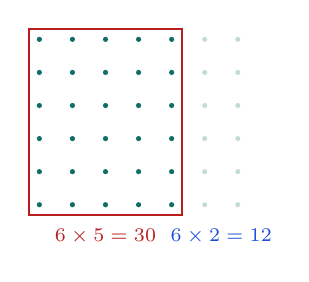
\begin{tikzpicture}[scale=0.42]
          \foreach \x in {0,...,6}{\foreach \y in {0,...,5}{
            \fill[mainc!25] (\x,\y) circle (2.2pt);}}
          \foreach \x in {0,...,4}{\foreach \y in {0,...,5}{
            \fill[mainc] (\x,\y) circle (2.2pt);}}
          \draw[pitc,thick] (-0.32,-0.32) rectangle (4.32,5.32);
          \node[pitc,below,font=\scriptsize] at (2,-0.45) {$6\times5=30$};
          \node[sayc,below,font=\scriptsize] at (5.5,-0.45) {$6\times2=12$};
        \end{tikzpicture}
        \end{center}
        （6 行 7 列，先把左边 5 列框出来。）
  \item \textbf{拆法二：拆成 6 和 1}：$6\times7 = 6\times6 + 6\times1 = 36+6=42$。
  \item \textbf{拆法三：反过来}：$6\times7 = 7\times6$（等 7 的口诀学完就能用）。
  \item \textbf{做四道拆数题，先画图再算}：
        \begin{enumerate}[label=（\arabic*）,itemsep=2pt]
          \item $6\times8 = 6\times5 + 6\times$ \blank[1cm] $=$ \blank[1.4cm]
          \item $6\times9 = 6\times$ \blank[1cm] $+ 6\times$ \blank[1cm] $=$ \blank[1.4cm]
          \item $8\times8 = 8\times$ \blank[1cm] $+ 8\times$ \blank[1cm] $=$ \blank[1.4cm]
          \item $7\times7 = 7\times$ \blank[1cm] $- 7\times$ \blank[1cm] $=$ \blank[1.4cm]
        \end{enumerate}
        答案：（1）3；48\quad（2）如 $6\times5+6\times4=54$\quad
        （3）如 $8\times4+8\times4=64$\quad（4）如 $7\times8-7\times1=49$。
  \item \textbf{收一句贴桌上}：“\textbf{忘了就拆，拆成两句会的加起来。}”
        \textbf{会拆的小豆角永远不会被一句口诀卡死。}
\end{enumerate}

\begin{saybox}
“$6\times7$ 忘了，小豆角能用会的算出来吗？怎么拆？”\\
“为什么可以拆？”（7 列可以分成 5 列加 2 列，点子一个没少）\\
“第 4 题为什么要减？”（多算了 1 个 7，得减掉）
\end{saybox}

\begin{passbox}
\begin{itemize}
  \item 能用两种不同的拆法算出 $6\times7$。
  \item 四道拆数题全对，都能画出图说明。
\end{itemize}
\end{passbox}
\end{lesson}

\subsection{任务 3：7、8、9 的口诀（西游记里全是口诀）}

\begin{lesson}{3}{20}
\textbf{今天要拿下的}：编出 7、8、9；用《西游记》的故事帮着记。

\begin{materials}
百数表、笔、纸。
\end{materials}

\begin{enumerate}
  \item \textbf{先讲三个故事}（课本 P79）：
        \begin{itemize}
          \item 孙悟空有\textbf{八九七十二}般变化；
          \item 在炼丹炉里炼了\textbf{七七四十九}天，炼出火眼金睛；
          \item 唐僧取经经历\textbf{九九八十一}难。
        \end{itemize}
        \textbf{先给这三句}，让小豆角觉得口诀是有来处的，不是凭空一堆字。
  \item \textbf{编 7}（每次加 7）：一七得七、二七十四、三七二十一、四七二十八、
        五七三十五、六七四十二、七七四十九、七八五十六、七九六十三。
  \item \textbf{编 8}（每次加 8）：一八得八、二八十六、三八二十四、四八三十二、
        五八四十、六八四十八、七八五十六、八八六十四、八九七十二。
  \item \textbf{编 9}（每次加 9）：一九得九、二九十八、三九二十七、四九三十六、
        五九四十五、六九五十四、七九六十三、八九七十二、九九八十一。
  \item \textbf{交叉找“双胞胎”}（这一步能省掉一半力气）：
        \begin{center}
        \small
        \begin{tabular}{@{}ll@{}}
        \toprule
        \textbf{得数} & \textbf{对应口诀} \\
        \midrule
        12 & 二六十二、三四十二（两句） \\
        18 & 三六十八、二九十八（两句） \\
        24 & 四六二十四、三八二十四（两句） \\
        36 & 六六三十六、四九三十六（两句） \\
        42 & 六七四十二 \quad 48：六八四十八 \\
        54 & 六九五十四 \quad 56：七八五十六 \\
        63 & 七九六十三 \quad 72：八九七十二 \\
        \bottomrule
        \end{tabular}
        \end{center}
        \textbf{重点盯那四组“双胞胎”}（12、18、24、36），考试最容易混的就是它们。
  \item \textbf{背的顺序别从 1 背到 9}：先背\textbf{平方数}
        （六六三十六、七七四十九、八八六十四、九九八十一），
        它们是锚点，其余靠加减一个推。
\end{enumerate}

\begin{saybox}
“孙悟空会几变？”（七十二变 $\to$ 八九七十二）\\
“哪个得数有两句口诀？找出三组。”\\
“小豆角觉得先记住哪几句最省事？”（平方数）
\end{saybox}

\begin{passbox}
\begin{itemize}
  \item 7、8、9 的口诀能独立编出来（可看表）。
  \item 能找出至少三组“得数相同的两句口诀”。
\end{itemize}
\end{passbox}
\end{lesson}

\subsection{任务 4：9 的口诀，用十根手指}

\begin{lesson}{4}{20}
\textbf{今天要拿下的}：用手指记住 9 的口诀；理解 $9\times n = 10n-n$。

\begin{materials}
小豆角自己的两只手。不用别的。
\end{materials}

\begin{enumerate}
  \item \textbf{手指法}（课本 P80）：
        \begin{center}
        \begin{tikzpicture}[x=0.62cm,y=1cm,font=\scriptsize]
          \foreach \i in {1,...,10}{
            \pgfmathsetmacro{\xx}{\i-1}
            \ifnum\i=4
              \draw[pitc,thick] (\xx,0) -- (\xx,0.45);
              \draw[pitc,thick] (\xx,0.95) -- (\xx,1.4);
            \else
              \draw[tipc,thick] (\xx,0) -- (\xx,1.4);
            \fi
            \node[below] at (\xx,-0.08) {\i};
          }
          \node[pitc,above=2mm] at (3,1.4) {弯下第 4 根};
          \node[mainc] at (1,1.75) {左边 3 根 $\to$ 30};
          \node[mainc] at (6.2,1.75) {右边 6 根 $\to$ 6};
          \node[tipc] at (4.6,2.35) {\textbf{$9\times4=36$}};
        \end{tikzpicture}
        \end{center}
        \textbf{做法}：伸出十指。算 $9\times n$，\textbf{从左往右数，弯下第 $n$ 根}。
        弯下去那根\textbf{左边剩几根，就是十位}；\textbf{右边剩几根，就是个位}。
  \item \textbf{当场验四次}：$9\times2$（弯第 2 根 $\to$ 1 和 8 $\to$ 18）、
        $9\times6$（$\to$ 5 和 4 $\to$ 54）、$9\times7$（$\to$ 63）、$9\times9$（$\to$ 81）。
        \textbf{让小豆角自己弯、自己数。}
  \item \textbf{更好用的规律}：$9\times n = 10n-n$。
        $9\times1=10-1=9$；$9\times2=20-2=18$；$9\times3=30-3=27$……
        让小豆角填完 $9\times5$ 到 $9\times9$：$45$、$54$、$63$、$72$、$81$。
  \item \textbf{第三个规律}：9 的口诀，\textbf{十位加个位都等于 9}
        （18、27、36、45、54、63、72、81）。而且十位 1 到 8 往上走，
        个位 8 到 1 往下走。\textbf{三个规律对三遍，9 的口诀基本不用背了。}
  \item \textbf{往表外推}（课本 P80 试一试）：$9\times10=?$ 用 $90-10=80$；
        $9\times11=9\times10+9=99$。
        \textbf{这说明口诀的规律是能一直往后用的}，不是死表。
\end{enumerate}

\begin{saybox}
“弯第 6 根，左边几根右边几根？”\\
“$9\times n$ 除了手指，还能怎么算？”（$10n-n$）\\
“9 的口诀得数，十位加个位等于几？”（全是 9）
\end{saybox}

\begin{pitbox}
\textbf{手指法的两个坑}：
\begin{enumerate}[label=\arabic*、]
  \item \textbf{从右手开始数}。必须\textbf{从左往右}（左手拇指是第 1 根）。
  \item \textbf{数错边}。提醒：“弯指\textbf{左边当十，右边当个}。”
        练的时候让小豆角\textbf{小声念出来}：“左边 3，30；右边 6，6。”
\end{enumerate}
\end{pitbox}

\begin{passbox}
\begin{itemize}
  \item 手指法能当场算出 9 的任意一句，左右不分错。
  \item 能说出“十位加个位都等于 9”。
  \item 能算出 $9\times10$、$9\times11$。
\end{itemize}
\end{passbox}
\end{lesson}

\subsection{任务 5：收成一张乘法表}

\begin{lesson}{5}{20}
\textbf{今天要拿下的}：45 句收成一张表，并且能从表里看出规律。

\begin{materials}
附录 B 的乘法表（填空版）、彩笔。
\end{materials}

\begin{enumerate}
  \item \textbf{填表}：用填空版，把乘数和积都填上。
        \textbf{这一课主要工作就在这儿，慢点没关系。}
  \item \textbf{一条一条看规律}（课本 P84 的问题）：
        \begin{itemize}
          \item \textbf{对角线}上是什么？（$1\times1$、$2\times2$……$9\times9$，全是平方数）
          \item \textbf{对称吗}？$3\times7$ 和 $7\times3$ 在哪？得数一样吗？（关于对角线对称）
          \item 每一\textbf{行}有什么规律？（第 3 行每次加 3，第 7 行每次加 7）
          \item 每一\textbf{列}呢？
          \item 哪几个得数出现两次？（12、18、24、36）
        \end{itemize}
  \item \textbf{找积是 18 的算式}（课本 P83）：$2\times9$、$3\times6$、$6\times3$、$9\times2$，
        四个算式、两句口诀。
  \item \textbf{找乘数里有 3 的算式}：$3\times1$ 到 $3\times9$，加 $1\times3$ 到 $9\times3$。
  \item \textbf{用表查}：随便报一个数（比如 56），让小豆角在表里找到位置，说出哪句口诀。
        \textbf{这一步是把表当工具用，不是当图片看。}
\end{enumerate}

\begin{saybox}
“表里哪一句最难记？单独做张卡片。”\\
“$3\times7$ 和 $7\times3$ 关于什么对称？”\\
“56 是哪句口诀？在表里指给豆角爸爸看。”
\end{saybox}

\begin{passbox}
\begin{itemize}
  \item 填空版乘法表独立填完，对 90\% 以上。
  \item 能说出三条规律（对角线、对称、每行加几）。
\end{itemize}
\end{passbox}
\end{lesson}

\subsection{任务 6：口诀总过关}

\begin{lesson}{6}{20}
\textbf{今天要拿下的}：横着、竖着、跳着都能答；给一个积能反过来说出乘数。

\begin{materials}
附录 A 的乘法卡、错题卡片。
\end{materials}

\begin{enumerate}
  \item \textbf{三遍法}（每遍 3 分钟，中间歇 1 分钟）：
        \begin{enumerate}[label=第\arabic*遍：]
          \item \textbf{横着}：1 的口诀到 9 的口诀，一行一行过。
          \item \textbf{竖着}：一一得一、一二得二、一三得三……到一九得九；
                再二二得四、二三得六……（按列走，难度高一档）
          \item \textbf{跳着}：豆角爸爸随便报（七八、四九、三六、五八），小豆角报得数。
        \end{enumerate}
  \item \textbf{错的做卡}：跳着背时答错的 3--5 句写卡片，贴镜子或书桌。
        \textbf{只贴错的，不贴整表。}
  \item \textbf{60 秒速算}：抽卡，60 秒对 30 张算过。
  \item \textbf{反着用}：报一个积（42）问“42 除以 6 是几？”$\to$ 想“六七四十二” $\to$ 7。
        \textbf{这是第八单元的前置能力。}
  \item \textbf{打钩}：在附录 D 的进度表上打钩。这一关过了，整册的乘法就稳了。
\end{enumerate}

\begin{passbox}
\begin{itemize}
  \item 跳着问 20 句，对 18 句以上。
  \item 60 秒对 30 张卡。
  \item 给积能立刻说出两个乘数（如 42 $\to$ 6 和 7）。
\end{itemize}
\end{passbox}
\end{lesson}

\subsection{翻车现场（对着看）}

\begin{center}
\small
\begin{tabularx}{\linewidth}{@{}p{3.8cm}p{4.0cm}X@{}}
\toprule
\textbf{小豆角写出来的样子} & \textbf{其实是想错了什么} & \textbf{豆角爸爸回一句什么} \\
\midrule
七八五十六和六七四十二混 & 数字挨着，靠模糊记忆 & 做成两张卡并排看：42 和 56 差 14。\\
\addlinespace[2pt]
9 的手指法左右错 & 从右手数起 & 一律从左往右，弯指左边当十。\\
\addlinespace[2pt]
只会顺着背，倒着问就卡 & 靠顺序记的 & 抽查必须跳着问、倒着问。\\
\addlinespace[2pt]
忘一句就放弃 & 不会拆数 & 拆成两句会的：$6\times7=30+12$。\\
\addlinespace[2pt]
$9\times6$ 答成 56 & 和 $7\times8$ 混了 & 用 $60-6=54$ 验一遍。\\
\addlinespace[2pt]
表填完就不看了 & 只当练习用 & 问“对角线是什么”“关于什么对称”。\\
\bottomrule
\end{tabularx}
\end{center}

\subsection{抽查：随机开枪（10 题）}

\begin{enumerate}[label=\arabic*.,itemsep=4pt]
  \item 六七 \blank[1.6cm] \qquad 2. 七八 \blank[1.6cm] \qquad 3. 九六 \blank[1.6cm]
  \item $7\times8=$ \blank[1.4cm] \qquad 5. $9\times6=$ \blank[1.4cm] \qquad
  6. $8\times8=$ \blank[1.4cm]
  \item $9\times7=$ \blank[1.4cm] \qquad 8. $6\times9=$ \blank[1.4cm]
  \item $42\div6=$ \blank[1.4cm] \qquad 10. $56\div7=$ \blank[1.4cm]
\end{enumerate}

\begin{ansbox}
1. 四十二\quad 2. 五十六\quad 3. 五十四\quad 4. 56\quad 5. 54\quad
6. 64\quad 7. 63\quad 8. 54\quad 9. 7\quad 10. 8 \\
\textbf{第 9、10 题错}：口诀还不能反着用，先专门练“给积说乘数”。
\end{ansbox}

\subsection{课后野路子}

\begin{itemize}
  \item \textbf{每天 3 分钟抽卡}：抽 20 张，跳出来的立刻翻出来单练。
  \item \textbf{饭前对口令}：豆角爸爸一句小豆角一句，跳着来，两分钟。
  \item \textbf{生活里的 6--9}：一盒鸡蛋 3 排 2 列、一箱牛奶 4 排 3 列、
        一层楼 9 级台阶走 7 层。
  \item \textbf{扑克牌}：抽两张相乘，比谁算得快；三张时先乘再加（3、4、5 $\to 3\times4+5$）。
  \item \textbf{买东西}：一包 8 块，买 7 包多少钱？先口令诀再说钱数。
\end{itemize}

% =============================================================
%  第八单元  乘除法的应用（一）
% =============================================================
\Chapter{第八关\quad 算账的本事}
\noindent{\small\kaishu\color{tipc}（课本第八单元：乘除法的应用（一），P87--P93）}

\begin{blunder}
超市结账，收银员说“一共 78”。爸爸扫了码就走，回家对单子才发现：
多扫了一件 9 块的东西，是爸爸自己放进袋子的。
没人提醒，是爸爸自己对着小票一项一项点出来的。
——从那以后，爸爸买东西必对小票。
\end{blunder}

\begin{gamble}{课前协商：二十块预算}
\begin{itemize}
  \item 给小豆角 50 块，让小豆角在超市自己买三样东西，\textbf{自己算够不够}。
  \item 超支了怎么办、省下来的归谁，现在就谈定。
  \item 第二次玩的时候加一条：\textbf{必须买一样“给别人的”}（给妈妈、给爷爷）。
        小豆角会开始算“留给别人的那部分”，这比任何应用题都难。
\end{itemize}
\negolines
\end{gamble}

\begin{bonus}
\begin{itemize}
  \item \textbf{当一天家庭采购员}：给小豆角 50 块，全权负责买今天的菜或水果。
        \textbf{爸爸全程不插嘴}，只在最后问一句“还剩几块？为什么剩这么多？”
  \item \textbf{猜总价}：结账前两人各估一个总价，谁接近谁赢，赢的人记一颗星。
  \item \textbf{36 元挑战}：给小豆角 36 块，让小豆角用“同一种商品”正好花完
        （可以买单价 3、4、6、9、12 的东西）。这题能玩很久。
\end{itemize}
\end{bonus}

\begin{unitinfo}
\textbf{课本 P87--P93}\quad \textbf{4 次课，每次 20 分钟} \\[4pt]
\textbf{这一关到底在干嘛}：前面学的乘和除，这一章全拿来解决真问题。\\
\textbf{逻辑是这么走的}：\ 先判断“知道什么、求什么” $\to$ 判断用乘还是除
$\to$ 想口诀 $\to$ 写算式加单位加答语 $\to$ 用乘法验一遍。\\
\textbf{一个新增难点}：“括号里最大能填几”（$4\times(\ )<18$）。
这个不用新知识，就是\textbf{试乘}——试到刚好不超过为止。
\end{unitinfo}

\subsection{开局先聊个事：这些就是生活里的算账}

长颈鹿造房子，一间用 7 块木板，63 块能造几间？
小鸟住房，6 只住一间，42 只要几间？
——这就是\textbf{知道总数，求能分几份}，用除法。

柿子 54 个，每盒装 6 个，装几盒？
——还是一样。

反过来，5 盒能装多少个？——这是\textbf{知道一份和份数，求总数}，用乘法。

\textbf{生活里算账，来回就这两个方向。}判断对了，剩下就是口诀的事。

\subsection{任务 1：先判断，再动笔}

\begin{lesson}{1}{20}
\textbf{今天要拿下的}：一看到题，先能判断用乘还是用除，说得出理由。

\begin{materials}
纸、笔、小棒（不确定时可以摆）。
\end{materials}

\begin{enumerate}
  \item \textbf{两道题一起出}（课本 P87 长颈鹿与小鸟）：
        \begin{itemize}
          \item \textbf{A}：一间房要 7 块木板，一共 63 块，能造几间？
                $\to 63\div7=9$（间），口诀“七九六十三”
          \item \textbf{B}：42 只小鸟，每 6 只住一间，要几间？
                $\to 42\div6=7$（间），口诀“六七四十二”
        \end{itemize}
        \textbf{两题都是除法}：知道总数，求“能分成几份”。
  \item \textbf{追问（课本 P88）}：造了 9 间，住了 7 间，还有几间空房？
        $9-7=2$（间）。还能住几只？$2\times6=12$（只）。
        \textbf{一道题里乘、除、减都用上了}——这就是“综合”。
  \item \textbf{每题旁边写口诀}。\textbf{写不出口诀，说明是猜的。}
  \item \textbf{只判断，不算（30 秒六道）}：
        \begin{enumerate}[label=（\arabic*）,itemsep=2pt]
          \item 每盒 8 个，5 盒一共多少个？（乘）
          \item 40 个苹果，每盒 8 个，装几盒？（除）
          \item 40 个苹果，平均装 5 盒，每盒几个？（除）
          \item 一班 35 人，7 人一组，分几组？（除）
          \item 每排 7 人，5 排一共多少人？（乘）
          \item 一支笔 6 元，5 支多少元？（乘）
        \end{enumerate}
  \item \textbf{四步法再走一遍}：圈数字 $\to$ 说关系 $\to$ 想口诀 $\to$
        写算式＋单位＋答语。
\end{enumerate}

\begin{saybox}
“这题知道总数吗？知道每份几个吗？那求什么？”\\
“小豆角用的是哪句口诀？”\\
“算出来是‘间’还是‘只’？念一遍问题再写单位。”
\end{saybox}

\begin{passbox}
\begin{itemize}
  \item 六道判断题全对。
  \item 两道应用题的算式、口诀、单位、答语都齐。
\end{itemize}
\end{passbox}
\end{lesson}

\subsection{任务 2：括号里最大能填几}

\begin{lesson}{2}{20}
\textbf{今天要拿下的}：会用“试乘”解决 $4\times(\ )<18$，并且知道填完要验。

\begin{materials}
小棒 18 根、纸、笔。
\end{materials}

\begin{enumerate}
  \item \textbf{给情境}（课本 P88）：18 只小松鼠分组，每组只数一样。
        每组 4 只，\textbf{最多}分几组？
  \item \textbf{先摆}：18 根小棒，4 根一堆。堆 4 堆用掉 16 根，还多 2 根——
        \textbf{不够再堆一堆}。所以最多 4 组。
  \item \textbf{写成算式}：$4\times(\ )<18$，括号里最大填几？
        \begin{itemize}
          \item 试乘：$4\times4=16$（小于 18，行）；$4\times5=20$（超过 18，不行）
          \item 所以最大填 \textbf{4}。
        \end{itemize}
  \item \textbf{第二种办法（用除法）}：$18\div4$——想“四五二十”太大、
        “四四十六”合适，商 4，剩 2。所以填 4。
        \textbf{两种办法都教，小豆角挑顺手的用。}
  \item \textbf{连做八道}（课本 P89）：
        \begin{center}
        \small
        \begin{tabular}{@{}llll@{}}
        $8\times(\ )<70$ & $6\times(\ )<29$ & $9\times(\ )<50$ & $(\ )\times9<55$ \\
        $(\ )\times7<65$ & $(\ )\times5<48$ & $5\times(\ )<36$ & $8\times(\ )<39$ \\
        \end{tabular}
        \end{center}
        答案：8、4、5、6、9、9、7、4。
  \item \textbf{易错对比}：$8\times(\ )<70$ 为什么不是 9？
        （$8\times9=72$，比 70 大，不行）——\textbf{填完必须乘一遍验}。
  \item \textbf{小兔安家}（课本 P89）：24 只小兔。
        \begin{center}
        \small
        \begin{tabular}{@{}lcccc@{}}
        \toprule
        每间住几只 & 4 & 6 & 3 & 8 \\
        \midrule
        需要几间 & \blank[1cm] & \blank[1cm] & \blank[1cm] & \blank[1cm] \\
        \bottomrule
        \end{tabular}
        \end{center}
        答案：6、4、8、3。\textbf{顺便发现}：每间住得越多，需要的间数越少。
\end{enumerate}

\begin{saybox}
“$4\times5=20$，20 比 18 大还是小？能填 5 吗？”\\
“除了一个个试，还能怎么想？”（用除法：$18\div4$）\\
“填完小豆角怎么确认它对？”（乘一遍，看有没有超过右边）
\end{saybox}

\begin{pitbox}
\textbf{最常见的错}：填了一个让乘积\textbf{超过}右边数的值
（比如 $8\times(\ )<70$ 填 9）。\\
\textbf{解法}：\textbf{这类题填完必须乘一遍}。
养成“填完就验”，比多做十道题有用。
\end{pitbox}

\begin{passbox}
\begin{itemize}
  \item 八道全对，\textbf{每道都有验算痕迹}。
  \item 能用两种办法（试乘 / 用除法）解同一道。
\end{itemize}
\end{passbox}
\end{lesson}

\subsection{任务 3：一页图里全是应用}

\begin{lesson}{3}{20}
\textbf{今天要拿下的}：同一幅图里把乘、除、倍、加减都用一遍。

\begin{materials}
课本 P90 农家小院、笔。
\end{materials}

\begin{enumerate}
  \item \textbf{先读图说话}：让小豆角把图里能看到的数学信息\textbf{全说出来}：
        柿子 54 个、每盒装 6 个、墙上的玉米、兔子、豇豆 42 厘米、扁豆 7 厘米……
        \textbf{这一步叫“读图”。考试里八成的错，是因为信息没读全就开始写。}
  \item \textbf{逐题解决}（每题都走四步法）：
        \begin{enumerate}[label=（\arabic*）,itemsep=3pt]
          \item 54 个柿子，每盒 6 个，装几盒？$54\div6=9$（盒）
          \item 豇豆 42 厘米，扁豆 7 厘米，豇豆是扁豆的几倍？$42\div7=6$（倍）
          \item 平均每个笼子住几只兔子？（让小豆角自己数出两个数再列式）
          \item 可以装几筐？（看每筐装几个）
        \end{enumerate}
  \item \textbf{接着追问}（课本 P91）：
        \begin{itemize}
          \item 多少个柿子刚好装满 5 盒？$6\times5=30$（个）——\textbf{这是乘法}
          \item 已经摘了 30 个，树上还剩多少？$54-30=24$（个）
          \item 剩下 24 个还能装几盒？$24\div6=4$（盒）
        \end{itemize}
        \textbf{一道题，乘、减、除连着用。}这就是这一章的核心。
  \item \textbf{自己提问题}：让小豆角看图提两个用乘法的、两个用除法的，写下来并解答。
  \item \textbf{36 元能买什么}（课本 P91）：给 3、4、5、6、7、9 元几种商品，
        “李老师买了同一种商品正好花 36 元，可能买了什么？买了多少？”
        \textbf{答案不止一个}：9 元的买 4 个、6 元的买 6 个、4 元的买 9 个、
        3 元的买 12 个。\textbf{让小豆角尽量多找几种}，这是很好的发散练习。
\end{enumerate}

\begin{saybox}
“图里一共有哪些数字？都找全了吗？”\\
“这道为什么用乘法不用除法？”\\
“36 元还能买什么？再想一种。”\\
“单位写了吗？答语写了吗？”
\end{saybox}

\begin{passbox}
\begin{itemize}
  \item 能说全图里的信息（至少六条）。
  \item 四道题算式对、单位对、答语完整。
  \item “36 元”那题能找出三种以上买法。
\end{itemize}
\end{passbox}
\end{lesson}

\subsection{任务 4：自己编题 + 综合过关}

\begin{lesson}{4}{20}
\textbf{今天要拿下的}：给算式能编出生活问题；一道综合题从头做到尾。

\begin{materials}
纸、笔、错题本。
\end{materials}

\begin{enumerate}
  \item \textbf{给算式编事}（每次 1 分钟，编四个）：
        $7\times8=56$、\ $48\div6=8$、\ $36\div9=4$、\ $9\times7=63$。
        \textbf{要求人物、东西、单位都对得上。}
        （“48 颗糖，每 6 颗装一袋，能装 8 袋。”）
  \item \textbf{反过来}：爸爸说一个生活情境，小豆角写算式（五个）。
  \item \textbf{综合过关题}：
        \begin{tipbox}
        学校要给 6 个班每班发 7 本图书。\\
        （1）一共需要多少本？\\
        （2）图书角现在有 40 本，够吗？还差几本？\\
        （3）学校又买来 8 本，现在一共 48 本，平均分给 8 个小组，每组几本？
        \end{tipbox}
        答案：（1）$6\times7=42$（本）；
        （2）$42-40=2$（本），\textbf{不够，还差 2 本}；
        （3）$48\div8=6$（本）。
  \item \textbf{整理错题}：把本单元和前面各单元快检的错题看一遍，
        挑出\textbf{同一个错因出现三次以上}的，那就是期末重点补的地方。
\end{enumerate}

\begin{passbox}
\begin{itemize}
  \item 四个算式都能编出合理的故事（人、物、单位都对）。
  \item 综合题三步全对。
\end{itemize}
\end{passbox}
\end{lesson}

\subsection{翻车现场（对着看）}

\begin{center}
\small
\begin{tabularx}{\linewidth}{@{}p{3.8cm}p{4.0cm}X@{}}
\toprule
\textbf{小豆角写出来的样子} & \textbf{其实是想错了什么} & \textbf{爸爸回一句什么} \\
\midrule
$8\times(\ )<70$ 填 9 & 没验算 & 填完必须乘一遍。 \\
\addlinespace[2pt]
不知道用乘还是除 & 没先判断“知道什么、求什么” & 走四步法：圈 → 说 → 想 → 写。 \\
\addlinespace[2pt]
单位写“个”其实该写“盒” & 没回头读问题 & 写完念一遍问的是什么。 \\
\addlinespace[2pt]
答语只写个数字 & 书写习惯 & “答：……。”一整句写出来。 \\
\addlinespace[2pt]
除法不验算 & 没检查习惯 & 商 $\times$ 除数 $=$ 被除数。 \\
\addlinespace[2pt]
图里的信息没读全 & 看图太快 & 先“说出来”，再动笔。 \\
\bottomrule
\end{tabularx}
\end{center}

\subsection{抽查：随机开枪（10 题）}

\begin{enumerate}[label=\arabic*.,itemsep=4pt]
  \item $63\div7=$ \blank[1.4cm] \qquad 2. $42\div6=$ \blank[1.4cm] \qquad
  3. $54\div6=$ \blank[1.4cm]
  \item $8\times(\ )<70$，最大填 \blank[1.4cm]。
  \item $9\times(\ )<50$，最大填 \blank[1.4cm]。
  \item 每间房住 6 只小鸟，42 只要 \blank[1.4cm] 间。
  \item 63 块木板，每间用 7 块，能造 \blank[1.4cm] 间。
  \item 豇豆 42 厘米，扁豆 7 厘米，豇豆是扁豆的 \blank[1.4cm] 倍。
  \item 每盒 6 个，9 盒一共 \blank[1.4cm] 个。
  \item 54 个柿子，每盒 6 个，装 \blank[1.4cm] 盒。
\end{enumerate}

\begin{ansbox}
1. 9\quad 2. 7\quad 3. 9\quad 4. 8\quad 5. 5\quad 6. 7\quad
7. 9\quad 8. 6\quad 9. 54\quad 10. 9 \\
\textbf{全对} $\to$ 可以进期末复习。\textbf{错两题以上} $\to$ 回对应的课补 20 分钟。
\end{ansbox}


% ---------- 综合实践 ----------
% =============================================================
%  综合实践：两次必须动手的活动
% =============================================================
\Chapter{隐藏关\quad 画地图，花真钱}
\noindent{\small\kaishu\color{tipc}（课本两次综合实践：画校园路线图 P53--P55；欢乐购物 P94--P97）}

\begin{blunder}
带小豆角去商场，找厕所绕了三圈。最后是小豆角指着一块指示牌说：
“爸爸，刚才爸爸和小豆角是从那边过来的。”
——一个小孩的方向感比爸爸好，这事豆角爸爸认了。
\end{blunder}

\begin{gamble}{课前协商：藏宝图}
\begin{itemize}
  \item 小豆角画一张家里的“藏宝图”，标上东南西北，把一样他自己挑的东西藏起来。
  \item \textbf{豆角爸爸只能看小豆角的图去找}，不许开口问。
  \item 找到了归谁、找不到归谁，写在下面；但要小豆角说清“图上哪儿画错了”。
\end{itemize}
\negolines
\end{gamble}

\begin{bonus}
\begin{itemize}
  \item \textbf{跳蚤市场}：把家里闲置的小玩具、旧绘本摆摊卖掉，
        \textbf{赚的钱全归小豆角}。定价、算钱、找零，全小豆角自己来。
  \item \textbf{给爸爸画一张“到暖暖家怎么走”}：不许写地址，只许画图加方向。
        爸爸真按图走一次，能不能找到门？
  \item \textbf{超市寻宝}：拿手机指南针，只给三条线索（“往北走三个货架”“在收银台西边”），
        让小豆角自己找一件指定的东西。
\end{itemize}
\end{bonus}

\begin{unitinfo}
课本里安排了两次综合实践，一共占 5 页。这不是装饰——
\textbf{期末卷里的“方向”和“人民币”，几乎全从这两课出}。\\
\textbf{活动一}：画一张能用的路线图（学完第四单元后做，40 分钟）\\
\textbf{活动二}：真刀真枪买东西（学完第八单元后做，60 分钟）
\end{unitinfo}

\subsection{活动一：认方向，然后画一张真能用的图}

\begin{lesson}{1}{40}
\textbf{今天要拿下的}：认得出东南西北；画的图别人拿着能找得到地方。

\begin{materials}
手机（开指南针）、A3 纸或两张 A4 拼起来、铅笔、直尺。
\end{materials}

\begin{enumerate}
  \item \textbf{先在屋里认四个方向}：
        \begin{itemize}
          \item 打开手机指南针，找到\textbf{北}。让小豆角站在客厅中间，面向北。
          \item 教一句口诀：\textbf{面朝北，背后是南，左手是西，右手是东}。
          \item 让小豆角原地转圈，每转 90° 说一个方向。
          \item \textbf{考小豆角四道}：“小豆角面向南，左手是哪边？”（东）
        \end{itemize}
  \item \textbf{到小区里实地走 15 分钟}：从家门口出发，往北走 30 米看看有什么，
        再往东走看看有什么。\textbf{边走边在纸上记}：
        “北：小卖部；东：篮球场；南：大门；西：花坛”。
        \textbf{必须真走，不能坐桌边编。}
  \item \textbf{画图（重点）}：
        \begin{enumerate}[label=第\arabic*步：]
          \item 在纸的\textbf{右上角}画一个“北”箭头（\tikz[baseline=-0.6ex]{\draw[tipc,thick,->](0,0)--(0,0.5);} 朝上）。
                \textbf{这一步不画，整张图作废，考试也要扣分。}
          \item 定一个中心点（家／大门），画它四周的建筑。
          \item 用箭头把“从门口到目标地点”的路线画出来。
          \item 目标地点打一个 \textbf{▲}，写上名字。
        \end{enumerate}
        两条规则：\textbf{上北下南、左西右东}。
  \item \textbf{验收}：让家里另一个人只看这张图去找那个地方。
        \textbf{找到了，图才算合格}；找不到，问小豆角“小豆角哪儿没看懂”，回去改。
  \item \textbf{补中间方向}（课本 P55 的问题）：“种植园在西和南之间，画在哪？”
        （\textbf{西南角}）让小豆角把西南、东南、东北、西北四个角都标出来。
\end{enumerate}

\begin{saybox}
“小豆角面向北，左手是哪边？”\\
“为什么要把‘北’画在上面？”\\
“其他人拿着这张图能找到地方吗？小豆角哪儿没看懂？”
\end{saybox}

\begin{passbox}
\begin{itemize}
  \item 能说出“面朝北，左手西，右手东”，并推得出别的朝向。
  \item 画出的图有方向标、有建筑、有箭头，别人照着能找到。
\end{itemize}
\end{passbox}
\end{lesson}

\subsection{活动二：真刀真枪买东西}

\begin{lesson}{2}{60}
\textbf{今天要拿下的}：认得钱、会换钱、会算找零，并且在真买卖里把乘除加减用一遍。

\begin{materials}
附录 C 的模拟人民币（卡纸印好剪开）、家里小物件 8--10 件
（玩具、本子、橡皮、零食）、价格标签纸、笔、两张记录表。
\end{materials}

\begin{enumerate}
  \item \textbf{认钱（10 分钟）}：
        \begin{itemize}
          \item 把剪好的钱摊开，让小豆角说出每一张的面值和单位。
          \item \textbf{记住换算}：\ $1\ \text{元}=10\ \text{角}$，\ $1\ \text{角}=10\ \text{分}$。
          \item \textbf{换钱五道}（口答）：1 元换几张 5 角？10 元换几张 1 元？
                5 元换几张 5 角？2 元 5 角是多少角？38 角是几元几角？
                答案：2、10、10、25、3 元 8 角。
        \end{itemize}
  \item \textbf{给东西定价（10 分钟）}：让小豆角自己给每件东西定价，
        \textbf{要求是整元或“X 元 5 角”}。定价时想三件事：新旧、原来多少钱、
        小朋友买得起吗。
        \begin{center}
        \small
        \begin{tabular}{@{}p{4cm}p{3cm}p{3cm}p{3cm}@{}}
        \toprule
        \textbf{豆角爸爸卖的} & \textbf{原价} & \textbf{豆角爸爸定的价} & \textbf{卖掉了吗} \\
        \midrule
        \blank[3.2cm] & \blank[2.2cm] & \blank[2.2cm] & \blank[2.2cm] \\
        \blank[3.2cm] & \blank[2.2cm] & \blank[2.2cm] & \blank[2.2cm] \\
        \blank[3.2cm] & \blank[2.2cm] & \blank[2.2cm] & \blank[2.2cm] \\
        \blank[3.2cm] & \blank[2.2cm] & \blank[2.2cm] & \blank[2.2cm] \\
        \bottomrule
        \end{tabular}
        \end{center}
        \textbf{让小豆角自己体会}：“定价太高没人买，太低小豆角会亏。”
  \item \textbf{准备零钱（5 分钟）}：让小豆角自己决定每种面值准备几张，
        并算出总额。顺便说出课本那句话：“\textbf{要多准备小面值的，方便找钱}。”
  \item \textbf{正式买卖（20 分钟）——必须真给钱、真找钱}：
        \begin{itemize}
          \item 第一轮：\textbf{小豆角当卖家}，豆角爸爸当买家。豆角爸爸给大票
                （买 7 块的给 10 块），让小豆角算找零。\letgo{豆角爸爸偶尔会把找零算错}，
                看小豆角能不能发现。
          \item 第二轮：\textbf{小豆角当买家}，给小豆角 20 元预算，买三样东西，
                自己算一共多少钱、够不够、该找多少。
        \end{itemize}
        \begin{center}
        \small
        \begin{tabular}{@{}p{2.8cm}p{1.8cm}p{1.8cm}p{1.8cm}p{1.8cm}@{}}
        \toprule
        \textbf{东西} & \textbf{定价} & \textbf{付了} & \textbf{找零} & \textbf{对不对} \\
        \midrule
        \blank[2.4cm] & \blank[1.2cm] & \blank[1.2cm] & \blank[1.2cm] & \blank[1.2cm] \\
        \blank[2.4cm] & \blank[1.2cm] & \blank[1.2cm] & \blank[1.2cm] & \blank[1.2cm] \\
        \blank[2.4cm] & \blank[1.2cm] & \blank[1.2cm] & \blank[1.2cm] & \blank[1.2cm] \\
        \bottomrule
        \end{tabular}
        \end{center}
  \item \textbf{算总账（10 分钟）}：卖出所得加起来，看赚了多少；买花掉的加起来，
        看剩下多少。\textbf{顺手把两位数加减复习一遍。}
  \item \textbf{真去一趟超市（这周内）}：给小豆角 20 元，让小豆角自己买一次东西，
        \textbf{自己算找零}。\textbf{这是本单元最值钱的一次作业}，比十张卷子有用。
  \item \textbf{加点料}（课本 P97）：人民币到现在发行了五套，
        第五套纸币背面分别是西湖三潭印月、泰山、长江三峡、桂林山水、
        布达拉宫、人民大会堂。\textbf{真拿几张出来看看背面。}
\end{enumerate}

\begin{saybox}
“1 元等于几角？那 2 元 5 角呢？”\\
“豆角爸爸给小豆角 10 元，东西 7 元，小豆角该找多少？”\\
“找的零钱对不对？用加法验一下。”（找零 $+$ 货款 $=$ 付出的钱）\\
“定价 60 元，会有人买吗？”
\end{saybox}

\begin{passbox}
\begin{itemize}
  \item 五道换钱全对（包括“38 角 = 3 元 8 角”）。
  \item 能独立完成一次买卖：算总额、算找零、验算对。
  \item 能用 20 元买三样东西并算清剩多少。
\end{itemize}
\end{passbox}
\end{lesson}

\begin{tipbox}
\textbf{两个提醒}：\\
① \textbf{一定要用真钱或仿真币，别在纸上“假装”}。二年级的钱感是摸出来的。\\
② 找零算错时\textbf{别直接说答案}，说“重新数一遍钱”。
把钞票一张张摊开数，比讲道理快十倍。
\end{tipbox}


% ---------- 期末总复习 ----------
% =============================================================
%  期末总复习
% =============================================================
\Chapter{终局\quad 考前三十天}
\noindent{\small\kaishu\color{tipc}（课本总复习 P98--P103）}

\begin{blunder}
豆角爸爸小时候考砸了一次，回家大人说：“没关系。”
正准备松口气，大人从柜子里拿出一套卷子：“趁热打铁，做做。”
——那是豆角爸爸第一次知道什么叫“笑里藏刀”。
所以豆角爸爸这份东西里，\textbf{考前一天只做四件事，一件都不是做新题}。
\end{blunder}

\begin{gamble}{赌一把：模拟卷换钓鱼}
\begin{itemize}
  \item 开考前跟小豆角约好一个分数线（\textbf{别定 100，定 85 就好}）。
  \item 达到了，\textbf{换一次钓鱼机会}；没达到，不罚，但要把错题讲给豆角爸爸听。
  \item \textbf{讲得清就再给一次机会}——因为“讲明白”比“考高分”值钱。
\end{itemize}
\end{gamble}

\begin{bonus}
\begin{itemize}
  \item \textbf{角色反转}：让小豆角当老师，给豆角爸爸出十道题，豆角爸爸答。
        \textbf{豆角爸爸故意错三道}，小豆角必须指出错在哪——小豆角指得出来，说明小豆角真会了。
  \item \textbf{错题拍卖}：把错题本里最难的三道题拿出来，讲对的人赢一颗星。
  \item \textbf{考前“免做题卡”}：连续三天抽查全对，换一张“免做一道题”的卡，
        期末前用掉。小豆角会为了这张卡认真起来。
\end{itemize}
\end{bonus}

\begin{unitinfo}
别等考前一星期才开动。八个单元加两次实践，考前一周搞不完，只能搞得小豆角很慌。\\
\textbf{三轮，每天二十分钟，三周够用}：\\
\textbf{第一轮}——回到八个单元，把每章末尾的“5 分钟快检”重做一遍，找出弱的那个。\\
\textbf{第二轮}——按专项打：计算、口诀、图形测量、应用方向，各来一遍。\\
\textbf{第三轮}——做两套模拟卷，练手感和时间。
\end{unitinfo}

\subsection{三轮怎么排}

\begin{center}
\small
\begin{tabularx}{\linewidth}{@{}p{1.8cm}p{2.6cm}Xp{2.8cm}@{}}
\toprule
\textbf{轮次} & \textbf{什么时候} & \textbf{干什么} & \textbf{每天多久} \\
\midrule
第一轮 & 考前第 3 周前 5 天 & 八章的快检各重做一遍，错的记进错题本，标出最弱的章 &
       20 分钟 \\
第二轮 & 考前第 2 周 & 四个专项各练一次，题在下面 & 20--25 分钟 \\
第三轮 & 考前最后一周 & 模拟卷 A、B 各做一次，讲评一次，最后一天只看错题不做新题 &
       30 分钟 \\
考前那天 & 就这一天 & 只看错题本、背口诀、检查文具，别的都别干 & 15 分钟 \\
\bottomrule
\end{tabularx}
\end{center}

\subsection{第一轮：八个单元过一遍}

做完一章打个钩，错的题号写下来。\textbf{错三道以上的那章，第二轮要重点打。}

\begin{center}
\small
\begin{tabularx}{\linewidth}{@{}p{0.8cm}p{5.4cm}p{1.6cm}X@{}}
\toprule
\textbf{序} & \textbf{哪一章} & \textbf{做完了} & \textbf{错题号 / 备注} \\
\midrule
1 & 100 以内加与减（二） & \cb & \blank[4.4cm] \\
2 & 测量（一） & \cb & \blank[4.4cm] \\
3 & 数一数与乘法 & \cb & \blank[4.4cm] \\
4 & 乘法口诀（一） & \cb & \blank[4.4cm] \\
5 & 分一分与除法 & \cb & \blank[4.4cm] \\
6 & 图形的运动（一） & \cb & \blank[4.4cm] \\
7 & 乘法口诀（二） & \cb & \blank[4.4cm] \\
8 & 乘除法的应用（一） & \cb & \blank[4.4cm] \\
\bottomrule
\end{tabularx}
\end{center}

\subsection{第二轮：四个专项}

\subsubsection{专项一：100 以内加减（含竖式）}
\begin{enumerate}[label=\arabic*.,itemsep=3pt]
  \item $46+38=$ \quad 2. $27+65=$ \quad 3. $9+83=$ \quad 4. $52-27=$ \quad
  5. $80-46=$
  \item $100-58=$ \quad 7. $73-38=$ \quad 8. $35+49=$ \quad 9. $60-24=$ \quad
  10. $91-46=$
\end{enumerate}
\textbf{答案}：1. 84\quad 2. 92\quad 3. 92\quad 4. 25\quad 5. 34\quad
6. 42\quad 7. 35\quad 8. 84\quad 9. 36\quad 10. 45\\
\textbf{要求}：第 6--10 题\textbf{必须写竖式}，进位小 1 和退位点都得有。

\subsubsection{专项二：口诀与乘除计算}
\begin{enumerate}[label=\arabic*.,itemsep=3pt]
  \item $7\times8=$ \quad 2. $6\times9=$ \quad 3. $9\times9=$ \quad 4. $8\times8=$ \quad
  5. $7\times7=$
  \item $54\div6=$ \quad 7. $72\div8=$ \quad 8. $63\div7=$ \quad 9. $45\div5=$ \quad
  10. $36\div9=$
  \item $8\times(\ )<60$，最大填 \blank[1.2cm]。\quad
  12. $(\ )\times7<50$，最大填 \blank[1.2cm]。
\end{enumerate}
\textbf{答案}：1. 56\quad 2. 54\quad 3. 81\quad 4. 64\quad 5. 49\quad
6. 9\quad 7. 9\quad 8. 9\quad 9. 9\quad 10. 4\quad 11. 7\quad 12. 7

\subsubsection{专项三：测量与图形}
\begin{enumerate}[label=\arabic*.,itemsep=3pt]
  \item 填单位：教室长约 8 \blank[1.4cm]；一支新铅笔长约 18 \blank[1.4cm]。
  \item $1\ \text{米}=$ \blank[1.2cm] 厘米；\ $250\ \text{厘米}=$ \blank[1.2cm] 米
        \blank[1.2cm] 厘米。
  \item 一条线段从 3 画到 11，长 \blank[1.2cm] 厘米。
  \item 用坏尺子画 7 厘米，从 5 画到 \blank[1.2cm]。
  \item 下面哪些是轴对称图形？（圆、正方形、平行四边形、等腰三角形、等腰梯形）
  \item 陀螺的轴扎在纸板哪儿转得最稳？
  \item 华容道里的人物，每次只能往哪儿移？
\end{enumerate}
\textbf{答案}：1. 米；厘米\quad 2. 100；2 米 50 厘米\quad 3. 8\quad 4. 12\quad
5. 圆、正方形、等腰三角形、等腰梯形（\textbf{平行四边形不是}）\quad
6. 中心\quad 7. 只能横着或竖着。

\subsubsection{专项四：应用与方向}
\begin{enumerate}[label=\arabic*.,itemsep=3pt]
  \item 每盘 6 个苹果，7 盘一共多少个？
  \item 42 个苹果，每 6 个装一盘，能装几盘？
  \item 小明有 8 张卡片，小红有 32 张，小红是小明的几倍？
  \item 一支笔 5 元，买 7 支多少钱？给 50 元找回多少？
  \item 一本书 9 元，买 6 本，60 元够吗？
  \item 小红面向北，她后面是 \blank[1.2cm]，左面是 \blank[1.2cm]。
  \item 地图上一般是上 \blank[1cm] 下 \blank[1cm] 左 \blank[1cm] 右 \blank[1cm]。
\end{enumerate}
\textbf{答案}：1. $6\times7=42$（个）\quad 2. $42\div6=7$（盘）\quad
3. $32\div8=4$（倍）\quad 4. $5\times7=35$（元），$50-35=15$（元）\quad
5. $9\times6=54$（元），$54<60$ 够\quad 6. 南；西\quad 7. 北、南、西、东。

\subsection{第三轮：模拟卷 A（数与代数）}

\begin{tipbox}
\textbf{做题要求}：一次做完，限时 40 分钟；不会的先跳过，做完再回头；
\textbf{做完小豆角自己先检查一遍}，再给豆角爸爸看。
\end{tipbox}

\noindent\textbf{一、直接写出得数（每题 1 分，共 10 分）}
\begin{enumerate}[label=\arabic*.,itemsep=2pt]
  \item $8\times7=$ \blank[1.4cm] \quad 2. $45\div9=$ \blank[1.4cm] \quad
  3. $36+29=$ \blank[1.4cm] \quad 4. $70-26=$ \blank[1.4cm] \quad
  5. $6\times9=$ \blank[1.4cm]
  \item $54\div6=$ \blank[1.4cm] \quad 7. $100-48=$ \blank[1.4cm] \quad
  8. $7\times8=$ \blank[1.4cm] \quad 9. $24\div4=$ \blank[1.4cm] \quad
  10. $56\div7=$ \blank[1.4cm]
\end{enumerate}

\noindent\textbf{二、用竖式计算（每题 3 分，共 12 分）}
\begin{enumerate}[label=\arabic*.,itemsep=6pt]
  \item $38+27=$ \wls[2]
  \item $100-36=$ \wls[2]
  \item $47+29=$ \wls[2]
  \item $82-45=$ \wls[2]
\end{enumerate}

\noindent\textbf{三、填一填（每空 1 分，共 20 分）}
\begin{enumerate}[label=\arabic*.,itemsep=3pt]
  \item 5 个 6 相加是 \blank[1.4cm]，用乘法算式表示是 \blank[3cm]。
  \item $1\ \text{米}=$ \blank[1.2cm] 厘米；\ $300\ \text{厘米}=$ \blank[1.2cm] 米。
  \item 一支铅笔长约 18 \blank[1.4cm]；教室长约 8 \blank[1.4cm]。
  \item 一个数除以 7 得 8，这个数是 \blank[1.4cm]。
  \item $8\times(\ )<60$，括号里最大填 \blank[1.4cm]。
  \item 12 个苹果平均分给 4 人，每人 \blank[1.2cm] 个；
        如果每人 3 个，可以分给 \blank[1.2cm] 人。
  \item $\triangle\triangle\triangle\triangle$ \ $\triangle\triangle\triangle\triangle$ \
        $\triangle\triangle\triangle\triangle$ 表示 \blank[1cm] 个 \blank[1cm]，
        乘法算式是 \blank[2.6cm]。
  \item 在 $6\times7$ 和 $7\times6$ 中间填 $>$、$<$ 或 $=$：\blank[1.4cm]。
  \item 45 是 9 的 \blank[1.2cm] 倍。
  \item 钟面上有 12 个数，每 3 个数一组，可以分成 \blank[1.2cm] 组。
\end{enumerate}

\noindent\textbf{四、判断（对的打“√”，错的打“×”，每题 1 分，共 5 分）}
\begin{enumerate}[label=\arabic*.,itemsep=2pt]
  \item $3+4$ 可以写成 $3\times4$。\hfill（\quad）
  \item 所有的乘法口诀都能写出两个乘法算式。\hfill（\quad）
  \item 1 米比 100 厘米长。\hfill（\quad）
  \item 求 48 是 6 的几倍，用 $48\div6$。\hfill（\quad）
  \item $100-48=62$。\hfill（\quad）
\end{enumerate}

\noindent\textbf{五、选择（每题 1 分，共 5 分）}
\begin{enumerate}[label=\arabic*.,itemsep=2pt]
  \item 下面哪个数是 7 的倍数？\quad A. 42 \quad B. 45 \quad C. 50 \hfill（\quad）
  \item 小红面向北，她右手边是\quad A. 东 \quad B. 南 \quad C. 西 \hfill（\quad）
  \item 一支笔 3 元，买 6 支要\quad A. 9 元 \quad B. 18 元 \quad C. 2 元 \hfill（\quad）
  \item $25\div5=$\quad A. 4 \quad B. 5 \quad C. 6 \hfill（\quad）
  \item 一根绳子长 2 米，剪去 60 厘米，还剩\quad
        A. 140 厘米 \quad B. 130 厘米 \quad C. 60 厘米 \hfill（\quad）
\end{enumerate}

\noindent\textbf{六、解决问题（每题 7 分，共 28 分）}
\begin{enumerate}[label=\arabic*.,itemsep=8pt]
  \item 每盒装 8 个鸡蛋，买 5 盒一共多少个？
        \wls[2]
  \item 有 36 个苹果，每 4 个装一袋，能装几袋？
        \wls[2]
  \item 小明今年 7 岁，爷爷 63 岁，爷爷的年龄是小明的几倍？
        \wls[2]
  \item 一本书 9 元，小红有 50 元，买 5 本够吗？还剩多少元？
        \wls[3]
\end{enumerate}

\begin{ansbox}
\textbf{卷 A 答案}\\
\textbf{一}：1. 56\quad 2. 5\quad 3. 65\quad 4. 44\quad 5. 54\quad
6. 9\quad 7. 52\quad 8. 56\quad 9. 6\quad 10. 8 \\
\textbf{二}：1. 65\quad 2. 64\quad 3. 76\quad 4. 37 \\
\textbf{三}：1. 30；$5\times6=30$（或 $6\times5=30$）\quad 2. 100；3\quad
3. 厘米；米\quad 4. 56\quad 5. 7\quad 6. 3；4\quad 7. 3 个 4；$3\times4=12$\quad
8. $=$\quad 9. 5\quad 10. 4 \\
\textbf{四}：1. ×\quad 2. ×（四四十六只有一个）\quad 3. ×\quad 4. √\quad
5. ×（应是 52）\\
\textbf{五}：1. A\quad 2. A\quad 3. B\quad 4. B\quad 5. A \\
\textbf{六}：1. $8\times5=40$（个）\quad 2. $36\div4=9$（袋）\quad
3. $63\div7=9$\quad 4. $9\times5=45$（元），$45<50$ 够；$50-45=5$（元），还剩 5 元。
\end{ansbox}

\subsection{模拟卷 B（图形、测量与综合）}

\noindent\textbf{一、填一填（每空 1 分，共 16 分）}
\begin{enumerate}[label=\arabic*.,itemsep=3pt]
  \item 填单位：一张床长约 2 \blank[1.4cm]；一块橡皮厚约 1 \blank[1.4cm]。
  \item $1\ \text{米}=$ \blank[1.2cm] 厘米；\ $180\ \text{厘米}=$ \blank[1.2cm] 米
        \blank[1.2cm] 厘米。
  \item $1\ \text{元}=$ \blank[1.2cm] 角；\ $1\ \text{角}=$ \blank[1.2cm] 分；
        $2\ \text{元}5\ \text{角}=$ \blank[1.2cm] 角。
  \item 地图上一般是上 \blank[1cm]、下 \blank[1cm]、左 \blank[1cm]、右 \blank[1cm]。
  \item 小红面向西，她左手边是 \blank[1.2cm]，右手边是 \blank[1.2cm]。
  \item 正方形纸对折后剪一个图形，展开后两边 \blank[2cm]（填“一样”或“不一样”）。
\end{enumerate}

\noindent\textbf{二、量一量、画一画（每题 4 分，共 12 分）}
\begin{enumerate}[label=\arabic*.,itemsep=6pt]
  \item 量一量家里三样东西的长度，写在下面。
        \wls[2]
  \item 画一条长 5 厘米的线段。
        \wls[3]
  \item 画一条长 7 厘米的线段。
        \wls[3]
\end{enumerate}

\noindent\textbf{三、下面哪些是轴对称图形？在括号里打“√”（每题 2 分，共 10 分）}
\begin{center}
\begin{tikzpicture}[scale=0.62]
  \draw[thick] (0,0) circle (0.7);
  \node[below] at (0,-1.0) {圆（\quad）};
  \draw[thick] (2.1,-0.7) rectangle (3.5,0.7);
  \node[below] at (2.8,-1.0) {正方形（\quad）};
  \draw[thick] (4.6,-0.7) -- (6.2,-0.7) -- (5.8,0.7) -- (4.2,0.7) -- cycle;
  \node[below] at (5.2,-1.0) {平行四边形（\quad）};
  \draw[thick] (7.0,-0.7) -- (8.4,-0.7) -- (7.7,0.9) -- cycle;
  \node[below] at (7.7,-1.0) {等腰三角形（\quad）};
  \draw[thick] (9.4,-0.7) -- (10.9,-0.7) -- (10.55,0.7) -- (9.75,0.7) -- cycle;
  \node[below] at (10.15,-1.0) {等腰梯形（\quad）};
\end{tikzpicture}
\end{center}

\noindent\textbf{四、判断（每题 2 分，共 8 分）}
\begin{enumerate}[label=\arabic*.,itemsep=2pt]
  \item 把纸对折后剪出的图形，一定是对称的。\hfill（\quad）
  \item 平移时物体只能横着移动。\hfill（\quad）
  \item 陀螺的轴扎在纸板中心，转起来最稳。\hfill（\quad）
  \item 量长度时，物体一端要对准尺子的 0 刻度。\hfill（\quad）
\end{enumerate}

\noindent\textbf{五、解决问题（每题 6 分，共 24 分）}
\begin{enumerate}[label=\arabic*.,itemsep=8pt]
  \item 一根跳绳长 2 米，2 米等于多少厘米？
        \wls[2]
  \item 妈妈买了 3 支笔，每支 6 元，又买了一个 12 元的文具盒，一共花多少元？
        \wls[3]
  \item 有 50 元，买 6 袋洗衣液，每袋 9 元，钱够吗？
        \wls[3]
  \item 学校在书店东面，邮局在学校东面。从书店到邮局要往哪个方向走？
        \wls[2]
\end{enumerate}

\begin{ansbox}
\textbf{卷 B 答案}\\
\textbf{一}：1. 米；厘米\quad 2. 100；1 米 80 厘米\quad 3. 10；10；25\quad
4. 北、南、西、东\quad 5. 南；北\quad 6. 一样 \\
\textbf{二}：按实际长度作答；第 2、3 题要有端点，并标“5 厘米”“7 厘米”。\\
\textbf{三}：圆 √、正方形 √、平行四边形 ×、等腰三角形 √、等腰梯形 √。\\
\textbf{四}：1. √\quad 2. ×（也能竖着）\quad 3. √\quad 4. √ \\
\textbf{五}：1. $2\ \text{米}=200\ \text{厘米}$\quad
2. $6\times3=18$（元），$18+12=30$（元）\quad
3. $9\times6=54$（元），$54>50$，\textbf{不够}\quad
4. 从书店往东走到学校，再从学校往东走到邮局，\textbf{一直往东走}。
\end{ansbox}

\subsection{考前一天：只做四件事}

\begin{enumerate}
  \item \textbf{看错题本}（10 分钟）：只读错因，不做新题。
  \item \textbf{背口诀}（5 分钟）：跳着抽 20 句，重点看平时总错的。
  \item \textbf{检查文具}：两支削好的铅笔、橡皮、15 cm 直尺
        （\textbf{一定带尺子}，测量题必用）、草稿纸。
  \item \textbf{跟小豆角说一句话}——说具体的，别说“考好点”。比如：
        “上次那个 100 减 48，小豆角自己想到用计数器，那次很棒。”
\end{enumerate}

\subsection{全册最容易错的十个地方}

\begin{center}
\small
\begin{tabularx}{\linewidth}{@{}p{0.7cm}p{5.2cm}X@{}}
\toprule
\textbf{序} & \textbf{易错点} & \textbf{一句话对策} \\
\midrule
1 & 100 减两位数，十位是 0 借不到 & 先上计数器，把“借”做出来 \\
2 & 退位后十位忘了减 1 & 退位点画在十位上，见点先减 \\
3 & 个位不够减时倒着减 & 先借，不许倒着减 \\
4 & 把不同加数的加法改成乘法 & 加数一样才能改 \\
5 & “是几倍”当成“多几个” & 圈一圈，圈出几组就是几倍 \\
6 & 求“是几倍”用了乘法 & 看里面有几个 $\to$ 用除法 \\
7 & 括号里最大填几填大了 & 填完必须乘一遍 \\
8 & 量长度从尺子边缘开始 & 手指点住 0 \\
9 & 坏尺子不会用 & 起点 + 长度 = 终点 \\
10 & 应用题单位、答语漏写 & 写完回头读一遍问题 \\
\bottomrule
\end{tabularx}
\end{center}

\noindent\textbf{这十条要是都能对号、能说清，二年级上册就没有真正的难点了。}


% ---------- 附录 ----------
\appendix
% =============================================================
%  附录 A  口算卡（可剪）
% =============================================================
\Chapter{附录 A\quad 口算卡（剪开即用）}

\begin{unitinfo}
\textbf{打印}：A4，\textbf{160\,g 卡纸}，单面，100\% 比例。\\
\textbf{使用}：沿虚线剪开，每套 16 张，装进小自封袋。
每天抽 10 张，口头报答案，\textbf{只记对错不纠正}（错的记下来，事后单独练）。\\
\textbf{三套卡}：A 组 100 以内加减（第一单元起）／B 组 乘法（第四单元起）／
C 组 除法（第五单元起）。\\
\textbf{答案}在本附录最后一页，家长自查用，不要给小豆角看。
\end{unitinfo}

\newcommand{\kacard}[2]{%
  \begin{tikzpicture}
    \draw[dashed,gray!70] (0,0) rectangle (7.6,2.5);
    \node[font=\Large] at (3.9,1.3) {#1};
    \node[font=\tiny,gray,anchor=south west] at (0.12,0.1) {#2};
  \end{tikzpicture}}

\subsection*{A 组：100 以内加减（16 张）}

\begin{center}
\begin{tabular}{@{}c@{\hspace{0.3cm}}c@{}}
\kacard{$35+8=$}{A1} & \kacard{$47+9=$}{A2} \\[0.25cm]
\kacard{$26+19=$}{A3} & \kacard{$38+9=$}{A4} \\[0.25cm]
\kacard{$52-7=$}{A5} & \kacard{$52-37=$}{A6} \\[0.25cm]
\kacard{$100-48=$}{A7} & \kacard{$70-27=$}{A8} \\
\end{tabular}
\end{center}

\begin{center}
\begin{tabular}{@{}c@{\hspace{0.3cm}}c@{}}
\kacard{$60-41=$}{A9} & \kacard{$48+25=$}{A10} \\[0.25cm]
\kacard{$82-4=$}{A11} & \kacard{$93-76=$}{A12} \\[0.25cm]
\kacard{$34+29=$}{A13} & \kacard{$56+27=$}{A14} \\[0.25cm]
\kacard{$74-56=$}{A15} & \kacard{$45+38=$}{A16} \\
\end{tabular}
\end{center}

\clearpage
\subsection*{B 组：乘法口诀（16 张）}

\begin{center}
\begin{tabular}{@{}c@{\hspace{0.3cm}}c@{}}
\kacard{$7\times8=$}{B1} & \kacard{$6\times9=$}{B2} \\[0.25cm]
\kacard{$9\times9=$}{B3} & \kacard{$8\times8=$}{B4} \\[0.25cm]
\kacard{$7\times7=$}{B5} & \kacard{$6\times7=$}{B6} \\[0.25cm]
\kacard{$8\times9=$}{B7} & \kacard{$7\times9=$}{B8} \\
\end{tabular}
\end{center}

\begin{center}
\begin{tabular}{@{}c@{\hspace{0.3cm}}c@{}}
\kacard{$6\times6=$}{B9} & \kacard{$5\times8=$}{B10} \\[0.25cm]
\kacard{$4\times7=$}{B11} & \kacard{$3\times9=$}{B12} \\[0.25cm]
\kacard{$2\times9=$}{B13} & \kacard{$5\times7=$}{B14} \\[0.25cm]
\kacard{$4\times8=$}{B15} & \kacard{$9\times6=$}{B16} \\
\end{tabular}
\end{center}

\clearpage
\subsection*{C 组：除法（16 张）}

\begin{center}
\begin{tabular}{@{}c@{\hspace{0.3cm}}c@{}}
\kacard{$56\div7=$}{C1} & \kacard{$54\div6=$}{C2} \\[0.25cm]
\kacard{$81\div9=$}{C3} & \kacard{$64\div8=$}{C4} \\[0.25cm]
\kacard{$49\div7=$}{C5} & \kacard{$42\div6=$}{C6} \\[0.25cm]
\kacard{$72\div8=$}{C7} & \kacard{$63\div7=$}{C8} \\
\end{tabular}
\end{center}

\begin{center}
\begin{tabular}{@{}c@{\hspace{0.3cm}}c@{}}
\kacard{$36\div6=$}{C9} & \kacard{$40\div5=$}{C10} \\[0.25cm]
\kacard{$28\div4=$}{C11} & \kacard{$27\div3=$}{C12} \\[0.25cm]
\kacard{$18\div2=$}{C13} & \kacard{$35\div5=$}{C14} \\[0.25cm]
\kacard{$32\div4=$}{C15} & \kacard{$45\div5=$}{C16} \\
\end{tabular}
\end{center}

\clearpage
\subsection*{答案（家长自查，勿给小豆角看）}

\begin{center}
\small
\begin{tabular}{@{}ll@{\hspace{1.2cm}}ll@{\hspace{1.2cm}}ll@{}}
\toprule
\textbf{卡} & \textbf{答案} & \textbf{卡} & \textbf{答案} & \textbf{卡} & \textbf{答案} \\
\midrule
A1 & 43 & B1 & 56 & C1 & 8 \\
A2 & 56 & B2 & 54 & C2 & 9 \\
A3 & 45 & B3 & 81 & C3 & 9 \\
A4 & 47 & B4 & 64 & C4 & 8 \\
A5 & 45 & B5 & 49 & C5 & 7 \\
A6 & 15 & B6 & 42 & C6 & 7 \\
A7 & 52 & B7 & 72 & C7 & 9 \\
A8 & 43 & B8 & 63 & C8 & 9 \\
A9 & 19 & B9 & 36 & C9 & 6 \\
A10 & 73 & B10 & 40 & C10 & 8 \\
A11 & 78 & B11 & 28 & C11 & 7 \\
A12 & 17 & B12 & 27 & C12 & 9 \\
A13 & 63 & B13 & 18 & C13 & 9 \\
A14 & 83 & B14 & 35 & C14 & 7 \\
A15 & 18 & B15 & 32 & C15 & 8 \\
A16 & 83 & B16 & 54 & C16 & 9 \\
\bottomrule
\end{tabular}
\end{center}

\begin{tipbox}
\textbf{用卡的三条规矩}：\\
① \textbf{3 分钟一轮}，时间到就停，不要拖。\\
② \textbf{错的卡单独抽出来}，第二天第一轮就先做这几张。\\
③ \textbf{连续 3 天全对}，这套卡就可以换下一组（加减 $\to$ 乘法 $\to$ 除法）。
\end{tipbox}

% =============================================================
%  附录 B  表与格
% =============================================================
\Chapter{附录 B\quad 表与格（随时复印）}

\begin{unitinfo}
本附录共 6 页，建议：\\
\textbf{完整口诀表}印 2 份（一份贴墙上，一份夹在手册里）；\\
\textbf{填空版口诀表}印 3 份（第七单元用，写坏了可以重来）；\\
\textbf{百数表}印 3 份（第四、七单元圈倍数用）；\\
\textbf{数位表与方格纸}各印 5 份（第一、二、三单元反复用）。
\end{unitinfo}

\clearpage
\subsection*{B1\quad 乘法口诀表（完整版·小数在前）}

\begin{center}
\begin{tabular}{@{}p{1.7cm}p{13.6cm}@{}}
\toprule
\textbf{1 的口诀} & 一一得一 \\
\midrule
\textbf{2 的口诀} & 一二得二\qquad 二二得四 \\
\midrule
\textbf{3 的口诀} & 一三得三\qquad 二三得六\qquad 三三得九 \\
\midrule
\textbf{4 的口诀} & 一四得四\qquad 二四得八\qquad 三四十二\qquad 四四十六 \\
\midrule
\textbf{5 的口诀} & 一五得五\qquad 二五一十\qquad 三五十五\qquad 四五二十\qquad 五五二十五 \\
\midrule
\textbf{6 的口诀} & 一六得六\qquad 二六十二\qquad 三六十八\qquad 四六二十四\qquad
                   五六三十\qquad 六六三十六 \\
\midrule
\textbf{7 的口诀} & 一七得七\qquad 二七十四\qquad 三七二十一\qquad 四七二十八\qquad
                   五七三十五\qquad 六七四十二\qquad 七七四十九 \\
\midrule
\textbf{8 的口诀} & 一八得八\qquad 二八十六\qquad 三八二十四\qquad 四八三十二\qquad
                   五八四十\qquad 六八四十八\qquad 七八五十六\qquad 八八六十四 \\
\midrule
\textbf{9 的口诀} & 一九得九\qquad 二九十八\qquad 三九二十七\qquad 四九三十六\qquad
                   五九四十五\qquad 六九五十四\qquad 七九六十三\qquad 八九七十二\qquad
                   九九八十一 \\
\bottomrule
\end{tabular}
\end{center}

\vspace{6pt}
\noindent\textbf{共 45 句。}检查一下：
$1+2+3+4+5+6+7+8+9=45$。

\begin{tipbox}
\textbf{怎么用这张表复习}：\\
① 从上往下，一行一行念（横着会）；\\
② 从左上往右下斜着念：一一得一、二二得四、三三得九……九九八十一（平方数锚点）；\\
③ 只念第 7 列：一七得七、二七十四……（竖着会）；\\
④ 豆角爸爸报前半句，小豆角报后半句，\textbf{跳着来}。
\end{tipbox}

\clearpage
\subsection*{B2\quad 乘法口诀填空表（练习用）}

\begin{center}
\begin{tabular}{@{}p{1.7cm}p{13.6cm}@{}}
\toprule
\textbf{1 的口诀} & 一一 \blank[1.4cm] \\
\midrule
\textbf{2 的口诀} & 一二 \blank[1.4cm]\qquad 二二 \blank[1.4cm] \\
\midrule
\textbf{3 的口诀} & 一三 \blank[1.4cm]\qquad 二三 \blank[1.4cm]\qquad 三三 \blank[1.4cm] \\
\midrule
\textbf{4 的口诀} & 一四得四\qquad 二四 \blank[1.4cm]\qquad 三四 \blank[1.4cm]\qquad 四四 \blank[1.4cm] \\
\midrule
\textbf{5 的口诀} & 一五 \blank[1.4cm]\qquad 二五 \blank[1.4cm]\qquad 三五 \blank[1.4cm]\qquad
                   四五 \blank[1.4cm]\qquad 五五 \blank[1.4cm] \\
\midrule
\textbf{6 的口诀} & 一六 \blank[1.4cm]\qquad 二六 \blank[1.4cm]\qquad 三六 \blank[1.4cm]\qquad
                   四六 \blank[1.4cm]\qquad 五六 \blank[1.4cm]\qquad 六六 \blank[1.4cm] \\
\midrule
\textbf{7 的口诀} & 一七 \blank[1.4cm]\qquad 二七 \blank[1.4cm]\qquad 三七 \blank[1.4cm]\qquad
                   四七 \blank[1.4cm]\qquad 五七 \blank[1.4cm]\qquad 六七 \blank[1.4cm]\qquad
                   七七 \blank[1.4cm] \\
\midrule
\textbf{8 的口诀} & 一八 \blank[1.4cm]\qquad 二八 \blank[1.4cm]\qquad 三八 \blank[1.4cm]\qquad
                   四八 \blank[1.4cm]\qquad 五八 \blank[1.4cm]\qquad 六八 \blank[1.4cm]\qquad
                   七八 \blank[1.4cm]\qquad 八八 \blank[1.4cm] \\
\midrule
\textbf{9 的口诀} & 一九 \blank[1.4cm]\qquad 二九 \blank[1.4cm]\qquad 三九 \blank[1.4cm]\qquad
                   四九 \blank[1.4cm]\qquad 五九 \blank[1.4cm]\qquad 六九 \blank[1.4cm]\qquad
                   七九 \blank[1.4cm]\qquad 八九 \blank[1.4cm]\qquad 九九 \blank[1.4cm] \\
\bottomrule
\end{tabular}
\end{center}

\noindent\textbf{批改速查}：得数依次是 \ 1；2、4；3、6、9；4、8、12、16；
5、10、15、20、25；6、12、18、24、30、36；7、14、21、28、35、42、49；
8、16、24、32、40、48、56、64；9、18、27、36、45、54、63、72、81。

\clearpage
\subsection*{B3\quad 百数表（圈倍数用）}

\begin{center}
\setlength{\tabcolsep}{2pt}
\def\arraystretch{1.55}
\begin{tabular}{|>{\centering\arraybackslash}p{1.42cm}|*{9}{>{\centering\arraybackslash}p{1.42cm}|}}
\hline
1 & 2 & 3 & 4 & 5 & 6 & 7 & 8 & 9 & 10 \\ \hline
11 & 12 & 13 & 14 & 15 & 16 & 17 & 18 & 19 & 20 \\ \hline
21 & 22 & 23 & 24 & 25 & 26 & 27 & 28 & 29 & 30 \\ \hline
31 & 32 & 33 & 34 & 35 & 36 & 37 & 38 & 39 & 40 \\ \hline
41 & 42 & 43 & 44 & 45 & 46 & 47 & 48 & 49 & 50 \\ \hline
51 & 52 & 53 & 54 & 55 & 56 & 57 & 58 & 59 & 60 \\ \hline
61 & 62 & 63 & 64 & 65 & 66 & 67 & 68 & 69 & 70 \\ \hline
71 & 72 & 73 & 74 & 75 & 76 & 77 & 78 & 79 & 80 \\ \hline
81 & 82 & 83 & 84 & 85 & 86 & 87 & 88 & 89 & 90 \\ \hline
91 & 92 & 93 & 94 & 95 & 96 & 97 & 98 & 99 & 100 \\ \hline
\end{tabular}
\end{center}

\begin{tipbox}
\textbf{怎么用（每一样都做一次）}：\\
① 用蓝笔圈出 \textbf{2 的倍数}（2、4、6……），看看形成什么形状；\\
② 用红笔圈出 \textbf{5 的倍数}，看看它们排在哪一列；\\
③ 用铅笔圈出 \textbf{3 的倍数}，数一数有几条斜线；\\
④ 用黄笔涂出 \textbf{9 的倍数}，看看斜线上的数字各位相加是几。\\
⑤ 把 \textbf{平方数}（1、4、9、16……81）用方框框出来。
\end{tipbox}

\clearpage
\subsection*{B4\quad 数位表（写竖式、读数用）}

\begin{center}
\renewcommand{\arraystretch}{2.6}
\begin{tabular}{|>{\centering\arraybackslash}p{3.2cm}|*{3}{>{\centering\arraybackslash}p{3.2cm}|}}
\hline
\textbf{百位} & \textbf{十位} & \textbf{个位} & \\ \hline
 & & & \\ \hline
 & & & \\ \hline
 & & & \\ \hline
 & & & \\ \hline
 & & & \\ \hline
\end{tabular}
\end{center}

\vspace{4pt}
\begin{center}
\renewcommand{\arraystretch}{2.2}
\begin{tabular}{|>{\centering\arraybackslash}p{2.4cm}|*{3}{>{\centering\arraybackslash}p{2.4cm}|}>{\centering\arraybackslash}p{2.4cm}|}
\hline
\textbf{千位} & \textbf{百位} & \textbf{十位} & \textbf{个位} & \textbf{读作} \\ \hline
 & & & & \\ \hline
 & & & & \\ \hline
 & & & & \\ \hline
\end{tabular}
\end{center}

\begin{tipbox}
\textbf{怎么用}：\\
① 豆角爸爸说一个数（如“三百零五”），小豆角在对应数位格子里写数字；\\
② 反过来，格子里写数字，让小豆角读出来；\\
③ 写竖式时，\textbf{一个格子写一个数字}——这就是“数位对齐”的物理保证。
\end{tipbox}

\clearpage
\subsection*{B5\quad 方格纸（1 厘米方格，画线段与点子图用）}

\begin{center}
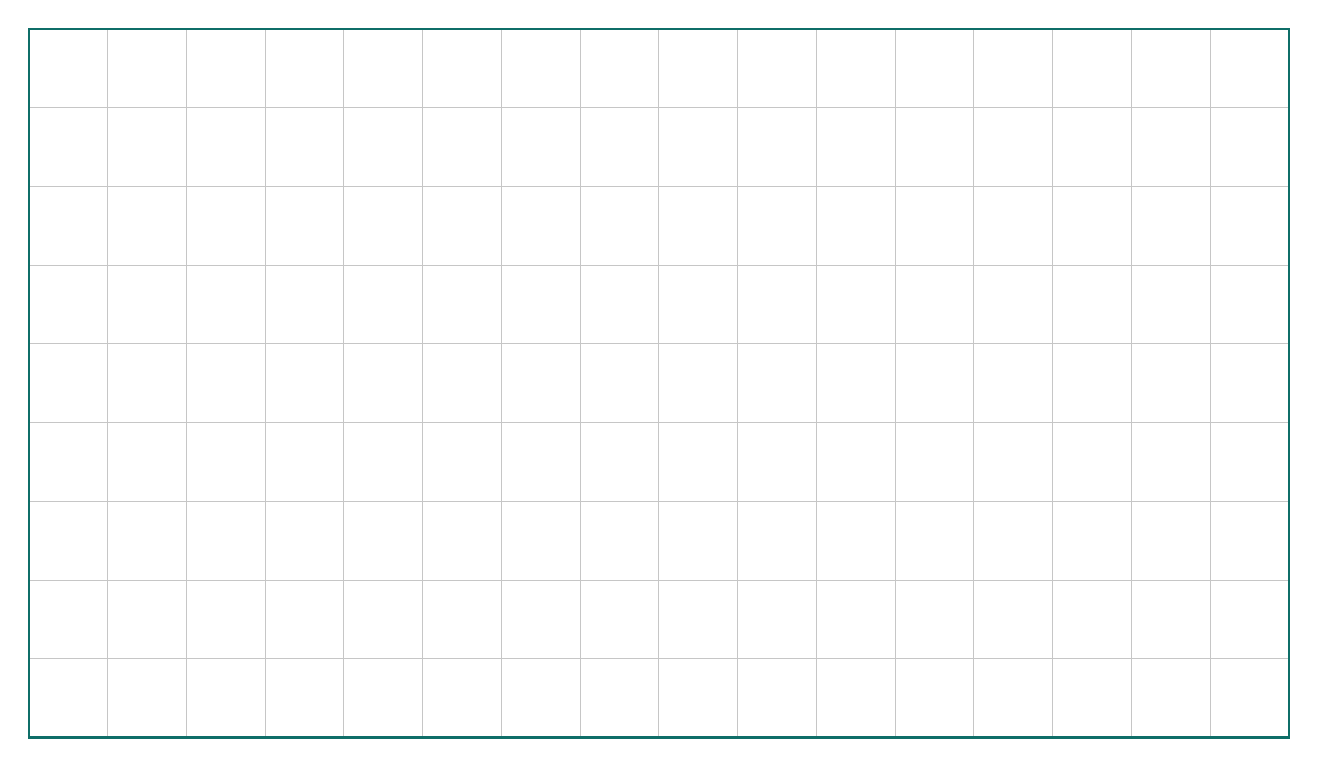
\begin{tikzpicture}
  \draw[step=1cm,gray!45,very thin] (0,0) grid (16,9);
  \draw[mainc,thick] (0,0) rectangle (16,9);
\end{tikzpicture}
\end{center}

\vspace{8pt}
\begin{center}
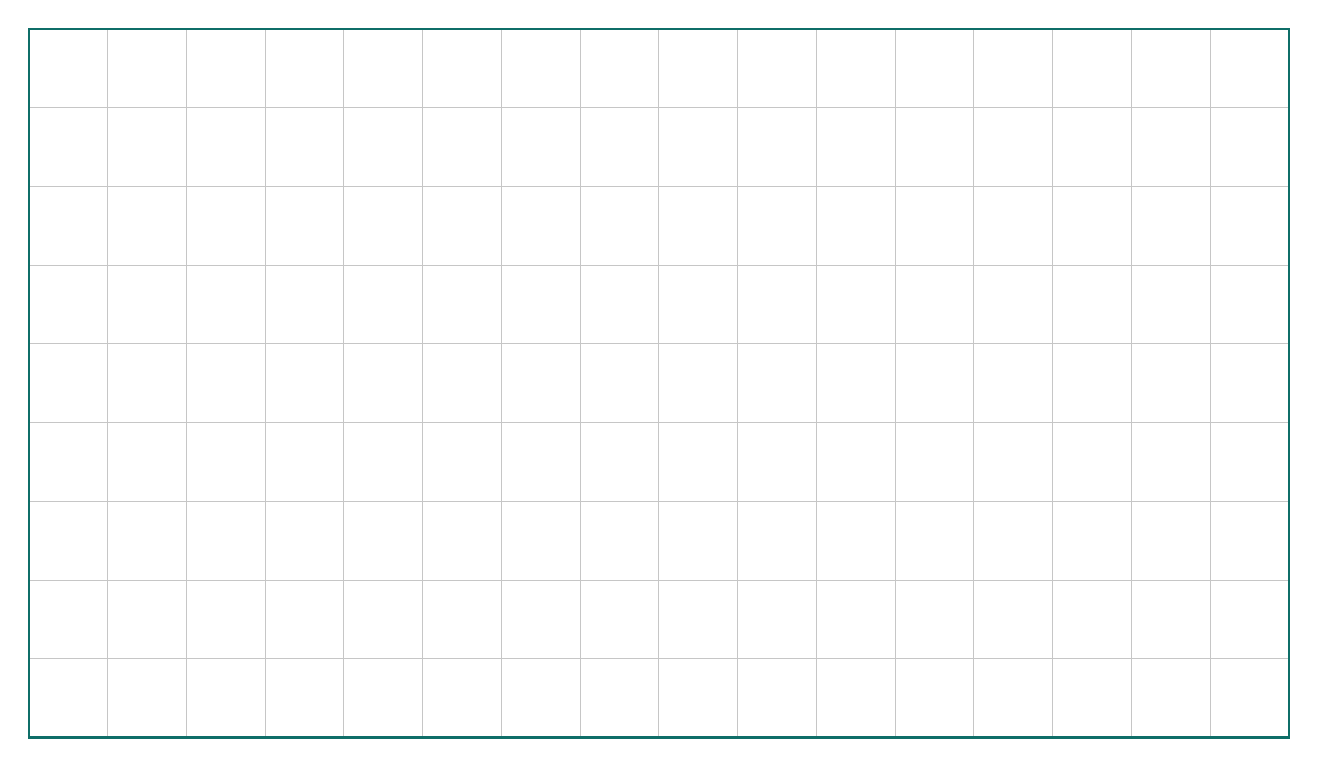
\begin{tikzpicture}
  \draw[step=1cm,gray!45,very thin] (0,0) grid (16,9);
  \draw[mainc,thick] (0,0) rectangle (16,9);
\end{tikzpicture}
\end{center}

\begin{tipbox}
\textbf{怎么用}：\\
① 画线段：起点落在格点上，长度就等于格数（画 5 厘米就数 5 格）；\\
② 点子图：在每个格点上画一个点，就是“几行几列”的点子图；\\
③ 长方形面积（预习）：圈出一个长方形，数里面的格子数，
就是“每行几个 $\times$ 几行”。
\end{tipbox}

\clearpage
\subsection*{B6\quad 竖式练习格（第一单元专用）}

\noindent 每格一个数位，写竖式不会错位。建议印 3 份。

\vspace{6pt}
\begin{center}
\newcommand{\vsframe}{%
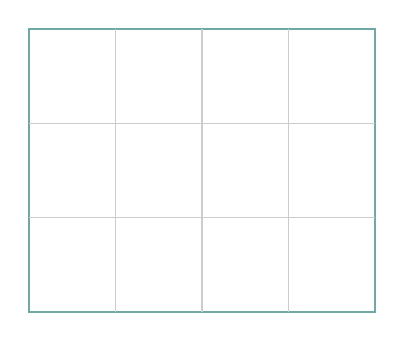
\begin{tikzpicture}
  \draw[mainc!60,thick] (0,0) rectangle (4.4,3.6);
  \draw[gray!40] (0,1.2) -- (4.4,1.2);
  \draw[gray!40] (0,2.4) -- (4.4,2.4);
  \draw[gray!40] (1.1,0) -- (1.1,3.6);
  \draw[gray!40] (2.2,0) -- (2.2,3.6);
  \draw[gray!40] (3.3,0) -- (3.3,3.6);
\end{tikzpicture}}
\vsframe\hspace{0.6cm}\vsframe\hspace{0.6cm}\vsframe

\vspace{0.6cm}
\vsframe\hspace{0.6cm}\vsframe\hspace{0.6cm}\vsframe

\vspace{0.6cm}
\vsframe\hspace{0.6cm}\vsframe\hspace{0.6cm}\vsframe

\vspace{0.6cm}
\vsframe\hspace{0.6cm}\vsframe\hspace{0.6cm}\vsframe
\end{center}

\begin{tipbox}
\textbf{怎么用}：最右一列写个位，中间写十位，最左写百位。
\textbf{进位的小 1 写在十位格子的上边}，\textbf{退位的小点画在十位数字的头顶}。
12 个格子，够做 12 道竖式。
\end{tipbox}

% =============================================================
%  附录 C  模拟人民币（可剪）
% =============================================================
\Chapter{附录 C\quad 模拟人民币（剪开即用）}

\begin{unitinfo}
\textbf{打印}：A4，\textbf{160\,g 卡纸}，单面，100\% 比例（\textbf{不要缩放}）。\\
\textbf{说明}：这是\textbf{课堂教具用}的仿真币，仅为数学学习使用，
不能用于任何真实交易。\\
\textbf{建议印量}：10 元 $\times$2、5 元 $\times$4、1 元 $\times$6、5 角 $\times$8、1 角 $\times$8。
如果家里能直接拿到真币，\textbf{优先用真币}，小豆角的钱感更真实。
\end{unitinfo}

\newcommand{\bill}[3]{%
  \begin{tikzpicture}
    \draw[#3,thick,rounded corners=1.2mm,fill=#3!6] (0,0) rectangle (8.0,4.1);
    \draw[#3!45,thin,rounded corners=1.2mm] (0.28,0.28) rectangle (7.72,3.82);
    \node[font=\scriptsize,color=#3] at (1.7,3.35) {中国人民银行};
    \node[font=\scriptsize,color=#3!70] at (6.2,3.35) {教具用};
    \node[font=\Huge\bfseries,color=#3] at (4.0,1.95) {#1};
    \node[font=\scriptsize,color=#3!75,anchor=south east] at (7.6,0.35) {#2};
  \end{tikzpicture}}

\newcommand{\coin}[2]{%
  \begin{tikzpicture}
    \draw[#2,thick,fill=#2!8] (0,0) circle (1.75);
    \draw[#2!45,thin] (0,0) circle (1.5);
    \node[font=\large\bfseries,color=#2] at (0,0) {#1};
  \end{tikzpicture}}

\subsection*{10 元（印 2 张）}

\begin{center}
\bill{10 元}{拾圆}{sayc}\hspace{0.5cm}\bill{10 元}{拾圆}{sayc}
\end{center}

\subsection*{5 元（印 4 张）}

\begin{center}
\bill{5 元}{伍圆}{playc}\hspace{0.5cm}\bill{5 元}{伍圆}{playc}

\vspace{0.35cm}
\bill{5 元}{伍圆}{playc}\hspace{0.5cm}\bill{5 元}{伍圆}{playc}
\end{center}

\clearpage
\subsection*{1 元（印 6 张）}

\begin{center}
\bill{1 元}{壹圆}{passc}\hspace{0.5cm}\bill{1 元}{壹圆}{passc}

\vspace{0.35cm}
\bill{1 元}{壹圆}{passc}\hspace{0.5cm}\bill{1 元}{壹圆}{passc}

\vspace{0.35cm}
\bill{1 元}{壹圆}{passc}\hspace{0.5cm}\bill{1 元}{壹圆}{passc}
\end{center}

\clearpage
\subsection*{5 角（印 8 个）}

\begin{center}
\coin{5 角}{pitc}\hspace{0.5cm}\coin{5 角}{pitc}\hspace{0.5cm}%
\coin{5 角}{pitc}\hspace{0.5cm}\coin{5 角}{pitc}

\vspace{0.7cm}
\coin{5 角}{pitc}\hspace{0.5cm}\coin{5 角}{pitc}\hspace{0.5cm}%
\coin{5 角}{pitc}\hspace{0.5cm}\coin{5 角}{pitc}
\end{center}

\subsection*{1 角（印 8 个）}

\begin{center}
\coin{1 角}{matc}\hspace{0.5cm}\coin{1 角}{matc}\hspace{0.5cm}%
\coin{1 角}{matc}\hspace{0.5cm}\coin{1 角}{matc}

\vspace{0.7cm}
\coin{1 角}{matc}\hspace{0.5cm}\coin{1 角}{matc}\hspace{0.5cm}%
\coin{1 角}{matc}\hspace{0.5cm}\coin{1 角}{matc}
\end{center}

\clearpage
\subsection*{换算速查（贴墙上）}

\begin{center}
\begin{tabular}{@{}p{6.2cm}p{6.2cm}@{}}
\toprule
\textbf{元与角} & \textbf{角与分} \\
\midrule
$1\ \text{元} = 10\ \text{角}$ & $1\ \text{角} = 10\ \text{分}$ \\
$2\ \text{元} = 20\ \text{角}$ & $5\ \text{角} = 50\ \text{分}$ \\
$5\ \text{元} = 50\ \text{角}$ & $3\ \text{角} = 30\ \text{分}$ \\
$10\ \text{元} = 100\ \text{角}$ & $1\ \text{元} = 100\ \text{分}$ \\
\midrule
\multicolumn{2}{@{}l}{\textbf{换成“几元几角”要练的 6 个}} \\
\midrule
\multicolumn{2}{@{}l}{%
25 角 $=2$ 元 5 角\qquad 38 角 $=3$ 元 8 角\qquad 70 角 $=7$ 元} \\
\multicolumn{2}{@{}l}{%
105 角 $=10$ 元 5 角\qquad 2 元 5 角 $=25$ 角\qquad 7 元 3 角 $=73$ 角} \\
\bottomrule
\end{tabular}
\end{center}

\begin{tipbox}
\textbf{给小豆角的一个小技巧}：\\
看到“几元几角”换算成“角”，就把元数\textbf{后面添一个 0} 再加角数：
2 元 5 角 → 20 + 5 = 25 角；7 元 3 角 → 70 + 3 = 73 角。\\
反过来，看到“几十几角”，就\textbf{把最后一位当角}：38 角 → 3 元 8 角。
\textbf{不要让小豆角背，要让小豆角用“1 元 = 10 角”推一次。}
\end{tipbox}

% =============================================================
%  附录 D  记录表
% =============================================================
\Chapter{附录 D\quad 记录表和速查卡}

\subsection*{D1\quad 走完全册打钩表}

\noindent 上完一次就打个钩，再画颗星。\textbf{41 次全打满，这一册就过完了。}

\begin{center}
\small
\renewcommand{\arraystretch}{1.45}
\begin{tabular}{@{}p{4.4cm}|*{7}{>{\centering\arraybackslash}p{1.15cm}|}@{}}
\hline
\textbf{哪一章} & \textbf{1} & \textbf{2} & \textbf{3} & \textbf{4} & \textbf{5} &
\textbf{6} & \textbf{7} \\
\hline
第一单元\ 加与减（二） & & & & & & & \\ \hline
第二单元\ 测量（一） & & & & & & & \\ \hline
第三单元\ 数一数与乘法 & & & & & & & \\ \hline
第四单元\ 乘法口诀（一） & & & & & & & \\ \hline
第五单元\ 分一分与除法 & & & & & & & \\ \hline
第六单元\ 图形的运动（一） & & & & & & & \\ \hline
第七单元\ 乘法口诀（二） & & & & & & & \\ \hline
第八单元\ 乘除法的应用（一） & & & & & & & \\ \hline
两次综合实践 & & & & & & & \\ \hline
期末复习 & & & & & & & \\ \hline
\end{tabular}
\end{center}

\vspace{4pt}
\noindent{\small 第六单元只有 3 课，第八单元 4 课，综合实践 2 课，
其余 5--6 课。空格多的地方不用硬填满。}

\subsection*{D2\quad 错题本：一次只写一句话}

\noindent\textbf{规矩就一条：只写错在哪，不抄整道题。}
同一个错因出现三次，就停下来回去补那一课。

\begin{center}
\small
\renewcommand{\arraystretch}{1.9}
\begin{tabular}{@{}p{1.7cm}|p{6.6cm}|p{1.9cm}|p{1.4cm}@{}}
\hline
\textbf{日期} & \textbf{错在哪一步（一句话）} & \textbf{重做日期} & \textbf{会了吗} \\
\hline
 & & & \\ \hline
 & & & \\ \hline
 & & & \\ \hline
 & & & \\ \hline
 & & & \\ \hline
 & & & \\ \hline
 & & & \\ \hline
 & & & \\ \hline
 & & & \\ \hline
 & & & \\ \hline
 & & & \\ \hline
 & & & \\ \hline
\end{tabular}
\end{center}

\vspace{2pt}
\noindent\textbf{好的写成长这样}：
\begin{itemize}
  \item “48+25，个位 8+5=13，把进的 1 忘了加到十位”
  \item “52-37，十位 5 借走了 1，还是按 5 减的”
  \item “把‘是 3 倍’当成了‘多 3 个’”
\end{itemize}
\noindent\textbf{没用的写成长这样}：“粗心”“算错了”“不认真”——一条都别写，
写了等于没写。

\clearpage
\subsection*{D3\quad 星星表（攒够 20 颗换奖励）}

\begin{center}
\renewcommand{\arraystretch}{2.5}
\begin{tabular}{|*{5}{>{\centering\arraybackslash}p{2.7cm}|}}
\hline
 & & & & \\ \hline
 & & & & \\ \hline
 & & & & \\ \hline
 & & & & \\ \hline
\end{tabular}
\end{center}

\vspace{6pt}
\begin{center}
\begin{tabular}{@{}p{9cm}p{6cm}@{}}
\toprule
\textbf{怎么得} & \textbf{几颗} \\
\midrule
一次课顺顺当当上完（不哭、不跑、不超时） & \starx \\
一次“5 分钟快检”全对 & \starx \\
\textbf{小豆角自己发现并改了一个错} & \starx\starx \\
一周每天都做了 3 分钟口算卡 & \starx \\
\bottomrule
\end{tabular}
\end{center}

\clearpage
\subsection*{D4\quad 剪下来贴冰箱的那张}

\begin{center}
\begin{tcolorbox}[enhanced,colback=white,colframe=mainc,boxrule=1.2pt,
                  arc=2mm,width=16.6cm,left=10pt,right=10pt,top=8pt,bottom=8pt]
\begin{center}
{\heiti\large 每次二十分钟，就这么切}\\[4pt]
\renewcommand{\arraystretch}{1.35}
\begin{tabular}{@{}p{2.2cm}p{2.6cm}p{9.6cm}@{}}
\toprule
3 分钟 & 抽卡口算 & 抽 10 张，只记对错，当场不纠 \\
2 分钟 & 小豆角自己读题 & 只说一句“把数字圈出来”，豆角爸爸不念题 \\
8 分钟 & \textbf{上手摆} & \textbf{全场最重要，豆角爸爸不可以说话} \\
5 分钟 & 落到纸上 & 写算式／竖式／口诀，豆角爸爸不代笔 \\
2 分钟 & 收尾 & 三问：学了啥／哪步易错／还来一次吗 \\
\bottomrule
\end{tabular}
\end{center}
\end{tcolorbox}
\end{center}

\begin{center}
\begin{tcolorbox}[enhanced,colback=white,colframe=pitc,boxrule=1.2pt,
                  arc=2mm,width=16.6cm,left=10pt,right=10pt,top=8pt,bottom=8pt]
\begin{center}
{\heiti\large 六件豆角爸爸最不该做的事}\\[4pt]
\begin{tabular}{@{}p{0.6cm}p{14.2cm}@{}}
1 & 把规则直接说出口（让小豆角自己摆出来） \\
2 & 拿口诀顶替理解（每句新口诀先圈图） \\
3 & 管小豆角掰手指（二年级上学期正常，别管） \\
4 & 用题量顶思考（一种类型做透 5 道） \\
5 & 边做边纠错（整道题做完再回头看） \\
6 & 盯着分数（能说清“为什么”才是目标） \\
\end{tabular}
\end{center}
\end{tcolorbox}
\end{center}

\begin{center}
\begin{tcolorbox}[enhanced,colback=white,colframe=passc,boxrule=1.2pt,
                  arc=2mm,width=16.6cm,left=10pt,right=10pt,top=8pt,bottom=8pt]
\begin{center}
{\heiti\large 小豆角卡住了，就问这三句}\\[4pt]
{\kaishu ① “小豆角是怎么想的？”\quad ② “这一捆／这一份是从哪来的？”\quad
③ “小豆角能画出来给爸爸看吗？”}\\[3pt]
{\small 三句都不管用 $\to$ 换材料（小棒换豆子、纸换白板）$\to$ 还不行就今天先停，
明天再来。\textbf{停下来永远比硬推有用。}}
\end{center}
\end{tcolorbox}
\end{center}

% =============================================================
%  附录 E  过关奖状
% =============================================================
\Chapter{附录 E\quad 过关奖状}

\begin{unitinfo}
两张证，一张是打完第一关发的，一张是全打完发的。
\textbf{打印在好一点的纸上，签上字，颁发给小豆角}\\
\end{unitinfo}

\begin{center}
\begin{tcolorbox}[enhanced,colback=white,colframe=matc,boxrule=2pt,arc=3mm,
                  width=15.6cm,left=12pt,right=12pt,top=12pt,bottom=12pt]
\begin{center}
{\heiti\Large\color{matc} 第一关通关证书}\\[8pt]
{\kaishu\large
兹证明\ {\Large\underline{\hspace{5cm}}}\ 同学，\\[6pt]
独立完成了“一串小棒走天下”全部任务，\\[4pt]
\textbf{能自己把十根小棒捆成一捆，并说清“这一捆从哪来”}。\\[10pt]
星级评价：\ \starx\ \starx\ \starx\ \starx\ \starx\\[10pt]
\begin{tabular}{@{}p{6cm}p{6cm}@{}}
家长签字：\underline{\hspace{3.2cm}} & 日期：\underline{\hspace{3.2cm}}\\
\end{tabular}}
\end{center}
\end{tcolorbox}
\end{center}

\vspace{6pt}
\begin{center}
\begin{tcolorbox}[enhanced,colback=white,colframe=mainc,boxrule=2pt,arc=3mm,
                  width=15.6cm,left=12pt,right=12pt,top=12pt,bottom=12pt]
\begin{center}
{\heiti\Large\color{mainc} 全册通关证书}\\[8pt]
{\kaishu\large
兹证明\ {\Large\underline{\hspace{5cm}}}\ 同学，\\[6pt]
打完八个关卡，加一个隐藏关，\\[4pt]
\textbf{能自己讲明白“为什么满十要进一”“为什么除法想口诀”“为什么拆开就好算”}。\\[10pt]
累计星星：\underline{\hspace{2.4cm}}\ 颗\\[8pt]
最难忘的一次翻车：\underline{\hspace{8cm}}\\[10pt]
\begin{tabular}{@{}p{6cm}p{6cm}@{}}
家长签字：\underline{\hspace{3.2cm}} & 日期：\underline{\hspace{3.2cm}}\\
\end{tabular}}
\end{center}
\end{tcolorbox}
\end{center}

% =============================================================
%  附录 F  课前协商记录
% =============================================================
\Chapter{附录 F\quad 课前协商记录}

\begin{unitinfo}
每关上课前，在这里写下今天谈定的赌注，双方签字；打完一关划一行。
\end{unitinfo}

\begin{center}
\small
\renewcommand{\arraystretch}{1.85}
\begin{tabularx}{\linewidth}{@{}p{0.8cm}p{2.0cm}Xp{2.2cm}p{1.5cm}@{}}
\hline
\textbf{关} & \textbf{日期} & \textbf{今天谈定的赌注（手写）} & \textbf{谁赢} & \textbf{兑现} \\
\hline
1 & & & & \\ \hline
2 & & & & \\ \hline
3 & & & & \\ \hline
4 & & & & \\ \hline
5 & & & & \\ \hline
6 & & & & \\ \hline
7 & & & & \\ \hline
8 & & & & \\ \hline
9 & & & & \\ \hline
10 & & & & \\ \hline
\end{tabularx}
\end{center}

\vspace{0.3cm}

\begin{tipbox}
\textbf{谈的时候记住三条}：\\
① \textbf{先让小豆角开口提}。她自己提的赌注，她才认账。\\
② \textbf{当场兑现}。拖到第二天，这个赌就不灵了。\\
③ \textbf{这张表只记输赢和兑现}，不用来评价谁学得好——它不是第二个考卷。
\end{tipbox}

\vspace{0.2cm}



% ---------- 后记（内容最后一页，单独一页） ----------
% =============================================================
%  后记
% =============================================================
\ctexset{section/numbering=false}

\Chapter{后记}

\vspace{0.4cm}

写完这份执行手册，感觉有点人格分裂。

写的过程先要摆脱“豆角爸爸”这个当事人的身份，把自己变成小豆角学校的老师，同时又是小豆角本人——
先以“老师”的身份教会“学生”，以“学生”的身份判断老师讲的是否足够简单易懂，以此判断自己讲的东西
是否被自己理解，形成逻辑闭环，然后从“学生”切换成“豆角爸爸”，再以“豆角爸爸”的身份来模拟跟小豆
角互动，以此来指导遣词造句细节。

一会儿站在岸上，一会儿泡在水里，逻辑难免混乱。

不过整书复核、校对下来，勉强能用了。先用着吧。

\vfill

\begin{center}
{\kaishu\large 豆角爸爸}\\[4pt]
{\small\color{tipc} https://www.bd7iwd.com}
\end{center}

\vspace{0.6cm}


% ---------- 补白页（自动补到偶数页，胶装用；无页眉页码） ----------
\clearpage
\makeatletter
\ifodd\c@page\else
  \null\thispagestyle{empty}\clearpage
\fi
\makeatother

\end{document}
